%#!platex main
\documentclass[a4j,10pt]{jsbook}
\usepackage[dvipdfmx]{graphicx}
\usepackage{listings}
\usepackage{latexsym}
\usepackage{ascmac}
\usepackage{amsmath}
\usepackage{amssymb}
%\usepackage{mediabb}

\title{「コンパイラ」講義ノート}
\author{国島丈生}

\newtheorem{theorem}{定理}[chapter]
\newtheorem{example}{例}[chapter]
\newtheorem{definition}{定義}[chapter]
\newtheorem{exercise}{問題}[chapter]

\newcommand{\icode}[1]{{\sf #1}}

\lstset{language=C,basicstyle=\footnotesize\ttfamily}
\lstloadlanguages{[x86masm]Assembler}

\DeclareMathOperator{\op}{op}

\begin{document}
\maketitle

%#!platex main

\chapter{$BF3F~(B}
\label{134138_29Mar06}

$BK\9V5A$G$O!"%3%s%Q%$%i$NFbIt9=@.$K$D$$$F!"M}O@LL$+$i<B:]$N%W%m%0%i%`$K;j(B
$B$k$^$G$r07$&!#(B

C$B8@8l$N%3%s%Q%$%i$O1i=,!&<B83Ey$G$h$/;H$C$F$$$k$O$:$G$"$k!#$3$N%=%U%H%&%'(B
$B%"$O!"(BC$B8@8l$N%W%m%0%i%`$r5!3#8l$N%W%m%0%i%`$d<B9T7A<0%U%!%$%k(B
$B!J(B\icode{a.out}$B$J$I!K$KJQ49$7$F$/$l$k!#0lHL$K(B{\bfseries $B%3%s%Q%$(B
$B%i(B}$B!J(Bcompiler$B!K$H$O!"!V$"$k%W%m%0%i%_%s%08@8l$G=q$+$l$?%W%m%0%i%`$rFI$_9~(B
$B$s$G!"JL$N%W%m%0%i%_%s%08@8l$K$h$kEy2A$J%W%m%0%i%`$KK]Lu$9$k%=%U%H%&%'%"!W(B
$B$G$"$k!#K]LuA0$N%W%m%0%i%_%s%08@8l$r(B{\bfseries $B86;O8@8l(B}$B!J(Bsource
language$B!K!"K]Lu8e$N%W%m%0%i%_%s%08@8l$r(B{\bfseries $BL\E*8@8l(B}$B!J(Btarget
language$B!K$H$$$&!#$^$?!"K]LuA0$N%W%m%0%i%`$r(B{\bfseries $B86;O%W%m%0%i(B
$B%`(B}$B!J(Bsource program$B!K!"K]Lu8e$N%W%m%0%i%`$r(B{\bfseries $BL\E*%W%m%0%i(B
$B%`(B}$B!J(Btarget program$B!K$H$$$&!#(BC$B8@8l$N%3%s%Q%$%i$O!"86;O8@8l$,(BC$B!"L\E*8@8l$,(B
$B5!3#8l$G$"$k$h$&$J%3%s%Q%$%i(B\footnote{\icode{gcc}$B$O!"(BC$B0J30$N8@8l!J(BC++$B$J$I!K(B
$B$b86;O8@8l$H$7$F07$($k!#(B}$B$G$"$k!#$^$?%3%s%Q%$%i$O!"86;O%W%m%0%i%`$r2r@O$7!"(B
$B$=$NCf$KJ8K!E*$J8m$j$,$"$l$P!"$=$N$3$H$r%f!<%6$KDLCN$7$F$/$l$k!#(B

$B%3%s%Q%$%i$NNr;K$O(B1950$BG/Be$K$5$+$N$\$k!#Ev;~$O!"%3%s%Q%$%i$O<BAu$K$R$I$/(B
$B<j4V$N$+$+$k%=%U%H%&%'%"$G$"$C$?!#$7$+$7!"$=$N8e(B1980$BG/Be:"$^$G$K!"%3%s%Q(B
$B%$%i@_7W$K4X$9$kM}O@E*$+$DBN7OE*$J<jK!$,$$$m$$$m9M0F$5$l!"%3%s%Q%$%i<BAu(B
$B$NB?$/$NItJ,$O<+F0$G9T$($k$h$&$K$J$C$?!#(B

$B$7$?$,$C$F%3%s%Q%$%i$N@_7W5;K!$O!">pJs2J3X!"%O!<%I%&%'%"!"%=%U%H%&%'%"$N(B
3$BJ,Ln$,8r:9$9$k$H$3$m$K$"$j!"4XO"2JL\$bB?4t$KEO$k!#(B
\begin{description}
 \item[$B@h9T2JL\(B] $B>pJs=hM}3X!"N%;6?t3X!"%W%m%0%i%_%s%08@8l(BI$B!"%W%m%0%i%_%s%08@8l(BII$B!"7W;;5!%"!<%-%F%/%A%c(BA
 \item[$B8eB32JL\(B] $B7A<08@8lM}O@!J=$;N!K(B
\end{description}
$B$3$N$[$+!"$3$N9V5A$G$O%W%m%0%i%`Nc$N5-=R$K(BC$B8@8l$rMQ$$$k!#$=$N$?$a!"9V5AA4(B
$BHL$rDL$7$F(BC$B8@8l$NCN<1$,I,MW$K$J$k!#(B

$B$3$N9V5A$O(B
\cite{aho86:_compiler}\cite{aho07:_compil_princ_techn_tools_secon_edition}
\cite{$BEr@u(B01}$B$r4p$K$7$F$$$k!#$?$@$7!"J,NL$,KDBg$G$"$j!"$+$DFq2r$JItJ,$bB?(B
$B$$$N$G!"4pACE*$JItJ,$rH4?h$7$F9=@.$7$F$$$k(B\footnote{$BK\%F%-%9%HCf$NNc$K$D(B
$B$$$F$O$3$l$i$N=q@R$+$i$N0zMQ$,$+$J$jB?$/!"3X304X78<T$KN.I[$9$k$HCx:n8">e(B
$BLdBj$,$"$k!#K\;qNA$NMxMQ$O3XFb4X78<T$N$_$K$H$I$a$F$*$$$F$$$?$@$-$?$$!#(B}$B!#$=$NB>!"(B
\cite{$B%[%C%W%/%m%U%H(B03:automaton}\cite{$BCfED(B99}\cite{$B%+!<%K%O%s(B89}$B$J$I$rE,(B
$B59;2>H$7$F$$$k!#(B

\section{$B%3%s%Q%$%i$N9=@.(B}
\label{134201_29Mar06}

$B:#8e$N9V5A$NN.$l$rCN$C$F$*$/$?$a$K!"Nc$rMQ$$$F%3%s%Q%$%i$NFbIt9=@.$r4JC1(B
$B$K@bL@$9$k$3$H$K$7$h$&!#<!$N(BC$B%W%m%0%i%`!J(B\icode{simple.c}$B!K$r9M$($k!#(B

\begin{quote}
\lstinputlisting{code/simple.c}
\end{quote}

\begin{figure}
 \lstinputlisting[language={[x86masm]Assembler},numbers=left,xleftmargin=100pt]{code/simple.s}
 \caption{i386$B5!3#8lL?Na$NNc(B}
 \label{143232_11Apr06}
\end{figure}

$B%3%s%Q%$%i$O(B\icode{simple.c}$B$NFbMF$r2r@O$7!"Nc$($P?^(B\ref{143232_11Apr06}
$B$N$h$&$J5!3#8lNs$r@8@.$9$k(B\footnote{i386$B%"!<%-%F%/%A%c$r2>Dj$7$F$$$k!#(B}$B!#(B
$B$J$*!"K\Ev$N5!3#8lNs$O!"$=$l$>$l$N%7%s%\%k$r(B0/1$B$NNs$GCV$-49$($?$b$N$K$J$k!#(B

$B3F5!3#8lL?Na$O!"(BCPU$B$K$h$C$FD>@\2r<a<B9T$9$k$3$H$,$G$-$k!#(B
\icode{simple.c}$B$r%3%s%Q%$%k$7$FF@$i$l$?<B9T7A<0%U%!%$%k!J(B\icode{a.out}$B$J(B
$B$I!K$r<B9T$9$k$H!"$3$N5!3#8lL?NaNs$,<g5-21>e$K%m!<%I$5$l!"(BCPU$B$,$=$l$r=g<!(B
$B2r<a$7$F<B9T$7$F$$$/!#3F9T$N0UL#$O$@$$$?$$<!$N$h$&$K$J$C$F$$$k!#(B
\begin{itemize}
 \item 3$B9TL\!D(B\icode{\_main}$B$H$$$&L\0u!J%i%Y%k!K$E$1!#(B\icode{main}$B4X?t$KBP(B
       $B1~$7$F$$$k!#(B
 \item 4-6$B9TL\!D(B\icode{main}$B4X?t$N8F$S=P$7=hM}!#$3$N$H$-!"(B
       \icode{-16(\%ebp)}$BHVCO$+$i(B4$B%P%$%H$NNN0h$K6I=jJQ?t(B\icode{x}$B$,!"(B
       \icode{-12(\%ebp)}$BHVCO$+$i(B4$B%P%$%H$NNN0h$K6I=jJQ?t(B\icode{y}$B$,$=$l$>(B
       $B$l3d$jEv$F$i$l$k!#(B
 \item 7$B9TL\!D(B\icode{y}$B$NNN0h$K(B\icode{\$1}$B!"$9$J$o$ADj?t(B1$B$,%;%C%H$5$l$k!#(B
 \item 8$B9TL\!D(B\icode{y}$B$NNN0h$NCM$,%l%8%9%?(B\icode{\%eax}$B$K%;%C%H$5$l$k!#(B
 \item 9$B9TL\!D%l%8%9%?(B\icode{\%eax}$B$NCM$KDj?t(B20$B$,2C$($i$l$k!#(B
 \item 10$B9TL\!D%l%8%9%?(B\icode{\%eax}$B$NCM$,(B\icode{x}$B$NNN0h$K%;%C%H$5$l$k!#(B
 \item 11-13$B9TL\!D(B\icode{main}$B4X?t$N=*N;=hM}(B\footnote{11-12$B9TL\$O(B
       \icode{leave}$B$H$$$&(B1$B$D$N5!3#8lL?Na$K$^$H$a$i$l$F$$$k$3$H$b$"$k!#(B}$B!#(B
\end{itemize}

$B$3$N9V5A$G07$&FbMF$r@0M}$9$k$H<!$N$h$&$K$J$k!#(B
\begin{enumerate}
 \item $B86;O%W%m%0%i%`!J>e$NNc$G$O(BC$B%W%m%0%i%`!K$+$iL\E*%W%m%0%i%`!J>e$NNc(B
       $B$G$O5!3#8lNs!K$r@8@.$9$k%"%k%4%j%:%`(B\label{195753_28Mar06}
 \item \ref{195753_28Mar06}$B$r<B8=$9$k%W%m%0%i%`(B
       \label{195816_28Mar06}
 \item \ref{195816_28Mar06}$B$r<+F0E*$K@8@.$9$k%"%k%4%j%:%`(B/$B<jK!(B
       \label{200119_28Mar06}
\end{enumerate}
\ref{195753_28Mar06}$B$H(B\ref{200119_28Mar06}$B$N0c$$$K=<J,N10U$5$l$?$$!#(B

$B$5$F!"%3%s%Q%$%i$OBg$-$/J,$1$F0J2<$N(B2$B$D$NItJ,$+$i9=@.$5$l$k!#(B
\begin{description}
 \item[$B2r@OIt(B] $B86;O%W%m%0%i%`$r2r@O$7!"%3%s%Q%$%iFbIt$G=hM}$9$k$?$a$N%G!<(B
	    $B%?9=B$!J(B{\bfseries $BCf4VI=8=(B}$B!K$r:n$k!#J8;zNs$H$7$F$N86;O%W%m(B
	    $B%0%i%`$+$i%W%m%0%i%`$N:G>.0UL#C10L!J(B{\bfseries $B%H!<%/%s(B},
	    token$B!K$r@Z$j=P$9(B{\bfseries $B;z6g2r@O(B}$B!J(Blexical analysis$B!KIt!"(B
	    $B%H!<%/%sNs$+$i%W%m%0%i%`$N0UL#9=B$$r2r@O$9$k(B{\bfseries $B9=J82r(B
	    $B@O(B}$B!J(Bsyntax analysis$B!KIt!"7?$N8!::$J$I9=J82r@OIt$G$O9T(B
	    $B$($J$$%W%m%0%i%`2r@O$r9T$&(B{\bfseries $B0UL#2r@O(B}$B!J(Bsemantic
	    analysis$B!KIt$N(B3$B$D$NItJ,$+$i$J$k!#$^$?!"@h$NNc$N(B\icode{main},
	    \icode{x}, \icode{y}$B$J$I!"%f!<%6$,Dj5A$7$?JQ?t$d4X?t$NNs5s$b(B
	    $B$3$NCJ3,$G9T$o$l$k!#(B
 \item[$B9g@.It(B] $B2r@OIt$G:n$C$?Cf4VI=8=$r4p$K!"L\E*%W%m%0%i%`$r9g@.$9$k!#>l(B
	    $B9g$K$h$C$F$O!"<B9TB.EY$r>e$2$k$?$a$K!"9g@.$7$?%W%m%0%i%`$r$5(B
	    $B$i$K2C9)$9$k$3$H$b$"$k!J(B{\bfseries $B:GE,2=(B}, optimization$B!K!#(B
\end{description}

$B%3%s%Q%$%i$O!":G=i$O86;O%W%m%0%i%`$rC1$J$kJ8;z$NJB$S$H$7$F07$&!#@h$NNc$G(B
$B8@$($P!"<!$N$h$&$JJ8;z$NJB$S$H$7$F07$&!J(B\verb|\n|$B$O2~9TJ8;z$rI=$9!K!#(B
\begin{quote}
\verb|int main()\n{\n int x;\n int y = 1;\n x = y + 20;\n}\n|
\end{quote}
$B$3$3$+$i(BC$B8@8l$H$7$F0UL#$N$"$kJ8;zNs$r@Z$j=P$9$N$,;z6g2r@OIt$G$"$k!#7k2L$O(B
$B<!$N$h$&$JJ8;zNs$NJB$S$K$J$k(B\footnote{$B8e$G=R$Y$k$h$&$K!"<B:]$K$O!"=PNO$9(B
$B$k$N$O$=$l$>$l$NJ8;zNs$rCj>]2=$7$?5-9f!"$9$J$o$A%H!<%/%s$G$"$k!#$^$?!"0l(B
$BEY$K$3$N$h$&$JJB$S$r$^$H$a$F=PNO$9$k$N$G$O$J$/!";z6g2r@OIt$KMW5a$,$"$k$?(B
$B$S$K0l$D$:$D@Z$j=P$7$F=PNO$9$k!#(B}$B!#6uGr$d2~9TJ8;z$J$I!"(BC$B8@8l$H$7$F0UL#$N(B
$B$J$$J8;zNs$O=PNO$5$l$F$$$J$$$3$H$KCm0U$7$F$*$$$F$[$7$$!#(B
\begin{quote}
 \verb|int|, \verb|main|, \verb|(|, \verb|)|, \verb|{|, \verb|int|,
 \verb|x|, \verb|;|, \verb|int|, \verb|y|, \verb|=|, \verb|1|, 
 \verb|;|, \verb|x|, \verb|=|, \verb|y|, \verb|+|, \verb|20|, \verb|;|,
 \verb|}|
\end{quote}

$B$3$NJB$S$r!"%W%m%0%i%_%s%08@8l$NJ8K!$K=>$C$F%0%k!<%W2=$7!"0UL#$N$^$H$^$j(B
$B$r2r@O$9$k$N$,9=J82r@OIt$G$"$k!#Nc$($P!"%;%_%3%m%s(B \verb|;| $B$O(BC$B8@8l$NJ8$N6h(B
$B@Z$j$G$"$j!"%;%_%3%m%s$G0O$^$l$?<!$NItJ,$O0l$D$N$^$H$^$j$K$J$k!#(B
\begin{quote}
 \verb|x|, \verb|=|, \verb|y|, \verb|+|, \verb|20|
\end{quote}
$B$3$l$O$5$i$K(B\verb|x|, \verb|=|, \verb|y| \verb|+| \verb|20|$B$H$$$&(B3$B$D$NIt(B
$BJ,$K%0%k!<%W2=$G$-!"$5$i$K:G8e$NItJ,$O(B\verb|y|, \verb|+|, \verb|20|$B$H$$$&(B
3$B$D$NItJ,$K%0%k!<%W2=$G$-$k!#$3$N$h$&$K!"%0%k!<%W2=$7$?7k2L!"$D$^$j9=J82r(B
$B@O$N7k2L$ODL>o%0%k!<%W$NF~$l;R$K$J$j!"LZ$GI=8=$9$k$N$,0lHLE*$G$"$k!J?^(B
\ref{112135_29Mar06}$B!K!#O@M}E*$K$O!"$3$l$,9=J82r@OIt$N=PNO%G!<%?9=B$$K$J(B
$B$k!#(B

\begin{figure}
 \begin{center}
  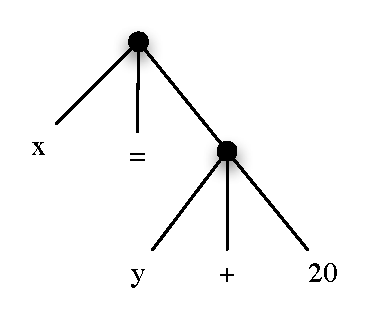
\includegraphics[scale=0.8]{figure/tree_structure.pdf}
 \end{center}
 \caption{{\sffamily x = y + 20}$B$rI=$9LZ9=B$(B}
 \label{112135_29Mar06}
\end{figure}

$B$3$NLZ$K$O!"7?$N>pJs$J$I!"%W%m%0%i%`<B9T$N$?$a$N=EMW$J>pJs$,$$$/$D$+4^$^(B
$B$l$F$$$J$$!#$3$l$rJd$&$N$,0UL#2r@OIt$G$"$k!#Dj?t$dJQ?t$N7?JQ49$J$I$O0UL#(B
$B2r@OIt$GE,59=hM}$5$l$k!#$=$N7k2L!"9=J82r@OIt$N=PNO$NLZ$K=$@5$,2C$($i$l$k(B
$B$3$H$b$"$k!#(B

$B$3$3$^$G$GF@$i$l$?LZ9=B$$r4p$K$7$F!"L\E*%W%m%0%i%`$,9g@.$5$l$k!#$=$N:]!"(B
$B$$$-$J$jL\E*%W%m%0%i%`$r9g@.$9$k$N$G$O$J$/!"$$$C$?$s5<;wE*$J5!3#8lNs$r@8(B
$B@.$7$F$+$i<B:]$NL\E*%W%m%0%i%`$KJQ49$9$k$[$&$,9M$($d$9$$!#Nc$($P!"(B
{\sffamily x = y + 20}$B$KBP$7$F!"?7$?$JJQ?t(B\icode{temp1}, \icode{temp2}$B$r(B
$BF3F~$7!"<!$N$h$&$J5<;w5!3#8lNs$r9M$($k!#(B
\begin{quote}
\begin{verbatim}
	temp1 = y
	temp2 = temp1 + 20
	x = temp2
\end{verbatim}
\end{quote}
$B$9$k$H!"@h$K<($7$?L\E*%W%m%0%i%`$H$NBP1~$,$H$j$d$9$/$J$k$3$H$,J,$+$k$@$m(B
$B$&!#$3$N5<;w5!3#8lNs$KBP$7$F!"JQ?t(B\icode{temp1}, \icode{temp2}$B$K%l%8%9%?(B
\icode{\%eax}$B$r!"(B\icode{x}$B$KHVCO(B\icode{-16(\%ebp)}$B$r!"(B\icode{y}$B$KHVCO(B
\icode{-12(\%ebp)}$B$r$=$l$>$l3d$jEv$F$k$H!"@h$K<($7$?L\E*%W%m%0%i%`$,@8@.(B
$B$G$-$k!#%l%8%9%?$dHVCO$N3d$jEv$F!"4X?t8F$S=P$7;~$N=hM}%3!<%I$NDI2C$J$I$b(B
$B9g@.It$G9T$o$l$k!#(B

$B$J$*!"$3$3$G=R$Y$?%3%s%Q%$%i$N9=@.$O$b$C$H$b4pK\E*$J$b$N$G$"$k!#<B:]$N%3(B
$B%s%Q%$%i@_7W$G$O$3$N9=@.$K87L)$K$O=>$o$J$$$3$H$bB?!9$"$k!#(B

\section{$BN}=,LdBj(B}

\begin{exercise}
\label{ex:intro01}
 \icode{gcc}$B$O!"(B\icode{-s}$B%*%W%7%g%s$r$D$1$k$3$H$G5!3#8lL?NaNs$r=PNO$5$;(B
 $B$k$3$H$,$G$-$k!#4JC1$J(BC$B8@8l%W%m%0%i%`$r3F<+$G=q$-!"$I$N$h$&$J5!3#8lL?Na(B
 $BNs$,=PNO$5$l$k$+!";n$7$F$_$h!#(B
\end{exercise}
\begin{exercise}
\label{ex:intro02}
 $B<!$N(BC$B8@8l$NJ8$r!"(BC$B8@8l$H$7$F0UL#$N$"$kJ8;zNs$KJ,2r$;$h!#(B
 \begin{quote}
  \verb|x = 0; while (i < 100) { x += i; i++; }|
 \end{quote}
\end{exercise}

%#!platex main

\chapter{正則表現と有限オートマトン}
\label{175712_30Mar06}

コンパイラの技法のうち、字句解析と構文解析は言語理論と関連が深い。ここで
は言語理論で用いられる用語を簡単に説明し、次いで字句解析で用いられる正則
表現と有限オートマトンについて述べる。構文解析で用いられる文脈自由文法に
ついては\ref{151253_30Mar06}章で述べる。

\section{アルファベットと記号列}

普段われわれが「文字」と呼んでいるもの
を、言語理論では{\bfseries 記号}(symbol)といい、また、記号の有限集合を
{\bf アルファベット}(alphabet)という\footnote{日常生活で英文字を
表すときに用いる「アルファベット」とは意味が異なる。}。
\begin{example}
 $\{a, b, \cdots, z\}$や$\{0, 1\}$はアルファベットである。$\Box$
\end{example}
記号が「文字」を表さないこともある。例えば、コンパイラの字句解析部では記号を
「文字」と考えてよいが、構文解析部では、記号は原始言語で意味のある文字列、
すなわちトークンである。

アルファベット$\Sigma$\footnote{アルファベットはしばしば$\Sigma$と表され
る。}中の記号からなる有限列を、$\Sigma$上の{\bf 記号列}(string)と
いう\footnote{文字列、あるいは語(word)ということもある。}。$\Sigma$上の
記号列$s$について、$s$に現れる記号の数を$s$の{\bf 長さ}といい、
$|s|$で表す。

\begin{example}
 $main$や$exercise$はアルファベット$\{a, b, \cdots, z\}$上の記号列であり、
 長さはそれぞれ$4, 8$である。また$\epsilon, 0, 11, 01011$はいずれもアルファ
 ベット$\{0, 1\}$上の記号列であり、長さはそれぞれ$0, 1, 2, 5$である。
 $\Box$
\end{example}

長さ0の記号列、つまり1つも記号を含まない記号列を{\bf 空列}(empty string)
といい、$\epsilon$という記法で表す。$|\epsilon| = 0$である。

\section{言語}

言語理論での{\bf 言語}(language)とは、日本語や英語、プログラミン
グ言語などを抽象化したものである。

アルファベット$\Sigma$上の{\bf 言語}(language)とは、$\Sigma$上の
記号列の集合である。言語に含まれる記号列は可算無限でも構わない。

\begin{example}
 $\{0\}$, $\{00, 01, 10, 11\}$, $\{1, 11, 111, 1111, \cdots\}$はいずれも
 アルファベット$\{0, 1\}$上の言語であり、それぞれ記号列$0$、長さ2のすべて
 の記号列、記号$1$のみからなるすべての記号列を表す。$\Box$
\end{example}

言語は記号列の集合であるから、空集合$\emptyset$や、空列しか含まない集合
$\{\epsilon\}$も言語である。この2 つの言語は全く異なるものであることに充
分注意しておいてほしい。$\emptyset$には要素は1つも含まれないが、
$\{\epsilon\}$には$\epsilon$という要素が1つ含まれている。

\section{言語に対する演算}

言語は(記号列の)集合であるので、$\cup,\; \cap,\; \bar{\;}$(補集合)などの
集合演算はもちろん適用できる。その他に、記号列に由来する重要な演算がいく
つかある。

\subsection{連接}

まず、{\bf 連接}という演算を紹介しよう。そのために、記号列に対する連接を定義し
ておく。2つの記号列$x, y$について、$x$の後ろに$y$が続く記号列を$x$
と$y$の{\bf 連接}(concatenation)といい、$x\cdot y$または$xy$と書
く。
\begin{example}
 $00\cdot 11 = 0011$, $111\cdot \epsilon = \epsilon\cdot 111 = 111$であ
 る。$\Box$
\end{example}

任意の記号列$x$に対して$\epsilon\cdot x = x\cdot\epsilon = x$が成り立つ。
つまり、$\epsilon$は連接に関する単位元である。

記号列$x$自身を$n$個連接した記号列を$x^n$と表し、特に
$x^0=\epsilon$と定義しておく。この結果、$i\geq 0,\, j\geq 0$に対して
$x^{i+j} = x^i\cdot x^j$が成立する。

\begin{example}
 $(01)^2 = 0101, (01)^3 = 010101$ である。$\Box$
\end{example}

さて、2つの言語$L, M$に対する連接$\cdot$を次のように定義する。
\begin{equation*}
  L\cdot M = \{s\cdot t \mid s \in L, t \in M\}
\end{equation*}
記号列の連接と同様、$\cdot$を省略して$LM$と書くこともできる。

\begin{example}
 $L = \{0, 1\}, M = \{0, 01, 111\}$とすると、
 $L\cdot M = \{00, 001, 0111, 10, 101, 1111\}$である。また
 $L \cdot \{\epsilon\} = \{\epsilon\}\cdot L = L$, 
 $M\cdot \emptyset = \emptyset \cdot M = \emptyset$である。$\Box$
\end{example}

任意の言語$L$に対し$L\cdot \{\epsilon\} = \{\epsilon\}\cdot L
= L$が成り立つ。また$L\cdot \emptyset = \emptyset\cdot L = \emptyset$が成
り立つ。つまり、言語の連接では、$\{\epsilon\}$が単位元、$\emptyset$が零元
である。

言語$L$を$n$個連接して得られる言語を$L^n$と表し、特に$L^0=\{\epsilon\}$と
する。これにより$i\geq 0,\, j\geq 0$について$L^{i+j} = L^i L^j$が成り立つ。

\subsection{閉包}

言語$L$について、次の式で定義される言語$L^\ast$を$L$の{\bfseries Kleene閉
包}(Kleene closure)という。
\[
 L^\ast = L^0 \cup L^1 \cup L^2 \cup \cdots = \bigcup_{i=0}^{\infty} L^i
\]
また次の式で定義される言語$L^+$を$L$の{\bfseries 正閉包}(positive
closure)という。
\begin{align*}
 L^+ & = L^1 \cup L^2 \cup L^3 \cup \cdots = \bigcup_{i=1}^{\infty} L^i \\
     & = L^\ast - \{\epsilon\}
\end{align*}

\begin{example}
 $L=\{a\}$とすると
 \begin{align*}
  L^0 & = \{\epsilon\} \\
  L^1 & = \{a\} \\
  L^2 & = \{aa\} \\
  L^3 & = \{aaa\} \\
  \cdots
 \end{align*}
 であり、$L^\ast = \{\epsilon, a, aa, aaa, \cdots\}$,
 $L^+ = \{a, aa, aaa, \cdots\}$である。

 また$L = \{a, b\}$とすると
 \begin{align*}
  L^0 & = \{\epsilon\} \\
  L^1 & = \{a, b\} \\
  L^2 & = \{aa, ab, ba, bb\} \\
  \cdots & 
 \end{align*}
 であり、$L^\ast = \{\epsilon, a, b, aa, ab, ba, bb, \cdots\}$, $L^+ =
 \{a, b, aa, ab, ba, bb, \cdots\}$である。この例から分かるように、各々の
 $L$から異なる要素を選んでも構わない。$\Box$
\end{example}

特に、アルファベット$\Sigma$のKleene閉包$\Sigma^\ast$
は$\Sigma$上の長さ0以上のすべての記号列からなる集合である。
\begin{align*}
 \Sigma^* & = \Sigma^0 \cup \Sigma^1 \cup \Sigma^2 \cup \cdots
\end{align*}
また$\Sigma$の正閉包$\Sigma^+$は$\Sigma$上の長さ1以上のすべての記号列か
らなる集合である。
\begin{align*}
 \Sigma^+ & = \Sigma^1 \cup \Sigma^2 \cup \cdots \\
          & = \Sigma^* - \{\epsilon\}
\end{align*}

\begin{example}
 $\Sigma = \{0, 1\}$とするとき、$\Sigma^\ast = \{\epsilon, 0, 1, 00, 01,
 10, 11, 000, \cdots\}$である。また$\Sigma^+ = \{0, 1, 00, 01, 10, 11,
 000, \cdots\}$である。$\Box$
\end{example}

\section{正則表現}

{\bfseries 正則表現}\footnote{{\bfseries 正規表現}とも言う。}(regular
expression)は、記号列の集合を簡潔に表現する記法である。まず記法の定義を
示そう。

\begin{definition}
 \label{def:regexp}
 アルファベット$\Sigma$上の正則表現とは、以下の規則から再帰的に構成される式
 である。
 \begin{enumerate}
  \item $\emptyset$は正則表現である。
  \item $\epsilon$は正則表現である。
  \item $a$(ただし$a \in \Sigma$)は正則表現である。
  \item $r,\, r'$を正則表現とするとき、$r \mid r'$は正則表現である。
	\label{182200_29Mar06}
  \item $r,\, r'$を正則表現とするとき、$r \cdot r'$は正則表現である。
	\label{182346_29Mar06}
  \item $r$を正則表現とするとき、$r^\ast$は正則表現である。
	\label{182310_29Mar06}
  \item $r$を正則表現とするとき、$(r)$は正則表現である。
	\label{182237_29Mar06}
 \end{enumerate}$\Box$
\end{definition}

\begin{example}\label{ex:regexp}
$0\cdot(0\mid 1)^\ast$はアルファベット$\{0, 1\}$上の正則表現である。なぜな
ら:
\begin{enumerate}
 \item 定義\ref{def:regexp}の\ref{182015_29Mar06}により$0,\, 1$はそれぞれ正
       則表現である。
 \item 定義\ref{def:regexp}の\ref{182200_29Mar06}により$0 \mid 1$は正則表
       現である。
 \item 定義\ref{def:regexp}の\ref{182237_29Mar06}により$(0 \mid 1)$は正則
       表現である。
 \item 定義\ref{def:regexp}の\ref{182310_29Mar06}により$(0 \mid 1)^\ast$は正
       則表現である。
 \item 定義\ref{def:regexp}の\ref{182346_29Mar06}により$0\cdot(0 \mid 1)^\ast$は
       正則表現である。
\end{enumerate}$\Box$
\end{example}

アルファベット$\Sigma$上の正則表現は、$\Sigma$上のある言語を表している。

\begin{definition}
 アルファベット$\Sigma$上の正則表現$R$の表す言語$L(R)$は、以下のように再
 帰的に定義される。
 \begin{enumerate}
  \item $L(\emptyset) = \emptyset$
  \item $L(\epsilon) = \{\epsilon\}$
  \item $L(a) = \{a\}$
	\label{182015_29Mar06}
  \item $r,\, r'$の表す言語をそれぞれ$L(r),\, L(r')$とするとき、
	$L(r \mid r') = L(r) \cup L(r')$
  \item $r,\, r'$の表す言語をそれぞれ$L(r),\, L(r')$とするとき、
	$L(r \cdot r') = L(r) \cdot L(r')$
  \item $r$の表す言語を$L(r)$とするとき$L(r^*) = L(r)^*$
  \item $r$の表す言語を$L(r)$とするとき$L((r)) = L(r)$
 \end{enumerate}$\Box$
\end{definition}

\begin{example}
 例\ref{ex:regexp}の正則表現は言語$\{0, 00, 01, 000, 001, 010, 011, 0000, \cdots\}$、つま
 り、0の後ろに0と1が0個以上続くような記号列全体を表している。なぜなら:
 \begin{align*}
 L(0\cdot (0\mid 1)^\ast) & = L(0) \cdot L((0 \mid 1)^\ast) \\
                 & = L(0) \cdot L((0 \mid 1))^\ast \\
                 & = L(0) \cdot L(0 \mid 1)^\ast \\
                 & = L(0) \cdot (L(0) \cup L(1))^\ast \\
                 & = \{0\} \cdot \{0, 1\}^\ast \\
                 & = \{0\} \cdot \{\epsilon, 0, 1, 00, 01, 10, 11, \cdots\} \\
                 & = \{0, 00, 01, 000, 001, 010, 011, \cdots\}
 \end{align*}$\Box$
\end{example}

正則表現に用いられる演算子$\ast,\;\cdot,\;\mid$の優先順位は、$\ast$が最も
高く、ついで$\cdot$、最も低いのが$\mid$となる。また$r\cdot r'$は$rr'$と書
いてもよい。

以降、正則表現に関して次の略記法を用いることがある。
\begin{align*}
 r^+ & \equiv rr^\ast \\
 r? & \equiv r \mid \epsilon \\
 [abc] & \equiv a \mid b \mid c \\
 [a\,\mbox{-}\,z] & \equiv a \mid \cdots \mid z
\end{align*}

\begin{example}
 C言語の10進定数は0以外の数字で始まり、その後に0個以上の数字が続くので、正則表現
$[1\,\mbox{-}\,9]\,[0\,\mbox{-}\,9]^\ast$で表せる(練習問題\ref{ex:regexp_03},
\ref{ex:regexp_04}, \ref{ex:regexp_05}参照)。$\Box$
\end{example}

\section{有限オートマトン}

正則表現は、{\bfseries 有限オートマトン}(finite automaton)という計算モ
デルと極めて関連が深い。

\begin{figure}
 \begin{center}
  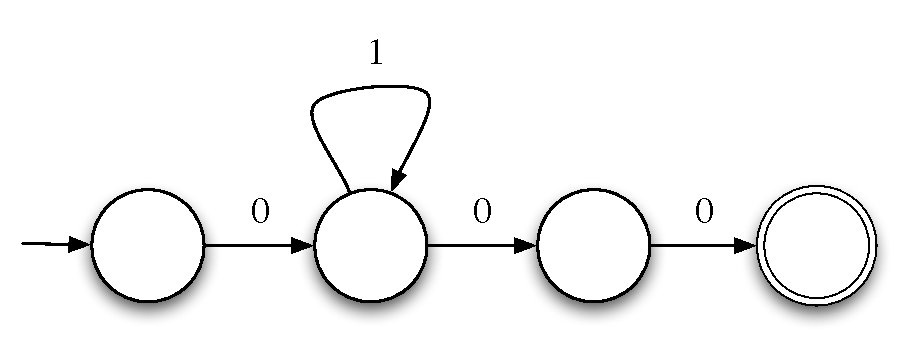
\includegraphics[width=12cm]{figure/finite_automaton.pdf}
 \end{center}
 \caption{有限オートマトン}
 \label{162900_30Mar06}
\end{figure}

直観的には、有限オートマトンはいくつかの{\bfseries 状態}(state)と状態間
の{\bfseries 遷移}(transition)からなる有向グラフで表される(図
\ref{162900_30Mar06})。状態には1つの{\bfseries 初期状態}(initial state)、
複数個の{\bfseries 受理状態}(accepting state)があり、また、各遷移には
アルファベット中の1文字(ラベル)が付けられている。最初、有限オートマトンは初期状態に制御がある。そし
て、入力を1文字読むごとに、入力を現在制御が置かれている状態から伸びる遷移
のラベルと照合し、合致する遷移先の状態に制御を移す。このように状態間の遷
移を繰り返し、入力を読み切ったときに受理状態に制御があれば、その入力を受
理する。図\ref{162900_30Mar06}の有限オートマトンは、0で始まり、次に1が0個
以上続き、00で終わるような記号列をすべて受理する。なお、以下では、
$\epsilon$をラベルに持つ遷移はなく、かつ各状態について、入力となる記号と
照合される遷移は常に1つだけであると仮定する\footnote{すなわち、ここで考え
る有限オートマトンは{\bfseries 決定性}(deterministic)であると仮定す
る。}。

\begin{definition}
 (決定性)有限オートマトン$A$は5つ組$(Q, \Sigma, \delta, q_0, F)$である。
 ここで、
 \begin{itemize}
  \item $Q$:状態の有限集合
  \item $\Sigma$:入力記号の有限集合
  \item $\delta$:遷移関数(transition function)。状態と入力記号を与える
	と状態1つを返す
  \item $q_0 \in Q$:初期状態
  \item $F \subseteq Q$:受理状態の集合
 \end{itemize}$\Box$
\end{definition}

% 有限オートマトンの例

実は、正則表現と有限オートマトンは等価\footnote{任意の正則表現に対して、
その表す言語を受理する有限オートマトンが存在する。また、任意の有限オート
マトンに対して、それが受理する言語を表す正則表現が存在する。}であり、任意
の正則表現から等価な有限オートマトンを構成したり、任意の有限オートマトン
から等価な正則表現を構成することができる。手法の詳細は別の書籍を参照され
たい(例えば\cite{ホップクロフト03:automaton})。この講義で必要になるのは、
極めて簡単な形式の正則表現から有限オートマトンを構成することだけなので、
これについて直観的な説明をするにとどめる。

基本的な正則表現について、対応する有限オートマトンは図
\ref{125936_30Mar06}のようになる。これを再帰的に用いて、有限オートマトン
を順に構成し、最後に初期状態と受理状態を定めればよい。ただし$\epsilon$の
扱いは注意が必要である。$\epsilon\cdot a = a\cdot\epsilon = a$などの性質
を用いて、あらかじめ正則表現から$\epsilon$を除去し、有限オートマトンを構
成しなければならない\footnote{$\epsilon$については、この方法ではうまくい
かない場合があるかもしれない。厳密には、正則表現$\rightarrow$ $\epsilon$
遷移つき非決定性有限オートマトン $\rightarrow$ 非決定性有限オートマトン
$\rightarrow$ 決定性有限オートマトンの順に変換を行わなければならない。詳
細は\cite{ホップクロフト03:automaton}などを参照されたい。}。

\begin{figure}
 \begin{center}
  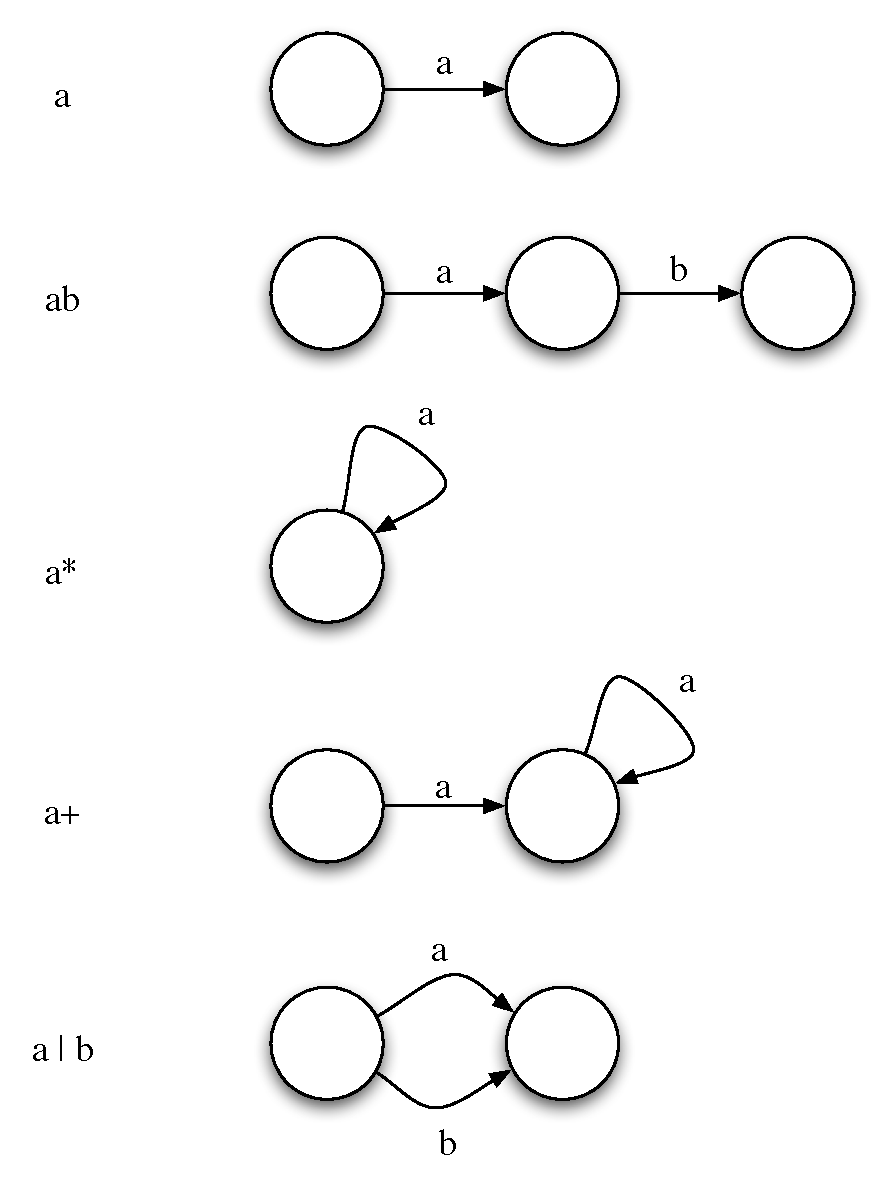
\includegraphics[width=12cm]{figure/regexp_and_fa.pdf}
 \end{center}
 \caption{正則表現と対応する有限オートマトン}
 \label{125936_30Mar06}
\end{figure}

\section{練習問題}

\begin{exercise}
 \label{ex:regexp_01}
 次の言語を表す正則表現を示せ。
 \begin{enumerate}
  \item アルファベット$\{0, 1\}$上の記号列のうち、0から始まり1が0回以上続
	くもの全体からなる言語
  \item アルファベット$\{a, b, c\}$上の記号列のうち、1個以上の$a$と1個以
	上の$b$を含むもの全体からなる言語
  \item アルファベット$\{0, 1\}$上の記号列のうち、0と1が交互に出現するも
	の全体からなる言語
 \end{enumerate}
\end{exercise}
\begin{exercise}
 \label{ex:regexp_02}
 正則表現 $(0 \mid 1)^\ast 0(0\mid 1)(0\mid 1)$ が表す言語は何か。言葉で説明せよ。
\end{exercise}
\begin{exercise}
 \label{ex:regexp_03}
 C言語の空白記号は、空白($_{\sqcup}$)、タブ(\verb|\t|)、改行
 (\verb|\n|)が1個以上並んだ文字列である。これを正則表現で表せ。
\end{exercise}
\begin{exercise}
 \label{ex:regexp_04}
 C言語の16進定数は 0x あるいは 0X で始まり、数字および a, b, c, d, e, f,
 A, B, C, D, E, F が1個以上続く。これを正則表現で表せ。
\end{exercise}
\begin{exercise}
 \label{ex:regexp_05}
 C言語の識別子はA〜Z, a〜z, 0〜9, 下線(\underline{ })からなる文字列であ
 る。ただし、最初の文字に数字を使うことはできない。これを正則表現で表せ。
\end{exercise}
\begin{exercise}
 \label{ex:regexp_06}
 アルファベットを$\{0, 1\}$とするとき、次の言語を受理する有限オートマト
 ンを示せ。
 \begin{enumerate}
  \item $00$で終わる記号列全体
  \item $011$を途中に含む記号列全体
 \end{enumerate}
\end{exercise}
\begin{exercise}
 \label{ex:regexp_07}
 正則表現$00(0 \mid 1)^\ast$に対応する有限オートマトンを構成せよ。
\end{exercise}

%#!platex main

\chapter{字句解析}
\label{103559_30Mar06}

\section{用語}

説明を始める前に、この章を通して用いられる用語を整理しておくことにしよう。

\ref{134201_29Mar06}節で述べたように、字句解析の目的は、文字列としての原
始プログラムから意味のある文字列を切り出すことである。ここで言う「(原始
言語で)意味のある文字列」のことを{\bfseries 字句要素}(lexeme)という。
例えば、C言語の字句要素には次のようなものがある。
\begin{itemize}
 \item 変数名、関数名などの{\bfseries 識別子}(identifier)
 \item \icode{int}, \icode{while}など、C言語プログラム中で特別な意味を持
       ち、他の用途に用いることのできない語({\bfseries 予約語}, keyword)
 \item データの値を表す{\bfseries 定数}(constant)。整数定数、浮動小数点
       定数、文字定数などがある。
 \item 文字列を表す{\bfseries 文字列リテラル}(string literal)
 \item \icode{+}, \icode{*}, \icode{=}, \icode{==}などの{\bfseries 演算
       子}(operator)
 \item 括弧、セミコロンなどの{\bfseries 区切り記号}(separator)
\end{itemize}
空白、タブ、改行文字、コメントなどはC言語のプログラムの意味には影響を与え
ないので、字句解析の際に捨てられる。

実際の字句解析では、切り出した字句要素をそのまま構文解析部に渡すことはせ
ず、字句要素を{\bfseries トークン}(token)というデータに変換してから渡す。
トークンには以下のような情報が含まれる。
\begin{itemize}
 \item 字句要素の種類。例えば\icode{ID}(識別子)、\icode{IF}(予約語
       \icode{if})、\icode{RELOP}(比較演算子)など\footnote{以降、特に
       断らない限り、英大文字と数字からなるゴシック文字列を字句要素の種類
       として用いる。}。
 \item 付加情報。例えば、識別子\icode{argc}には、その識別子の名前、すなわ
       ち ``argc'' が付加情報として付けられる。また整数定数 \icode{453}
       には、その定数の値、すなわち 453 という整数が付加情報として付けら
       れる。付加情報のない場合もある。
\end{itemize}

\section{素朴な字句解析とその問題点}
\label{170323_24Apr06}

字句解析アルゴリズムの前提として、原始プログラムを読む回数は1回に押さえた
い。つまり、原始プログラムのファイルを初めから終わりまで順に1回読み込むだ
けで字句解析を終わらせるようにしたい。これは、CPUの計算に比べて、ファイル
(二次記憶)との入出力はずっと時間がかかるからである。

また、コンパイラ中に巨大な文字配列を確保し、そこに原始プログラムを全部読
み込んでから字句解析をするという方法も好ましくない。巨大な配列を確保する
と、コンパイラの使用メモリ量が増えてしまう。コンパイラは比較的重いプログ
ラムなので、なるべく使用メモリ量を節約して設計したい。

すると、素朴な字句解析プログラムは次のようになるであろう。原始プログラム
ファイルから\icode{getc()}関数で1文字読み、その種類によって場合分けを
行う。これをファイルの終わりまで繰り返す。

\begin{quote}
\begin{lstlisting}[language=C]
 #include <stdio.h>
 /* 後述するように、字句要素は整数で表現する */
 #define IF 1
 /* 以下、字句要素の定義が続く */

 /* 次の字句要素の番号を返す */
 int simple_lexical_analysis()
 {
   char c;
   /* file: 原始プログラムファイル */
   while((c = getc(file)) != EOF) {
     /* 予約語 if の処理 */
     if (c == 'i') {
       c = getc(file);
       if (c == 'f') {
         return IF;
       }
     }
     /* 以下、他の字句要素の処理が続く */
   }
 }
\end{lstlisting}
\end{quote}

しかし、このプログラムには問題がある。字句要素ごとの処理が複雑になってし
まうのである。C言語には、iで始まる予約語は\icode{if}の他に\icode{int}もあ
る。またユーザが i で始まる識別子を使う可能性も高い。このような可能性をす
べて網羅して場合分けを書くのは大変である。ましてやこのプログラムを自動的
に生成するのは難しい。

以下の節では、正則表現を用いて字句解析部を自動的に生成する手法を述べる。

\section{正則表現を基にした字句解析}
\label{112953_24Apr06}

\begin{figure}
 \begin{center}
  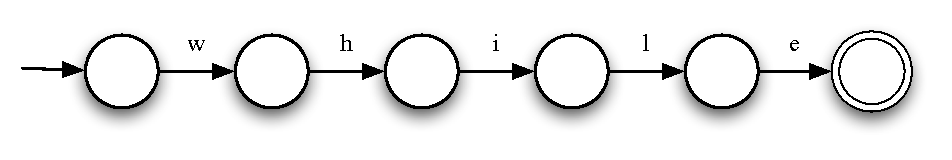
\includegraphics[width=13cm]{figure/fa_while.pdf}
 \end{center}
 \caption{\icode{while}に対応する有限オートマトン}
 \label{163948_18Apr06}
\end{figure}
\begin{figure}
 \begin{center}
  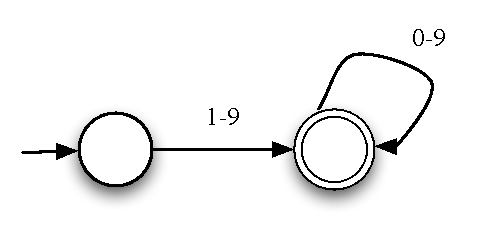
\includegraphics{figure/fa_decimal.pdf}
 \end{center}
 \caption{10進数に対応する有限オートマトン}
 \label{164232_18Apr06}
\end{figure}

字句解析の手法では、次のことを考える必要がある。
\begin{enumerate}
 \item 字句要素を定義する方法
       \label{075512_23Apr08}
 \item \ref{075512_23Apr08} で定義した字句要素を検出する方法
       \label{075846_23Apr08}
 \item 字句要素を検出したときに何らかの動作を行う方法(整数定数の字句要
       素を検出したときにその整数の値を求める、など)
\end{enumerate}

ここで述べる字句解析手法では、各字句要素を正則表現で表し、対応する有限オートマトン
を構成して字句要素を受理させる。上に述べた\ref{075512_23Apr08} の実現方法
として正則表現を、\ref{075846_23Apr08} の実現方法として有限オートマトン
を利用するのである。例えば、予約語
\icode{while}に対応する正則表現は$while$であり、この正則表現と等価な有限
オートマトンは図\ref{163948_18Apr06}のようになる。また、C言語の10進定数は
0以外の数字から始まる数字の列であるので、これに対応する正則表現は
$[1\mbox{-}9][0\mbox{-}9]^\ast$であり、これと等価な有限オートマトンは図
\ref{164232_18Apr06}のようになる。

このような有限オートマトンをすべての字句要素に対して作り、並列に動作させ
る。つまり、原始プログラムファイルから1文字読み込んで、それを入力記号とし
てすべての有限オートマトンを動作させる。これを繰り返して、ある有限オート
マトンが受理状態に到達すれば、字句要素が見つかったことになる。例えば
`w', `h', `i', `l', `e' の順に原始プログラムファイルから文字を読み込んだ
とすると、図\ref{163948_18Apr06}の有限オートマトンは受理状態に到達し、一
方、それ以外の有限オートマトン(例えば図\ref{164232_18Apr06}のオートマト
ン)は受理状態に到達しない。従って、字句要素\icode{while}が見つかったこと
になる。字句要素が1つ見つかれば、すべての有限オートマトンをリセットし(初
期状態に戻して)、再び原始プログラムファイルからの文字の読込みを始める。

ただし、この方法ではまだ問題点が残っている。
\begin{figure}
 \begin{center}
  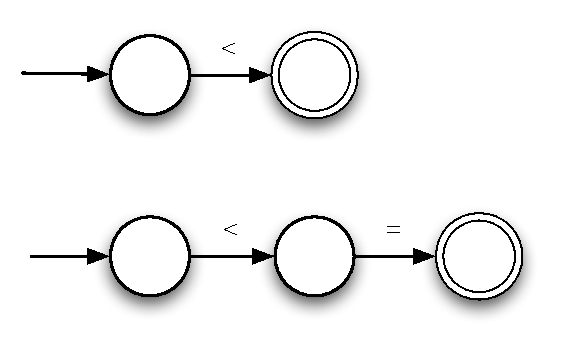
\includegraphics{figure/fa_relop.pdf}
 \end{center}
 \caption{比較演算子に対する有限オートマトン}
 \label{182549_18Apr06}
\end{figure}
\begin{figure}
 \begin{center}
  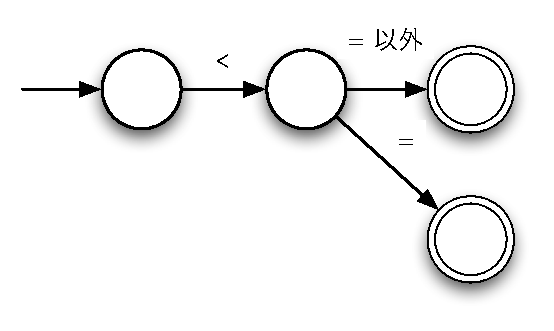
\includegraphics{figure/fa_relop_fixed.pdf}
 \end{center}
 \caption{比較演算子に対する有限オートマトン(改良版)}
 \label{183745_18Apr06}
\end{figure}
\begin{figure}
 \begin{center}
  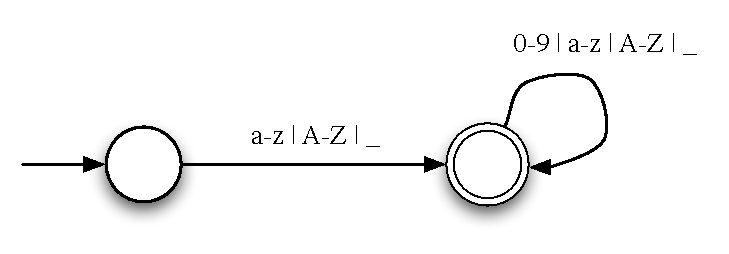
\includegraphics{figure/fa_identifier.pdf}
 \end{center}
 \caption{識別子に対する有限オートマトン}
 \label{081246_19Apr06}
\end{figure}
\begin{enumerate}
 \item 一つの文字列が2つ以上の有限オートマトンで受理されることがある。例
       えば文字列 `while' は図\ref{163948_18Apr06}の有限オートマトンで受
       理されるが、C言語の識別子を受理する有限オートマトン(図
       \ref{081246_19Apr06}、練習問題\ref{ex:regexp_05}を参照)でも受理さ
       れる。この場合、C言語では予約語として解釈しなければならない。すな
       わち、図\ref{163948_18Apr06}の有限オートマトンを優先して処理しなけ
       ればならない。
 \item (最長一致の原則) 字句要素を認識するときは、最も長いものを採用しな
       ければならない。例えば\verb|<|と\verb|<=|という2つの字句要素を考え
       よう。これらの字句要素を受理する有限オートマトンを図
       \ref{182549_18Apr06}に示す。`\verb|<|'を読み込んだとき、上のオート
       マトンは受理状態に到達する。しかし、もしこの次の文字が `\verb|=|'
       であれば、\verb|<|ではなく\verb|<=|という字句要素と解釈しなければ
       ならない。つまり、下のオートマトンのみで受理させなければならない。
       \label{183630_18Apr06}
\end{enumerate}

\ref{183630_18Apr06}に挙げた図\ref{182549_18Apr06}の問題点を改良する一つ
の案を図\ref{183745_18Apr06}に示す。ポイントは、`\verb|<|'を受理する有限オー
トマトンを改良し、`\verb|<|'の次に `=' 以外の文字を読み込んだときに受理す
る、とした点である。一般に、最長一致の原則はこれと同様の方法で解決できる。

ただし、注意しなければならない点がある。上のオートマトンで字句要素
`\verb|<|'を受理したとき、本来の字句要素`\verb|<|'よりも1文字余計に読み込
んでしまっている。この余計に読み込んだ文字は、次の字句要素を構成する文字
であるかもしれないため、`\verb|<|'を受理した後、読み込みを破棄しておかな
ければならない。

\section{字句解析プログラムの実現}
\label{170501_24Apr06}

\begin{figure}
 \begin{center}
  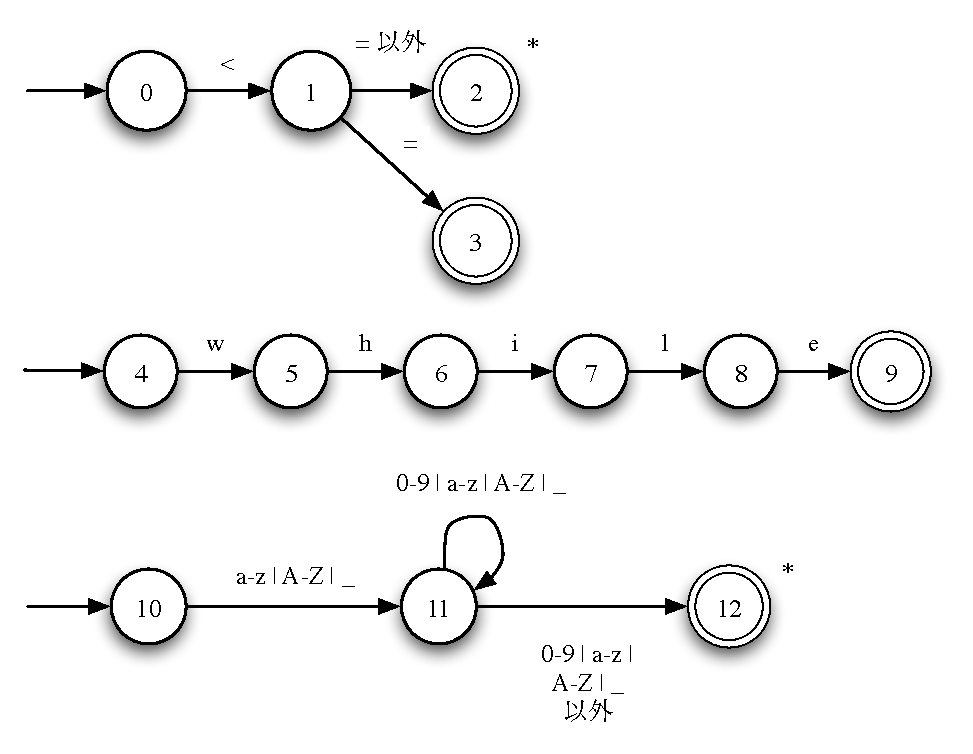
\includegraphics[width=13cm]{figure/lexical_analysis_example.pdf}
 \end{center}
 \caption{字句解析のための有限オートマトン群}
 \label{112450_24Apr06}
\end{figure}

有限オートマトンを基礎とする字句解析プログラムの実現について説明を行う。
なお、説明のため、ここでは認識すべきトークンを\verb|<|, \verb|<=|,
\icode{while}, それにC言語の識別子のみとする。また、これらのトークンを認
識する有限オートマトンの状態に番号を付けておく(図\ref{112450_24Apr06})。

\subsection{ファイルとの入出力}

これから作成する字句解析プログラムは、原始プログラムファイルから1文字ずつ
文字を読み、処理する、という操作をファイルの終わりまで繰り返す。ただし、
\ref{112953_24Apr06}節で述べたように、字句によっては、字句を認識した後に読
み込みを破棄しておかなければならない。

したがって、原始プログラムファイルからの読み込みは\icode{getc()}関数を、
読み込みの破棄は\icode{ungetc()}関数をそれぞれ用いればよい
\footnote{\icode{ungetc()}関数は今まで使ったことがないと思われるので、オ
ンラインマニュアルなどでどういう関数か調べておくこと。\icode{getc()}関数
を知らない、もしくは忘れている場合もオンラインマニュアルなどで調べておく
こと。}。ただし、この部分は後で改良を試みたいので、直接\icode{getc()},
\icode{ungetc()}を使うのではなく、次のような関数を通して使うことにする。

\begin{lstlisting}
 int nextchar(FILE* infile)
 {
    return getc(infile);
 }

 void backchar(int c, FILE* infile)
 {
    ungetc(c, infile);
 }
\end{lstlisting}

\subsection{データの表現}

コンパイラでは通常、原始言語のトークンに通し番号を付け、コンパイラの内部
でもその番号(整数)でそれぞれのトークンを表す。次の例では、
\verb|<|, \verb|<=|, \icode{while}, 識別子にそれぞれ 0, 1, 2, 3 という番
号を割り当てている。

\begin{lstlisting}
 #define LT  0
 #define LE  1
 #define WHILE 2
 #define ID  3
\end{lstlisting}

すると次節で示すように、字句解析プログラムはトークンを表す番号を返り値と
する関数となり、したがって\icode{int}型の値を返す関数となる。

ただし識別子については、実際の識別子名(\icode{i}, \icode{main}などの変数
名や関数名)も字句解析の出力とする必要がある。これは大域変数\icode{char~%
yytext[80];}に格納されるものとする\footnote{字句解析部の後に続く構文解析
部から識別子名を参照できるように、大域変数を用いている。}。

字句解析プログラムでは、ほかに次のような大域変数を用いる。
\begin{itemize}
 \item \icode{int state;}…有限オートマトンの現在の状態を表す。初期値は0。
 \item \icode{int initial\_state;}…現在処理中の有限オートマトンの初期状態
       を表す。初期値は0。
 \item \icode{FILE *file;}…原始プログラムのファイルポインタ。
\end{itemize}

\subsection{字句解析プログラム}

次に、字句解析プログラムの本体である\icode{nexttoken()}関数のコードを示す。
この関数は、構文解析部から必要に応じて呼び出されることを想定しており、次
のトークンを表す番号を返り値とする。また、トークンが識別子の場合には、大
域変数\icode{yytext}にその識別子名を格納する。

\begin{quote}
 \lstinputlisting[numbers=left]{code/nexttoken.c}
\end{quote}

大まかには、現在の状態(\icode{state})と次の文字(\icode{c})から次の状
態を決定し、\icode{state}の値を更新し、状態による分岐を行う(35行目)。そ
の結果受理状態に到達すれば、認識したトークンの番号を返す。受理状態に到達
できなかった場合は、\icode{fail()}関数を呼び出し、初期状態\icode{start}の
値を更新して次のオートマトンによる受理を試す。これをオートマトンの数だけ
繰り返していく。どのオートマトンでも受理できなかった場合は、原始プログラ
ムに誤りがあったことになるので、エラー処理を行う
\footnote{\icode{isalpha(c)}関数、\icode{isdigit(c)}関数はそれぞれ、
\icode{c}がアルファベットか、\icode{c}が数字かを判定する関数である。詳細
はオンラインマニュアルなどを参照のこと。}。

図\ref{112450_24Apr06}で$\ast$を付けた状態は、認識したトークンよりも1文字
先まで読み込んでしまっていることを示す。例えばトークン `\verb|<|'は、トー
クンの読み込み自体は状態1で終了しているが、`\verb|<|'か`\verb|<=|'かを決
定するために1文字先まで読み込み、状態2に至る必要がある。識別子も、識別子
に含まれない文字が出てきた時点で初めて、識別子の終わりが認識できるため、
状態12 に到達したときには1文字先まで読んでしまっていることになる。そのた
め、状態2と状態12については、\icode{backchar()}関数により、1文字分読み込
みを破棄している。

入力の破棄はオートマトンを切り替える際にも発生する。例えば状態6で、文字
`a'を読み込んでトークン\icode{while}の認識に失敗した場合、すでに読み込ん
だ `w', `h', `a'を破棄してから次のオートマトンに切り替えなければならない。
そのために、既に読み込んだ文字を蓄える配列\icode{s}、読み込んだ文字数を保
持する変数\icode{i}を局所変数として用意している。\icode{fail()}を呼び出す
ときには\icode{s}と\icode{i}を引数として渡し、\icode{fail()}中で入力の破
棄を行っている。

また状態12では、現在の\icode{s}の内容、すなわち認識した識別子名を大域変数
\icode{yytext}にコピーしている。

\subsection{字句解析部自動生成プログラム\icode{lex}}

\ref{170501_24Apr06}節で示した字句解析プログラムは各状態で行うべき処理が
かなりパターン化されており、図\ref{112450_24Apr06}のオートマトンが与えら
れれば、\ref{170323_24Apr06}節で示したプログラムに比べて自動的に生成しや
すい。

実は、字句解析部を自動生成するプログラムはいくつもある。これらはいずれも、
認識すべきトークンの正則表現と、トークンに対して行うべき処理を指定すると、
字句解析プログラムを自動生成してくれる。内部的には、正則表現から図
\ref{112450_24Apr06}に相当するオートマトンを自動生成し(アルゴリズムは例
えば\cite{ホップクロフト03:automaton}を参照)、さらに
\ref{170501_24Apr06}節に示したような字句解析プログラムを自動生成している。

例として、Unixに標準装備されている\icode{lex}プログラムを取り上げる。
\ref{170501_24Apr06}節のプログラムと同等の字句解析プログラムを自動生成す
るには、以下のようなルールを書き、\icode{lex}で処理すればよい。

\begin{quote}
 \lstinputlisting{code/nexttoken.lex}
\end{quote}

`\verb|%{|'から `\verb|%}|'までがトークンの番号指定、`\verb|%%|'に挟まれ
た部分が認識すべきトークンを表す正則表現と、そのときに行われる処理(C言語
プログラム)である。識別子名は自動的に\icode{yytext}という変数に格納され
る。

\icode{lex}やその他の字句解析部自動生成ソフトウェアの詳細は、ここでは省略
する。各自で適宜参考資料にあたられたい。

\section{入力のバッファリング}

本章の最後に、\icode{nextchar()}関数、\icode{backchar()}関数の改良につい
て考えよう。

\begin{figure}
 \begin{center}
  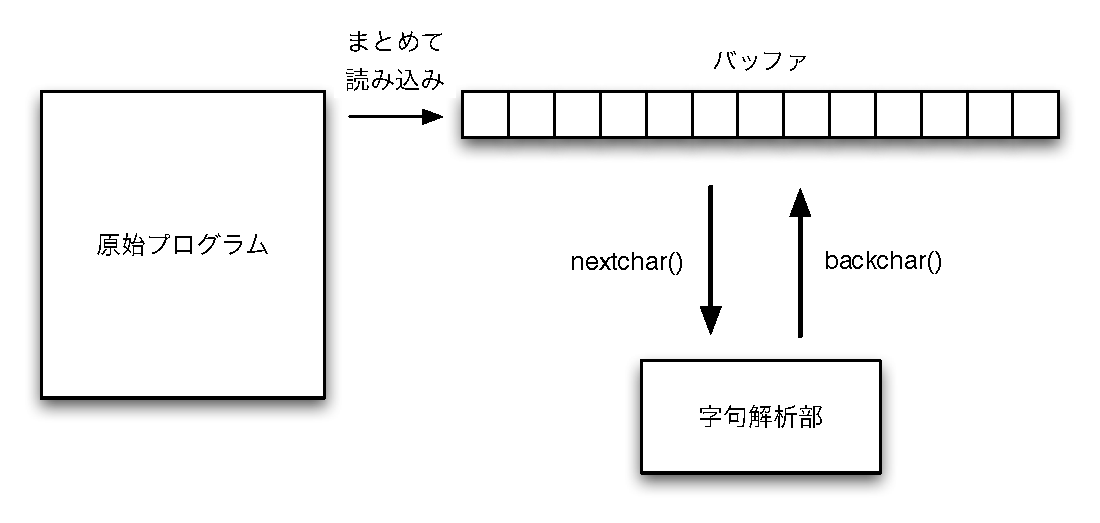
\includegraphics[width=13cm]{figure/buffering.pdf}
 \end{center}
 \caption{入力のバッファリング}
 \label{175102_24Apr06}
\end{figure}

基本となる考え方は、プログラム中に{\bfseries バッファ}(buffer)と呼ばれ
る領域を用意しておく、というものである。あらかじめ、原始プログラムから一
定量の文字をバッファに取り込んでおき、\icode{nextchar()}と
\icode{backchar()}はバッファから1文字読み込んだり、バッファに文字を戻した
りするようにする(図\ref{175102_24Apr06})。これにより、\icode{ungetc()}
関数を使う必要はなくなる\footnote{本章の例では示していないが、原始プログ
ラムからバッファへの読み込みも、\icode{getc()}を用いて1文字ずつ読み込むの
ではなく、\icode{gets()}などにより複数の文字をまとめて読み込むことができ、
やはり効率が良くなる。}。

バッファを用いた改良版\icode{nextchar()}、\icode{backchar()}を次に示す。
この例では、長さ2048のバッファ(\icode{char}型の配列)を用意し、前半分と
後ろ半分を交互に用いている。変数\icode{forward}は大域変数で、現在処理して
いる文字の添字を保持している。

\begin{quote}
 \lstinputlisting{code/nextchar.c}
\end{quote}

字句解析部でバッファを用いると、入力の破棄に関してもう一つ利点が生まれる。
\ref{170501_24Apr06}節の字句解析プログラムでは、\icode{backchar()}の呼び
出しが発生したときに備え、現在処理中の文字列を\icode{nexttoken()}中に保持
しておく必要があった(変数\icode{s})。しかし、バッファを用いると、現在処
理中の文字列は必ずバッファ中に残っている。これを利用すると、現在処理中の
文字列を\icode{nexttoken()}中で保持しておく必要がなくなる。改良版の
\icode{nexttoken()}、\icode{fail()}を次に示す。変数\icode{beginning}は、
現在処理しているオートマトンが初期状態であったときの\icode{forward}の位置、
すなわち現在処理中のトークンの先頭の添字を保持している。

\begin{quote}
 \lstinputlisting{code/nexttoken_buffer.c}
\end{quote}

%#!platex main

\chapter{$BJ8L.<+M3J8K!(B}
\label{151253_30Mar06}

$B9=J82r@OIt$N=hM}$G$O!"2?$i$+$N7A$G86;O%W%m%0%i%`8@8l$N9=J8$r%3%s%T%e!<%?(B
$B$G07$o$J$1$l$P$J$i$J$$!#(B\ref{175712_30Mar06}$B>O$G<h$j>e$2$?@5B'I=8=$O!"86(B
$B;O%W%m%0%i%`8@8l$G07$&;z6gMWAG$rDj5A$9$k$3$H$O$G$-$k$,!"$=$l$i$r$I$N$h$&(B
$B$KAH$_9g$o$;$l$PJ8K!E*$K@5$7$$$N$+!"$K$D$$$F$ODj5A$9$k$3$H$,$G$-$J$$!#(B

$BK\>O$G$O!"%W%m%0%i%_%s%08@8l$N9=J8$r07$&$?$a$N4pK\E*$JM}O@$G$"$kJ8L.<+M3(B
$BJ8K!$K$D$$$F@bL@$7!"9=J82r@O$KI,MW$J$$$/$D$+$N=EMW$J@-<A$K$D$$$F=R$Y$k!#(B

$B$J$*!"K\>O$G$b(B\ref{175712_30Mar06}$B>O$G=R$Y$?8@8lM}O@$K4X$9$kMQ8l$rMQ$$$k!#(B

\section{$BJ8L.<+M3J8K!(B}

\subsection{$BDj5A(B}

$B%W%m%0%i%_%s%08@8l$N9=J8$rDj5A$9$k$K$O!"DL>o!"(B{\bfseries $BJ8L.<+M3J8(B
$BK!(B}$B!J(Bcontext free grammar$B!K$rMQ$$$k!#Nc$($P(BC$B8@8l$N(Bif$BJ8$N9=J8$O!"(B
$BJ8L.<+M3J8K!$G$O<!$N$h$&$K=q$/$3$H$,$G$-$k!#(B
\begin{align*}
 selection\_statement & \rightarrow {\sf if}\ {\sf (}\ expression\ 
  {\sf )}\ statement \\
 selection\_statement & \rightarrow {\sf if}\ {\sf (}\ expression\ 
  {\sf )}\ statement\ 
 {\sf else}\ statement\ 
\end{align*}

$BLp0u(B$\rightarrow$$B$H$=$NN>JU$+$i$J$k<0$r(B{\bfseries $B@8@.5,B'(B}$B!J(Bproduction
rule$B!K!"$b$7$/$ON,$7$F(B{\bfseries $B5,B'(B}$B!J(Brule$B!K$H$$$&!#@8@.5,B'$N:8JU$O5-(B
$B9f(B1$B$D!"1&JU$O5-9fNs$+$i@.$C$F$$$k!#5-9f$O(B{\bfseries $BHs=*C<5-(B
$B9f(B}$B!J(Bnonterminal symbol$B!K$H(B{\bfseries $B=*C<5-9f(B}$B!J(Bterminal symbol$B!K$KJ,$1(B
$B$i$l$k!#$3$NNc$G$O!"(B$selection\_statement$, $expression$, $statement$$B$,Hs(B
$B=*C<5-9f!"(B{\sf if}, {\sf (}, {\sf )}, {\sf else}$B$,=*C<5-9f$G$"$k!#@8@.5,(B
$BB'$N:8JU$K$OHs=*C<5-9f$7$+=P8=$G$-$J$$!#1&JU$K$OHs=*C<5-9f!"=*C<5-9f$H$b(B
$B$K=P8=$9$k$3$H$,$G$-$k!#Hs=*C<5-9f$N$&$A(B1$B$D$rFC$K(B{\bfseries $B3+;O5-(B
$B9f(B}$B!J(Bstart symbol$B!K$H$$$&!#(B

$B$b$&(B1$B$DNc$H$7$F!V?t;z!"(B$+$$B!"(B$-$$B$+$i$J$k<0!W$rI=$9J8L.<+M3J8K!$r<($=$&!#(B
\begin{equation}
 \begin{split}
 list & \rightarrow list\ {\sf +}\ digit \\
 list & \rightarrow list\ {\sf -}\ digit \\
 list & \rightarrow digit \\
 digit & \rightarrow {\sf 0} \mid {\sf 1} \mid {\sf 2} \mid {\sf 3}
  \mid {\sf 4} \mid {\sf 5} \mid {\sf 6} \mid
  {\sf 7} \mid {\sf 8} \mid {\sf 9}
 \end{split}\label{171007_30Mar06}
\end{equation}

$B$3$NNc$G$O(B$list$, $digit$$B$,Hs=*C<5-9f!"?t;z$H(B${\sf +}$, ${\sf -}$$B$,=*C<5-(B
$B9f$G$"$k!#$^$?!":G8e$N5,B'$N(B$\mid$$B$O!V$^$?$O!W$N0UL#$G$"$k!#$J$*!"$3$NNc(B
$B$+$iJ,$+$k$h$&$K!":8JU$NHs=*C<5-9f$,F1$8@8@.5,B'$N1&JU$K=P8=$7$F$b$+$^$o(B
$B$J$$!#(B

$B$^$H$a$k$H!"J8L.<+M3J8K!(B$G$$B$O<!$N$h$&$J9=@.MWAG$+$i$J$k!#(B
\begin{enumerate}
 \item $BHs=*C<5-9f$NM-8B=89g(B$V$
 \item $B=*C<5-9f$NM-8B=89g(B$T$
 \item $B@8@.5,B'$NM-8B=89g(B$P$
 \item $B3+;O5-9f(B$S \in V$$B!#Hs=*C<5-9f$N$&$A(B1$B$D(B
\end{enumerate}

$B5-9f$r(B1$B$D$b4^$^$J$$Ns$b$"$k!#$3$l$r(B{\bfseries $B6uNs(B}$B!J(Bempty string$B!K$H$h$S!"(B
$\epsilon$$B$H$$$&5-9f$GI=$9!#$^$?!"%W%m%0%i%_%s%08@8l$N9=J8$rI=$9I=8=$H$7(B
$B$F!"$[$+$K(B{\bfseries BNF $B5-K!(B}$B!J(BBackus Naur Form$B!K$H$$$&$b$N$,$"$k$,!"J8(B
$BL.<+M3J8K!$H$[$\F1$8$H9M$($F$h$$!#(BBNF$B5-K!$G>e$NJ8K!$r=q$/$H<!$N$h$&$K$J$k!#(B
\begin{align*}
 list & ::= list + digit \\
 list & ::= list - digit \\
 list & ::= digit \\
 digit & ::= 0 \mid 1 \mid 2 \mid 3 \mid 4 \mid 5 \mid 6 \mid 7 \mid 8
 \mid 9 
\end{align*}

% \begin{example}
%  $B<!$NJ8K!$O!"4JC1$J;;=Q<0$rDj5A$9$k$b$N$G$"$k!#(B
%  \begin{eqnarray*}
%   expr & \rightarrow & expr\ op\ expr \mid (\ expr\ )\mid -\ expr\mid
%    {\bf id} \\
%   op & \rightarrow & + \mid - \mid * \mid / 
%  \end{eqnarray*}$\Box$
% \end{example}

$B0J9_$N@bL@$G$O!"<!$N$h$&$K5-K!$r7h$a$F$*$/$3$H$K$9$k!#(B
\begin{enumerate}
 \item $BA0$N$[$&$N1Q>.J8;z(B($a, b, c, \cdots$)$B!"1i;;;R5-9f(B($+, -, \cdots$)$B!"(B
       $B3g8L$d%3%s%^$J$I$N6h@Z$j5-9f!"?t;z!"B@;z$N5-9fNs$O=*C<5-9f$rI=$9!#(B
 \item $BA0$N$[$&$N1QBgJ8;z(B($A, B, C, \cdots$)$B!"(B$S$ ($B3+;O5-9f(B)$B!"1Q>.J8;z$N(B
       $B%$%?%j%C%/BN$NL>A0(B({\itshape expr}, {\itshape stmt}$B$J$I(B)$B$OHs=*C<5-(B
       $B9f$rI=$9!#(B
 \item $B8e$m$N$[$&$N1QBgJ8;z(B($X, Y, Z, \cdots$)$B$OHs=*C<5-9f$^$?$O=*C<5-9f(B
       $B$rI=$9!#(B
 \item $B8e$m$N$[$&$N1Q>.J8;z(B($w, x, y, z, \cdots$)$B$O=*C<5-9fNs$rI=$9!#(B
 \item $B>.J8;z$N%.%j%7%cJ8;z(B($\alpha, \beta, \gamma, \cdots$)$B$O!"5-9fNs(B($B=*(B
       $BC<5-9f$HHs=*C<5-9f$,:.$6$C$F$$$F$h$$(B)$B$rI=$9!#(B
 \item $B:G=i$K8=$l$k@8@.5,B'$N:8JU$r3+;O5-9f$H$9$k!#$^$?!"(B$S$$B$r3+;O5-9f$H(B
       $B$9$k$3$H$,B?$$!#(B
\end{enumerate}

\subsection{$BJ8L.<+M3J8K!$N0UL#(B}

$BJ8L.<+M3J8K!(B$G = (V, T, P, S)$$B$O!"(B$T$$B!"$9$J$o$A=*C<5-9f$N=89g$r%"%k%U%!%Y%C(B
$B%H$H$9$k8@8l$rI=$7$F$$$k!#$G$O!"6qBNE*$K$I$N$h$&$J8@8l$rI=$7$F$$$k$N$@$m(B
$B$&$+!#(B

$BJ8K!$N8@8l$NDj5AJ}K!$K$O$$$/$D$+$"$k$,!"$=$N(B1$B$D$K!V@8@.5,B'$r=q$-49$(5,B'(B
$B$H9M$($k!W$H$$$&$b$N$,$"$k!#$D$^$j!"3+;O5-9f(B$S$$B$r(B$S$-$B@8@.5,B'$N1&JU$N5-9f(B
$BNs(B$\alpha$$B$GCV$-49$(!"$5$i$K(B$\alpha$$B$K4^$^$l$kHs=*C<5-9f$r!"$=$N5-9f$N@8(B
$B@.5,B'$N1&JU$GCV$-49$($k!#$3$NA`:n$r!"5-9fNs$,=*C<5-9f$N$_$K$J$k$^$G7+$j(B
$BJV$9!#$3$N$h$&$K$7$FF@$i$l$k=*C<5-9fNs$9$Y$F$N=89g$r!"$=$NJ8K!$N(B
{\bfseries $B8@8l(B}$B!J(Blanguage$B!K$H$$$&!#(B

\begin{example}
 \eqref{171007_30Mar06}$B$NJ8K!(B
 \begin{align}
  list & \rightarrow list\ {\sf +}\ digit\label{171930_30Mar06} \\
  list & \rightarrow list\ {\sf -}\ digit\label{172048_30Mar06} \\
  list & \rightarrow digit\label{172152_30Mar06} \\
  digit & \rightarrow {\sf 0} \mid {\sf 1} \mid {\sf 2} \mid {\sf 3}
  \mid {\sf 4} \mid {\sf 5} \mid {\sf 6} \mid
  {\sf 7} \mid {\sf 8} \mid {\sf 9}\label{172302_30Mar06}
 \end{align}
 $B$K$D$$$F!"(B\eqref{171930_30Mar06}$B$rMQ$$$k$H!"3+;O5-9f(B$list$$B$r1&JU$N5-9fNs(B
 $list + digit$$B$KCV$-49$($k$3$H$,$G$-$k!#$3$l$r7+$jJV$9$H!"0J2<$N$h$&$K=*(B
 $BC<5-9fNs(B$9-5+2$$B$rF@$k$3$H$,$G$-$k!#(B
 \begin{align*}
  \underline{list} & \Rightarrow \underline{list} + digit &&
  \text{\eqref{171930_30Mar06}$B$rE,MQ(B} \\
       & \Rightarrow \underline{list} - digit + digit &&
  \text{\eqref{172048_30Mar06}$B$rE,MQ(B} \\
       & \Rightarrow \underline{digit} - digit + digit &&
  \text{\eqref{172152_30Mar06}$B$rE,MQ(B} \\ 
       & \Rightarrow 9 - \underline{digit} + digit && \text{\eqref{172302_30Mar06}$B$r(B
  $BE,MQ(B} \\
       & \Rightarrow 9 - 5 + \underline{digit} && \text{\eqref{172302_30Mar06}$B$rE,MQ(B} \\
       & \Rightarrow 9 - 5 + 2 && \text{\eqref{172302_30Mar06}$B$rE,MQ(B}
 \end{align*}
\end{example}

$B$b$&>/$77A<0E*$K=q$/$H<!$N$h$&$K$J$k!#@8@.5,B'(B$A \rightarrow \gamma$$B$r5-(B
$B9fNs(B$\alpha A\beta$$B$KE,MQ$7$F(B$A$$B$r(B$\gamma$$B$KCV$-49$($k$H(B
$\alpha\gamma\beta$$B$H$J$k!#$3$N$H$-!"(B$\alpha A\beta$$B$+$i(B
$\alpha\gamma\beta$$B$,(B{\bfseries $BF3=P$5$l$k(B}$B!J(Bderive$B!K$H$$$$!"(B$\alpha
A\beta \Rightarrow \alpha\gamma\beta$$B$HI=$9!#(B$\alpha_1$$B$K(B0$B2s0J>eCV$-49$((B
$B$rE,MQ$7$F(B$\alpha_n$$B$,F3=P$5$l$k$H$-!"(B$\alpha_1
\stackrel{*}{\Rightarrow} \alpha_n$$B$H=q$/!#(B
$S \stackrel{*}{\Rightarrow} \alpha$$B$N$H$-!"(B$\alpha$$B$r(B{\bfseries $BJ87A<0(B}
$B!J(Bsentential form$B!K$H$$$&!#$H$/$K(B$\alpha$$B$,=*C<5-9f$N$_$+$i$J$k$H$-!"(B
{\bfseries $BJ8(B}$B!J(Bsentence$B!K$H$$$&!#(B

$BJ8K!(B$G$$B$N8@8l(B$L(G)$$B$H$O!"(B$L(G) = \{w \mid S \stackrel{*}{\Rightarrow}
w\}$$B$G$"$k!#$?$@$7(B$S$$B$O(B$G$$B$N3+;O5-9f$G$"$k!#$9$J$o$A!"(B$G$$B$N8@8l$H$O!"(B
$G$$B$N3+;O5-9f$+$iF3=P$5$l$kJ8$N=89g$G$"$k!#(B


\section{$B2r@OLZ$HF3=P(B}

$BJ8L.<+M3J8K!$N3+;O5-9f$K$I$N$h$&$K@8@.5,B'$,E,MQ$5$l!"=*C<5-9fNs$,@8@.$5(B
$B$l$?$N$+$r?^<($7$?$b$N$r(B{\bfseries $B2r@OLZ(B}$B!J(Bparse tree$B!K$H$$$&!#2r@OLZ$O!"(B
$BF3=P$NMM;R$r?^<($7$?$b$N$G$"$k$H9M$($i$l!"J8$N(B ``$B9=J8E*$J9=B$(B''$B$rI=$7$?$b(B
$B$N$@$H8@$($k!#Nc$($P!"(B\eqref{171007_30Mar06}$B$K<($7$?J8L.<+M3J8K!$K$D$$$F!"(B
$B<0(B$9-5+2$$B$N2r@OLZ$O?^(B\ref{152653_30Mar06}$B$N$h$&$K$J$k!#(B

\begin{figure}
 \begin{center}
  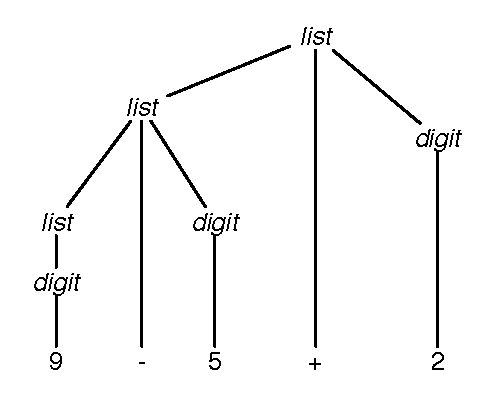
\includegraphics{figure/parse_tree_01.pdf}
 \end{center}
 \caption{$B2r@OLZ$NNc(B}
 \label{152653_30Mar06}
\end{figure}

$B7A<0E*$K$O!"2r@OLZ$O<!$N$h$&$JLZ$G$"$k!#(B
\begin{enumerate}
 \item $B:,$O3+;O5-9f$r%i%Y%k$H$7$F;}$D!#(B
 \item $BMU$O=*C<5-9f$^$?$O(B$\epsilon$$B$r%i%Y%k$H$7$F;}$D!#(B
 \item $BFbIt$N@a$OHs=*C<5-9f$r%i%Y%k$H$7$F;}$D!#(B
 \item $BHs=*C<5-9f(BA$B$r%i%Y%k$K;}$DFbIt$N@a$N;R$,:8$+$i=g$K(B$X_1, X_2,
       \cdots, X_n$$B$H$9$k$H!"(B$A \rightarrow X_1 X_2 \cdots X_n$$B$O@8@.5,B'(B
       $B$G$"$k!#(B$A \rightarrow \epsilon$$B$KBP$7$F$O!"@a(B$A$$B$O(B$\epsilon$$B$r%i(B
       $B%Y%k$H$9$k;R$r;}$D!#(B
\end{enumerate}

$B2r@OLZ$NMU$r:8$+$i1&$KFI$s$G$$$/$H!"=*C<5-9fNs$,F@$i$l$k!#$3$l$,3+;O5-9f(B
$B$+$i@8@.$5$l$k=*C<5-9fNs!"$9$J$o$AJ8$G$"$k!#$3$l$r2r@OLZ$N(B{\bfseries $B7k(B
$B2L(B}$B!J(Bresult$B!K$H$$$&!#(B

\subsection{$B2r@OLZ$N0U5A(B}

$B2r@OLZ$O!"<0$NCM$r7W;;$7$?$j%W%m%0%i%`$rK]Lu$9$k:]$K$$$m$$$mLrN)$D!#Nc$((B
$B$P!"@h$K=R$Y$??t<0$NCM$r7W;;$9$k$3$H$r9M$($h$&!#3FHs=*C<5-9f$,B0@-(B$v$$B$r;}(B
$B$A!"3F@8@.5,B'$K<!$N$h$&$J%W%m%0%i%`JR$,IU$1$i$l$F$$$k$H$9$k!#$J$*!":8JU(B
$B$H1&JU$KF1$8Hs=*C<5-9f$,=P8=$9$k>l9g$K$O!"JX59>e!"$=$l$>$l(B$l$$B$H(B$r$$B$H$$$&(B
$BE:;z$rIU$1$F6hJL$7$F$$$k!#(B
\begin{align*}
 list & \rightarrow list + digit \quad \{ list_l.v = list_r.v + digit.v; \} \\
 list & \rightarrow list - digit \quad \{ list_l.v = list_r.v - digit.v; \} \\
 list & \rightarrow digit \quad \{ list.v = digit.v; \} \\
 digit & \rightarrow 0	\quad \{ digit.v = 0; \} \\
 digit & \rightarrow 1	\quad \{ digit.v = 1; \} \\
 \cdots \\
 digit & \rightarrow 9 \quad \{ digit.v = 9; \} \\
\end{align*}

$B2r@OLZ$N@aE@$NB0@-(B$v$$B$NCM$r!"$=$N@aE@$KBP1~$9$k@8@.5,B'$KIU$1$i$l$?%W%m%0(B
$B%i%`JR$K4p$E$$$F7W;;$9$k$H!"$=$N2r@OLZ$N7k2L$G$"$k<0$NCM$,5a$a$i$l$k!#<0(B
$9 - 5 + 2$$B$N2r@OLZ$K$h$kNc$r?^(B\ref{190545_30Mar06}$B$K<($9!#$3$N7W;;$O!"2r(B
$B@OLZ$r?<$5M%@h$GC5:w$7!"5"$j$,$1$K%W%m%0%i%`JR$r<B9T$9$k$3$H$KAjEv$7$F$$(B
$B$k!#(B

\begin{figure}
 \begin{center}
  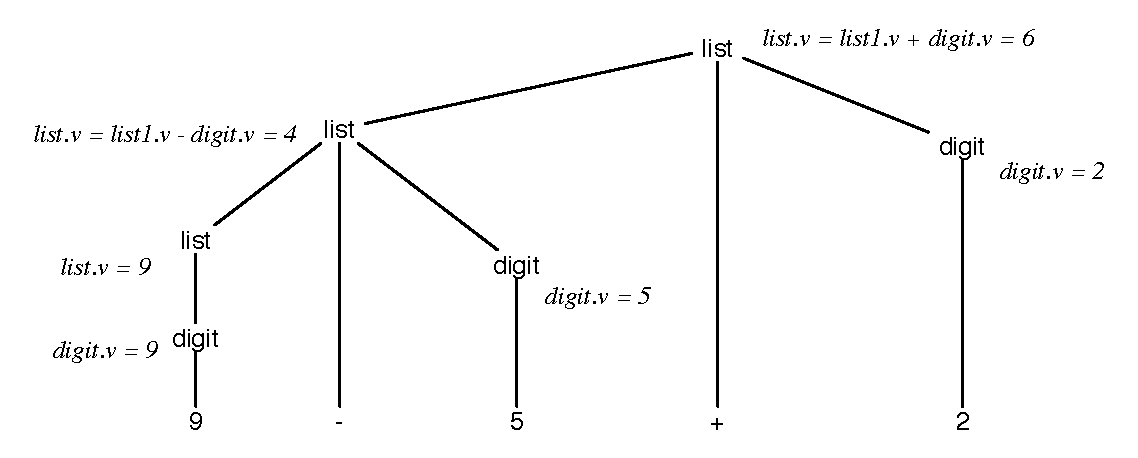
\includegraphics[width=12cm]{figure/parse_tree_appl.pdf}
 \end{center}
 \caption{$B2r@OLZ$K$h$k<0$NCM$N7W;;(B}
 \label{190545_30Mar06}
\end{figure}

\section{$B:G:8F3=P!":G1&F3=P(B}

$BJ8K!(B$G$$B$N3+;O5-9f(B$S$$B$+$iF3=P$5$l$kJ87A<0$K$O!"Hs=*C<5-9f$,J#?t8D4^$^$l$k(B
$B$3$H$,$"$k!#$3$N$&$A!"$I$NHs=*C<5-9f$+$iCV$-49$($r9T$C$F$$$/$+$OG$0U$G$"(B
$B$k!#$I$3$+$iCV$-49$($r9T$C$F$b!":G=*E*$KF@$i$l$kJ8$OEy$7$/!"BP1~$9$k2r@O(B
$BLZ$bEy$7$$!#(B

$BNc$($P!"J8K!(B$E \rightarrow E + E \mid E * E \mid (E) \mid -E \mid {\bf
id}$$B$K$*$$$F!"J8(B$-({\bf id}+{\bf id})$$B$rF3=P$9$kJ}K!$O<!$N$h$&$J$b$N(B
$B$,$"$k!#(B
\[
 E \Rightarrow -E \Rightarrow -(E) \Rightarrow -(E+E) \Rightarrow
  -({\bf id}+E) \Rightarrow -({\bf id}+{\bf id})
\]
\[
 E \Rightarrow -E \Rightarrow -(E) \Rightarrow -(E+E) \Rightarrow
  -(E+{\bf id}) \Rightarrow -({\bf id}+{\bf id})
\]

$B$3$NNc$G$O(B2$BDL$j$@$1$@$,!"0lHL$K$O$b$C$HB?$/$NF3=P$,$"$jF@$k!#$3$l$i$NF3=P(B
$B$NCf$G!"(B``$BI8=`7A(B''$B$H8@$($k$b$N$rDj$a$F$*$/$3$H$K$7$h$&!#I,$:J87A<0$N0lHV(B
$B:8$NHs=*C<5-9f$rCV$-49$($k$h$&$JF3=P$r(B{\bfseries $B:G:8F3=P(B}$B!J(Bleftmost
derivation$B!K!"0lHV1&$NHs=*C<5-9f$rCV$-49$($k$h$&$JF3=P$r(B{\bfseries $B:G1&F3(B
$B=P(B}$B!J(Brightmost derivation$B!K$H$$$&!#>e$NNc$G$O!"(B1$BHVL\$N$b$N$,:G:8F3=P!"(B2$BHV(B
$BL\$N$b$N$,:G1&F3=P$G$"$k!#(B

$B9=J82r@O$G$O!":G:8F3=P$,Hs>o$K=EMW$JLr3d$r2L$?$9(B\footnote{$BK\9V5A$G?($l$J(B
$B$+$C$?>e8~$-9=J82r@O$H$$$&<jK!$G$O!":G1&F3=P$,=EMW$JLr3d$r2L$?$9!#(B}$B!#(B

\section{$B[#Kf$JJ8K!(B}
\label{121131_31Mar06}

1$B$D$NJ8$KBP$7$F(B2$B$D0J>e$N2r@OLZ$,:n$l$kJ8K!$r(B{\bfseries $B[#Kf$G$"(B
$B$k(B}$B!J(Bambiguous$B!K$H$$$&!#9=J82r@O$G$O(B2$B$D0J>e$N2r@OLZ$,$G$-$F$7$^$&$N$O:$$k(B
$B$N$G!"[#Kf$G$J$$J8K!$KJQ49$7$?$j!"$"$k<o$N5,B'$r@_$1$FJ#?t$N2r@OLZ$+$i(B1$B$D(B
$B$rA*$V$h$&$K$7$?$j$9$k!#(B

$B[#Kf$5$r2r>C$9$kJ}K!$O!"$"$^$jBN7OE*$K$O$J$C$F$$$J$$!#LdBj(B
\ref{ex:cfg_03}$B$NJ8K!$O[#Kf$G$"$k$,!"(B\eqref{171007_30Mar06}$B$NJ8K!$KJQ7A$9(B
$B$l$P[#Kf$5$O2r>C$G$-$k!#(B

$B$b$&(B1$B$DNc$r5s$2$h$&!#(B
\begin{align*}
 stmt & \rightarrow  {\bf if}\ (expr)\ stmt\  \\
      & \quad \mid {\bf if}\ (expr)\ stmt\ {\bf else}\ stmt \\
      & \quad \mid S_1 \mid S_2 \mid S_3 \\
 expr & \rightarrow  E_1 \mid E_2
\end{align*}
$B>e$K<($7$?$N$O(Bif$BJ8$rI=$9J8K!$G$"$k!#$7$+$7!"?^(B
\ref{fig:ambiguous_grammar}$B$GJ,$+$k$h$&$K!"$3$NJ8K!$O<!$NJ8$KBP$7$F(B2$B$D$N(B
$B2r@OLZ$r@8@.$9$k$N$G!"[#Kf$G$"$k!#(B
\[
 {\bf if}\ (E_1)\ S_1\ {\bf else}\ {\bf if}\ (E_2)\ S_2\ {\bf else}\ S_3
\]

\begin{figure}[]
 \begin{center}
  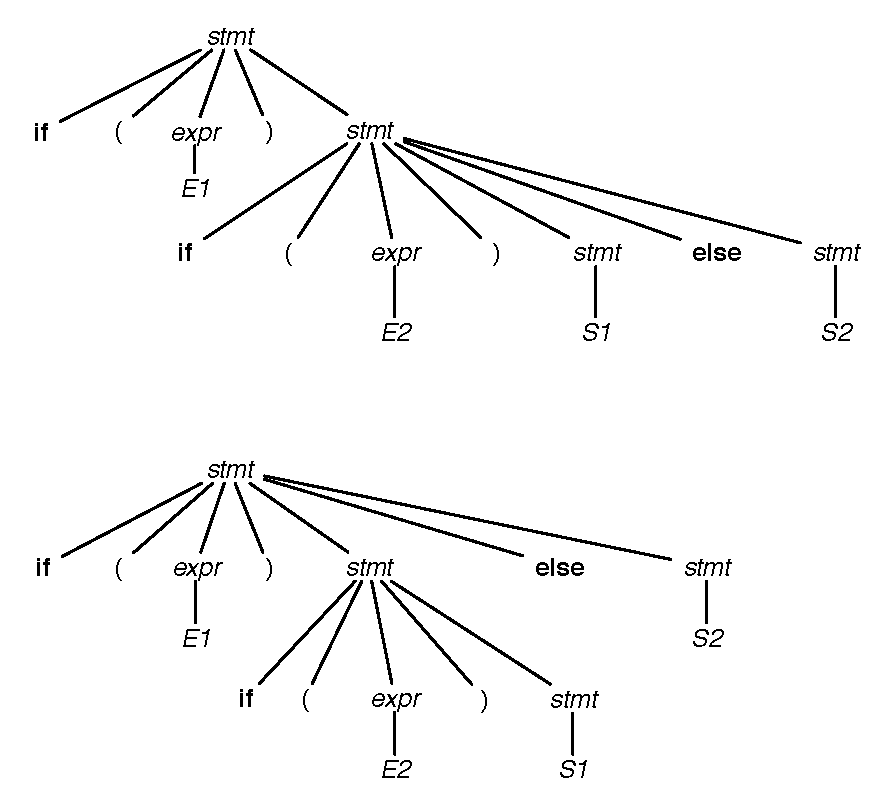
\includegraphics[scale=0.8]{figure/fig46.pdf}
 \end{center}
 \caption{$B[#Kf$JJ8K!$KBP$9$k(B2$B$D$N2r@OLZ(B}
 \label{fig:ambiguous_grammar}
\end{figure}

$B$3$N$h$&$J>r7oJ8$NJ8K!$G$OIaDL!"!V3F(Belse$B$OA0$N$[$&$K$"$kL$BP1~$N(Bthen$BJ8$N(B
$B$&$A!"$b$C$H$b6a$$$b$N$HBP1~$9$k!W$H$$$&5,B'$r@_$1!"[#Kf@-$r2r>C$9$k!#$D(B
$B$^$j?^(B\ref{fig:ambiguous_grammar}$B$N2r@OLZ$N$&$A!">e$N$[$&$r:NMQ$9$k!#<!$N(B
$B$h$&$KJ8K!$r=q$-49$($k$3$H$G!"[#Kf$5$,2r>C$G$-$k!#(B

\begin{align*}
 stmt & \rightarrow matched\_stmt \\
      & \quad\mid        unmatched\_stmt \\
 matched\_stmt & \rightarrow {\bf if}\ (expr)\ matched\_stmt\ {\bf
  else}\ matched\_stmt \\
      & \quad\mid S_1 \mid S_2 \mid S_3 \\
 unmatched\_stmt & \rightarrow {\bf if}\ (expr)\ stmt \\
                 & \quad\mid        {\bf if}\ (expr)\ matched\_stmt\ {\bf
		  else}\ unmatched\_stmt \\
 expr & \rightarrow E_1 \mid E_2
\end{align*}

\section{$B:8:F5"(B}
\label{121145_31Mar06}

$A \stackrel{*}{\Rightarrow} A\alpha$$B$H$$$&F3=P$,B8:_$9$k$H$-!"$3$NJ8K!$O(B
{\bfseries $B:8:F5"(B}$B$G$"$k$H$$$&!#8e=R$9$k$,!":8:F5"$NJ8K!$O9=J82r@O$G$O07(B
$B$$$,$d$C$+$$$G$"$k!#FC$KK\9V5A$G=R$Y$k<jK!$G$O!"9=J82r@O$,Dd;_$7$J$$>u67(B
$B$,5/$3$C$F$7$^$&!#(B

$B9,$$!":8:F5"J8K!$O!"$=$l$HEy2A!JF1$88@8l$r@8@.$9$k!K$G:8:F5"$r4^$^$J$$J8(B
$BK!$KI,$:JQ7A$9$k$3$H$,$G$-$k!#$3$3$G$O!"(B$A \rightarrow A\alpha$$B$H$$$&7A$N(B
$B@8@.5,B'$r;}$D:8:F5"J8K!$r!":8:F5"$G$O$J$$J8K!$KJQ49$9$kJ}K!$N$_<($9!#:8(B
$B:F5"$NJ8K!$N(BA-$B@8@.5,B'$O!"0lHL$K(B
\[
 A \rightarrow A\alpha_1 \mid A\alpha_2 \mid \cdots \mid A\alpha_m \mid \beta_1 \mid
 \beta_2 \mid \cdots \mid \beta_n
\]
$B$H=q$1$k!#$3$3$G(B$\beta_i$$B$O(B$A$$B0J30$N5-9f$G;O$^$k5-9fNs$G$"$k!#$3$N$H$-!"(B
$B$3$N(BA-$B@8@.5,B'$r<!$N$h$&$KJQ7A$9$k!#(B
\begin{eqnarray*}
 A & \rightarrow & \beta_1 A' \mid \beta_2 A' \mid \cdots \mid \beta_n A' \\
 A' & \rightarrow & \alpha_1 A' \mid \alpha_2 A' \mid \cdots \mid \alpha_m A' \mid \epsilon
\end{eqnarray*}
$B$3$NJ8K!$O!"JQ7AA0$N$b$N$HF1$88@8l$r@8@.$7!"$+$D:8:F5"$r4^$^$J$$!#(B

\section{$BJ8L.<+M3J8K!$N8B3&(B}
\label{110128_3Apr06}

$B8@8l(B$L = \{wcw \mid w \in (a \mid b)^* \}$$B$O!V(B$c$$B$NA08e$KF1$8J8;zNs(B$w$$B$,(B
$B=P8=$9$k$h$&$J8@8l!W$G$"$j!"%W%m%0%i%_%s%08@8l$G$N!VJQ?t$r;H$&$H$-$K$O!"(B
$B$=$l$h$jA0$K@k8@$r$7$F$*$+$J$1$l$P$J$i$J$$!W$H$$$&7h$^$j$rCj>]2=$7$?$b$N(B
$B$H8@$($k!#$H$3$m$,!"<B$O(B$L$$B$OJ8L.<+M3J8K!$G$OI=8=$G$-$J$$!#$D$^$j!"JQ?t$r(B
$B;H$&A0$K@k8@$5$l$F$$$k$+8!::$9$k$N$O!"9=J82r@OIt$G$O9T$&$3$H$,$G$-$J$$!#(B
$B<B:]!"$3$N8!::$O!"0UL#2r@OIt$G9T$o$l$F$$$k!#(B

$B$3$N$h$&$K!"%W%m%0%i%_%s%08@8l$N@)8B$K$O9=J82r@OIt$G8!::$G$-$J$$$b$N$,$"(B
$B$j!"$=$l$i$O0UL#2r@OIt$G8!::$5$l$k$3$H$,B?$$!#(B

\section*{$BN}=,LdBj(B}

\begin{exercise}
 \label{ex:cfg_03}
 $B<!$NJ8L.<+M3J8K!$K$D$$$F!"%H!<%/%sNs(B 8 - 2 + 6 $B$N2r@OLZ$r<($;!#2DG=$J$9(B
 $B$Y$F$N>l9g$r<($7!"<+A3$J<0$N0UL#$K$J$k$b$N$O$I$l$+<($;!#(B
 \[
  string \rightarrow string + string \mid string - string \mid 0 \mid 1
 \mid 2 \mid 3 \mid 4 \mid 5 \mid 6 \mid 7 \mid 8 \mid 9
 \]
\end{exercise}
\begin{exercise}
 $BJ8L.<+M3J8K!(B$S \rightarrow 0 S 1 \mid 0 1$$B$O$I$N$h$&$J8@8l$rI=$9$+=R$Y$h!#(B
 \label{ex:cfg_04}
\end{exercise}
\begin{exercise}
 $B<!$NJ8K!$r9M$($k!#(B
  \begin{eqnarray*}
   S & \rightarrow & A1B \\
   A & \rightarrow & 0A \mid \epsilon \\
   B & \rightarrow & 0B \mid 1B \mid \epsilon
  \end{eqnarray*}
 $B$3$NJ8K!$KBP$7!"J8;zNs(B$00101$$B$N:G:8F3=P!":G1&F3=P$r<($;!#(B
 \label{ex:cfg_01}
\end{exercise}
\begin{exercise}
 $B;;=Q<0$KBP$9$kJ8K!(B
  \begin{eqnarray*}
   E & \rightarrow & E + T \mid T \\
   T & \rightarrow & T * F \mid F \\
   F & \rightarrow & (E) \mid {\bf id}
  \end{eqnarray*}
 $B$r!":8:F5"$G$J$$$h$&$KJQ7A$;$h!#(B
 \label{ex:cfg_02}
\end{exercise}

%#!platex main

\newcommand{\First}{{\sf FIRST}}
\newcommand{\Follow}{{\sf FOLLOW}}
\newcommand{\Director}{{\sf DIRECTOR}}

\chapter{$B9=J82r@O(B}

\section{$B9=J82r@O$N<jK!(B}

$B9=J82r@OIt$O!";z6g2r@OIt$+$i=PNO$5$l$?%H!<%/%sNs$rFI$_9~$_!"86;O%W%m%0%i(B
$B%_%s%08@8l$NJ8K!$KE,9g$7$F$$$k$+2r@O$7!"E,9g$7$F$$$k>l9g$O%H!<%/%s$r0UL#(B
$B$N$^$H$^$j$rH?1G$7$?F~$l;R9=B$$K%0%k!<%W2=$7$?$b$N$r=PNO$9$k!#(B

$B$H$3$m$G!"86;O%W%m%0%i%`8@8l$NJ8K!$,!J%H!<%/%s$r=*C<5-9f$H$9$k$h$&$J!KJ8(B
$BL.<+M3J8K!$G5-=R$5$l$F$$$k!"$H$7$h$&!#$9$k$H!"9=J82r@OIt$N=PNO$O!"%H!<%/(B
$B%sNs$r7k2L$H$9$k$h$&$J2r@OLZ$KB>$J$i$J$$!#$D$^$j9=J82r@O$H$O!"J8L.<+M3J8(B
$BK!$r$b$H$K%H!<%/%sNs$rF3=P$7!"2r@OLZ$r9=@.$9$k:n6H$=$N$b$N$G$"$k!#$?$@$7!"(B
$B9M$($F$*$+$J$1$l$P$J$i$J$$$3$H$,$$$/$D$+$"$k!#(B

1$B$DL\$O!"9=J82r@O$N7W;;NL!J7W;;;~4V!K$G$"$k!#$I$s$JJ8L.<+M3J8K!$G$b!"$=$l(B
$B$K4p$E$$$?9=J82r@O%k!<%A%s$O:n$l$k$N$@$,!"0lHL$K$O!"D9$5(B$n$$B$N%H!<%/%sNs$N(B
$B9=J82r@O$K(B$O(n^3)$$B$N;~4V$,I,MW$H$J$C$F$7$^$&$N$G$"$k!#BP>]$H$9$k%H!<%/%s(B
$BNs$,86;O%W%m%0%i%`$G$"$j!"%5%$%:$,Bg$-$/$J$j$&$k$3$H$r9M$($k$H!"$3$l$G$O(B
$B7W;;;~4V$,$+$+$j$9$.$k$H8@$($k!#$=$3$G!"%3%s%Q%$%i$N9=J82r@O$G$O!"J8K!$K(B
$B@)8B$r2C$(!"(B$O(n)$$BDxEY$N;~4V$G9=J82r@O$r2DG=$K$9$k$N$,IaDL$G$"$k!#(B

2$B$DL\$O!"9=J82r@O%W%m%0%i%`$N@_7W$NJ}?K$G$"$k!#BP>]$H$9$k%H!<%/%sNs$ND9$5(B
$B$,;vA0$K$OJ,$+$i$:!"$+$DBg$-$/$J$j$&$k$?$a!"%H!<%/%sNs$r$"$i$+$8$aA4ItFI(B
$B$_9~$s$G$+$i2r@O$r9T$&!"$H$$$&%W%m%0%i%`@_7W$O9%$^$7$/$J$$!#$=$3$G!"$3$N(B
$B9V5A$G$O!";z6g2r@OIt$+$i9=J82r@OIt$K(B1$B%H!<%/%s$:$DEO$7$J$,$i2r@O$r9T$&!"$H(B
$B$$$&<jK!$r$H$k!#$3$N$?$a!"8+$+$1>e!"J8L.<+M3J8K!$G$NF3=P$H$O0[$J$k%"%k%4(B
$B%j%:%`$K$J$C$F$$$k!#(B

$B9=J82r@O$N<jK!$K$O!"2r@OLZ$r:n$kJ}8~$K$h$C$FBg$-$/(B2$B<oN`$KJ,$1$i$l$k!#:,$+(B
$B$iMU$K8~$1$F:n$k<jK!$r(B{\bfseries $B2<8~$-9=J82r@O(B}$B!J(Btop-down parsing$B!K!"MU(B
$B$+$i:,$K8~$1$F:n$k<jK!$r(B{\bfseries $B>e8~$-9=J82r@O(B}$B!J(Bbottom-up parsing$B!K$H(B
$B$$$&!#2<8~$-9=J82r@O$N$[$&$,<jK!$H$7$F$O0W$7$/!"<j:n6H$G9=J82r@O%k!<%A%s(B
$B$r:n$l$k$,!"J8K!$KBP$9$k@)8B$OBg$-$$!#$?$@$7!"$=$l$G$b$[$H$s$I$N%W%m%0%i(B
$B%_%s%08@8l$N9=J82r@O$K$O==J,$G$"$k!#$=$3$G!"$3$N9V5A$G$O!"2<8~$-9=J82r@O(B
$B$K9J$C$F2r@b$9$k!#(B

\section{$BM=B,7?9=J82r@O(B}

$B<!$NJ8L.<+M3J8K!$rNc$K$H$j!"2<8~$-9=J82r@O$r@bL@$7$h$&!#$3$NJ8K!$O(BPascal
$B$H$$$&%W%m%0%i%_%s%08@8l$N7?@k8@$N0lIt$G$"$k!#(B
\begin{equation}
\begin{split}
 type & \rightarrow simple \mid \text{\^{}}\ id
 \mid \text{{\sffamily array}}\ \text{{\sffamily [}}\ simple\ \text{{\sffamily ]}}\ \text{{\sffamily of}}\ type \\
 simple & \rightarrow \text{{\sffamily integer}} \mid \text{{\sffamily
 char}} \mid \text{{\sffamily num}}\ \text{{\sffamily dotdot}}\ \text{{\sffamily num}}
\end{split}\label{151415_10Apr06}
\end{equation}

$B$3$NJ8K!$G%H!<%/%sNs(B\icode{array [ num dotdot num ] of integer}$B$N2r@OLZ$r(B
$B:n$k2aDx$r?^(B\ref{154017_30Mar06}$B$K<($9!#(B

\begin{figure}
 \begin{center}
  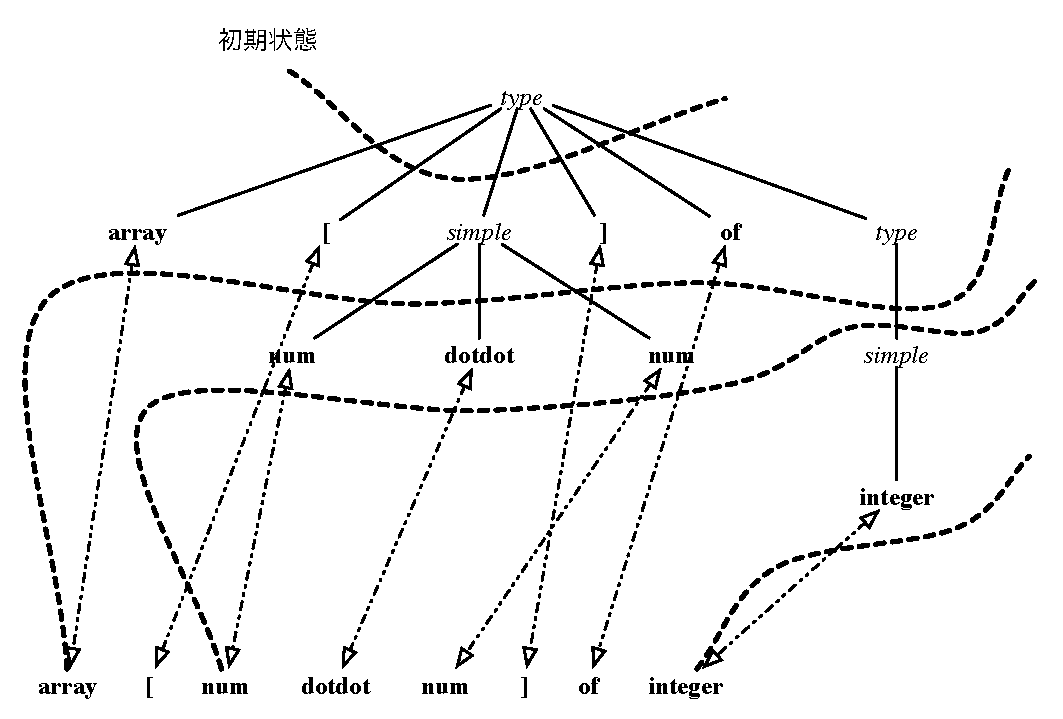
\includegraphics[width=12cm]{figure/making_parse_tree.pdf}
 \end{center}
 \caption{$B2r@OLZ$N9=@.2aDx(B}
 \label{154017_30Mar06}
\end{figure}

$B:G=i!"@aE@$O3+;O5-9f(B$type$$B$@$1$G$"$j!"@)8f$O$3$N@aE@$K$"$k!#;z6g2r@OIt$+(B
$B$i@hF,$N%H!<%/%s(B{\sf array}$B$,EO$5$l$k$H!"(B$type$$B$r:8JU$K;}$D@8@.5,B'$N$&$A!"(B
{\sf array}$B$r@hF,$H$9$k5-9fNs$r@8@.$9$k2DG=@-$N$"$k5,B'$rC5$9!#$3$N>l9g$O(B
$type \rightarrow {\sf array [}\ simple\ {\sf ] of}\ type$$B$N$_$,3:Ev$9$k!#(B
$B$=$3$G!"$3$N5,B'$N1&JU$N3F5-9f$r!"=g$K(B$type$$B$N;R@aE@$H$7!"@)8f$r;R@aE@$N(B
$B@hF,!"$9$J$o$A(B{\sf array}$B$H%i%Y%kIU$1$5$l$?@aE@$K0\$9!#%i%Y%k(B{\sf array}
$B$O=*C<5-9f$J$N$G!"8=:_$N%H!<%/%s(B{\sf array}$B$H>H9g$9$k!#>H9g$K@.8y$9$l$P!"(B
$B<!$N%H!<%/%s$rFI$_9~$_!"$^$?!"8=:_$N2r@OLZ$G?<$5M%@h=g$K<!$N@aE@!"$D$^$j(B
{\sf [}$B$H%i%Y%kIU$1$5$l$?@aE@$K@)8f$r0\$7$F!"F1MM$N=hM}$rB3$1$k!#(B

$B$3$N=hM}$+$iJ,$+$k$h$&$K!">e$NJ8K!$G$O!"%H!<%/%sNs$r:8$+$i1&$K(B1$B2sAv::$9$k(B
$B$@$1$G2<8~$-$K2r@OLZ$r9=@.$9$k$3$H$,$G$-$k!#$3$N$h$&$J!J2<8~$-!K9=J82r@O(B
$B<jK!$rFC$K(B{\bfseries $BM=B,7?9=J82r@O(B}$B!J(Bpredictive parsing$B!K$H$$$&!#!VM=B,!W(B
$B$H$$$&8@MU$O!"<!$K:n$m$&$H$7$F$$$k@a$,Hs=*C<5-9f$N>l9g!"8=:_$N%H!<%/%s(B1$B$D(B
$B$@$1$G!"$I$N@8@.5,B'$rE,MQ$7$FF3=P$r?J$a$l$P$h$$$+!"M=B,$G$-$k$H$$$&;v<B(B
$B$KM3Mh$7$F$$$k!#(B

$B8e=R$9$k$h$&$K!"M=B,7?9=J82r@O%k!<%A%s$OHs>o$K4JC1$K<BAu$G$-$k!#$7$+$7!"(B
$B$I$s$JJ8K!$G$bM=B,7?9=J82r@O$,9T$($k$o$1$G$O$J$$!#$+$J$j@)8B$5$l$?7A$NJ8(B
$BK!$G$7$+!"$3$N2r@O<jK!$O;H$($J$$!#$=$l$G$b!"<BMQ>e$O!"M=B,7?9=J82r@O$,9T(B
$B$($kDxEY$NJ8K!$G=<J,$J>l9g$,$+$J$jB?$$!#(B

$BJ8K!(B$G$$B$K$D$$$FM=B,7?9=J82r@O$,2DG=$G$"$k$?$a$K$O!"(B$G$$B$,<!$N$h$&$J@)8B$r(B
$BK~$?$7$F$$$J$1$l$P$J$i$J$$!#(B
\begin{enumerate}
 \item $G$$B$O[#Kf$G$J$/!"$+$D:8:F5"$G$O$J$$!#(B
 \item $B@8@.5,B'(B$A \rightarrow \alpha_1 \mid \alpha_2 \mid \cdots \mid
       \alpha_n $$B$K$D$$$F!"8=:_$NF~NO5-9f(B$a$$B$N$_$+$i$I$N@8@.5,B'$G(B$A$$B$r=q(B
       $B$-49$($l$P$h$$$+!"0l0U$K7hDj$G$-$J$1$l$P$J$i$J$$!#(B
\end{enumerate}

$B0J2<$GBP>]$H$9$k$N$O!"[#Kf$G$J$/!":8:F5"$G$O$J$$J8K!$H$9$k!#$b$79=J82r@O(B
$B$r9T$$$?$$J8K!$,[#Kf$G$"$C$?$j:8:F5"$G$"$C$?$j$9$k>l9g$O!"(B
\ref{121131_31Mar06}$B@a$d(B\ref{121145_31Mar06}$B@a$N<jK!$rMQ$$$F!"[#Kf$G$J$/(B
$B:8:F5"$G$J$$J8K!$KJQ7A$7$F$*$+$J$1$l$P$J$i$J$$!#(B

\section{LL(1)$BJ8K!(B}
\label{160007_10Apr06}

$BM=B,7?9=J82r@O$N2DG=$JJ8K!$H$7$F!"(B{\bfseries LL(1)$BJ8K!(B}$B!J(BLL(1) grammar$B!K(B
$B$H$$$&J8K!$r>R2p$9$k!#B?$/$N%W%m%0%i%_%s%08@8l$NJ8K!$O(BLL(1)$BJ8K!$K<}$^$C$F(B
$B$$$k$3$H$,CN$i$l$F$$$k!#(B

\subsection{\First $B$H(B\Follow}

$B$^$:(B\First $B$H(B\Follow $B$H$$$&(B2$B$D$N=*C<5-9f=89g$rF3F~$7$F$*$3$&!#(B

$BG$0U$N5-9fNs(B$\alpha$$B$KBP$7!"(B$\alpha$$B$+$iF3=P$5$l$k5-9fNs$NCf$G@hF,$K8=$l(B
$B$k=*C<5-9f$N=89g$r(B$\First(\alpha)$$B$H$$$&!#$?$@$7(B$S
\stackrel{*}{\Rightarrow} \epsilon$$B$N>l9g$O(B$\epsilon$$B$b(B
$\First(\alpha)$$B$K4^$a$k!#(B

$BHs=*C<5-9f(B$A$$B$KBP$7!"J87A<0$NCf$G!"(B$A$$B$N$9$08e$m$K8=$l$k2DG=@-$N$"$k=*C<(B
$B5-9f$N=89g$r(B$\Follow(A)$$B$H$9$k!#(B$A$$B$,J87A<0$N0lHV8e$m$K$J$k$3$H$,(B
$B$"$k>l9g$K$O!"5-9fNs$NKvHx$rI=$9FC<l$J=*C<5-9f(B$\$$$B$r(B$\Follow(A)$
$B$K4^$a$k!#(B

\begin{example}
 \label{ex:first_follow}
 $B<!$N!J[#Kf$G$J$/:8:F5"$G$J$$!KJ8K!$r9M$($k!#(B
 \begin{align*}
  E & \rightarrow TE' \\
  E' & \rightarrow + TE' \mid \epsilon \\
  T & \rightarrow FT' \\
  T' & \rightarrow * FT' \mid \epsilon \\
  F & \rightarrow (E) \mid \mathbf{id}
 \end{align*}
 $B$3$NJ8K!$KBP$7!"(B\First $B$r5a$a$k$H<!$N$h$&$K$J$k!#(B
 \begin{align*}
  & \First(E) = \First(T) = \First(F) = \{(, \mathbf{id}\} \\
  & \First(E') = \{+, \epsilon\} \\
  & \First(T') = \{*, \epsilon\} \\
  & \First(TE') = \First(T) = \{(, {\bf id}\} \\
  & \First(\epsilon) = \{\epsilon\} \\
  & \First(+TE') = \{+\} \\
  & \First(FT') = \First(F) = \{(, {\bf id}\} \\
  & \First(*FT') = \{*\} \\
  & \First((E)) = \{(\} \\
  & \First({\bf id}) = \{{\bf id}\}
 \end{align*}
 $B$^$?(B\Follow $B$r5a$a$k$H<!$N$h$&$K$J$k!#(B
 \begin{align*}
  & \Follow(E) = \Follow(E') = \{), \$\} \\
  & \Follow(T) = \Follow(T') = \{+, ), \$\} \\
  & \Follow(F) = \{+, *, ), \$\}
 \end{align*}
 $\Box$
\end{example}

\subsection{\First $B$N7W;;J}K!(B}

\begin{enumerate}
 \item $B=*C<5-9f(B$a$$B$K$D$$$F(B$\First(a) = \{a\}$
 \item $\epsilon$$B$K$D$$$F(B$\First(\epsilon) = \{\epsilon\}$ 
 \item $B@8@.5,B'(B$X \rightarrow a\alpha$$B$K$D$$$F!"(B$a$$B$r(B$\First(X)$
       $B$K2C$($k!#(B
 \item $B@8@.5,B'(B$X \rightarrow \epsilon$$B$K$D$$$F!"(B$\epsilon$$B$r(B
       $\First(X)$$B$K2C$($k!#(B
 \item $B@8@.5,B'(B$X \rightarrow Y_1Y_2\cdots Y_n$$B$K$D$$$F(B
       \begin{itemize}
	\item $Y_1$$B$,(B$\epsilon$$B$rF3=P$7$J$$$J$i$P(B$\First(Y_1)$$B$r(B
	      $\First(X)$$B$K2C$($k(B
	\item $Y_1 \stackrel{*}{\Rightarrow} \epsilon$$B$G$"$l$P!"(B
	      $\First(Y_1) - \{\epsilon\}$$B$r(B$\First(X)$$B$K2C$($k!#$5$i$K(B
	      $Y_2$$B$,(B$\epsilon$$B$rF3=P$7$J$$$J$i$P!"(B$\First(Y_2)$$B$r(B
	      $\First(X)$$B$K2C$(!"(B$Y_2 \stackrel{*}{\Rightarrow}
	      \epsilon$$B$J$i$P(B$\First(Y_2) - \{\epsilon\}$$B$r(B
	      $\First(X)$$B$K2C$($k!#(B($B0J2<F1MM(B)
	\item $Y_1Y_2\cdots Y_n \stackrel{*}{\Rightarrow} \epsilon$$B$J$i$P!"(B
	      $\epsilon$$B$r(B$\First(X)$$B$K2C$($k(B
	      \label{170823_7Jun05}
       \end{itemize}
 \item $\First(X_1X_2\cdots X_n)$$B$O(B\ref{170823_7Jun05}$B$HF1MM$K7W;;(B
\end{enumerate}

$B5,B'(B\ref{170823_7Jun05}$B$,$d$dJ,$+$j$K$/$$$+$b$7$l$J$$!#Nc$($P!"@8@.5,B'(B$X \rightarrow
Y_1Y_2$$B$K$D$$$F!"$"$k=*C<5-9f(B$x$$B$,(B$\First(X)$$B$K4^$^$l$k$N$O!"<!$N$$$:$l(B
$B$+$N>l9g$K8B$i$l$k!#(B
\begin{enumerate}
 \item $x \in \First(Y_1)$
 \item $Y_1 \stackrel{*}{\Rightarrow} \epsilon$$B$+$D(B$x \in \First(Y_2)$
\end{enumerate}
$B$D$^$j(B$Y_1$$B$+$i=*C<5-9f$,2?$b@8@.$5$l$J$$2DG=@-$,$"$k$J$i$P!"(B
$\First(Y_2)$$B$NMWAG$b(B$\First(X)$$B$K4^$^$l$k!"$H$$$&$3$H$G$"$k!#5,B'(B
\ref{170823_7Jun05}$B$O$3$l$r0lHLE*$K$7$?$b$N$G$"$k!#(B

\subsection{\Follow $B$N7W;;J}K!(B}

\begin{enumerate}
 \item $\Follow(S)$$B$K(B$\$$$B$r2C$($k!#(B
 \item $B$I$N(B\Follow $B$K$b5-9f$,DI2C$5$l$J$/$J$k$^$G!"0J2<$r7+$jJV$9!#(B
       \begin{itemize}
	\item $A \rightarrow \alpha B\beta$$B$K$D$$$F!"(B$\First(\beta)
	      - \{\epsilon\}$$B$r(B$\Follow(B)$$B$K2C$($k!#(B
	\item $A \rightarrow \alpha B\beta$$B!"$+$D(B$\First(\beta)$
	      $B$,(B$\epsilon$$B$r4^$s$G$$$k$H$-!"(B$\Follow(A)$$B$r(B
	      $\Follow(B)$$B$K2C$($k!#(B
	\item $A \rightarrow \alpha B$$B$N$H$-!"(B$\Follow(A)$$B$r(B
	      $\Follow(B)$$B$K2C$($k!#(B
       \end{itemize}
\end{enumerate}

$B$d$dJ,$+$j$K$/$$%"%k%4%j%:%`$J$N$G!">/$7@0M}$7$F$_$h$&!#(B
$\Follow()$$B$NCM$,JQ2=$9$k$N$O!"<!$N(B3$BDL$j$N>l9g$7$+$J$$!#(B
\begin{itemize}
 \item $B3+;O5-9f(B$S$$B$K$D$$$F!"L5>r7o$K(B$\$$$B$,2C$($i$l$k!#(B
 \item $A \rightarrow \alpha B \beta$$B$N7A$N5,B'$K$D$$$F!"(B$\First(\beta)$
       $B$,(B$\Follow(B)$$B$K2C$($i$l$k!#!J(B$\beta$$B$+$iF3=P$5$l$k5-9fNs$N@hF,$N(B
       $BJ8;z$O(B$B$$B$ND>8e$K8=$l$k$+$i!K(B
 \item $A \rightarrow \alpha B$$B!"$b$7$/$O(B$A \rightarrow \alpha B \beta$
       $B$G(B$\beta$$B$+$i(B$\epsilon$$B$,F3=P$5$l$k!J(B$\beta$$B$,>C$($F$7$^$&!K>l9g(B
       $B$K$D$$$F!"(B$\Follow(A)$$B$,(B$\Follow(B)$$B$K2C$($i$l$k!#!J(B$A$$B$ND>8e$K8=$l(B
       $B$kJ8;z$O(B$B$$B$ND>8e$K$b8=$l$k$+$i!K(B
\end{itemize}
$B$=$3$G!"@8@.5,B'$r8+$J$,$i!"CM$,EAHB$7$F$$$/MM;R$rM-8~%0%i%U$K$7$F$_$k!#(B
$BNc$($P(B$E \rightarrow TE'$$B$+$i(B$\First(E') - \{\epsilon\}$$B$,(B$\Follow(T)$
$B$KEAHB$9$k$3$H$,J,$+$k$N$G!"(B$\First(E')$$B$+$i(B$\Follow(T)$$B$XM-8~;^$r2C$($k!#(B
$B$3$N$H$-!"(B$\First(E')$$B$+$i(B$\{\epsilon\}$$B$r0z$+$J$1$l$P$J$i$J$$$N$G!";^$r(B
$BGK@~$K$7$F$*$/!#$^$?(B$E' \rightarrow +TE' \mid \epsilon$$B$h$j(B$E'
\Rightarrow \epsilon$$B$G$"$k$N$G!"(B$\Follow(E')$$B$,(B$\Follow(T)$$B$KEAHB$9$k$3(B
$B$H$,J,$+$k!#$=$3$G!"(B$\Follow(E')$$B$+$i(B$\Follow(T)$$B$XM-8~;^$r2C$($k!#(B

$B$3$N$h$&$K$9$Y$F$NCM$NEAHB$KBP$7$FM-8~;^$r2C$($k$H!"?^(B
\ref{134551_20Jul07}$B$N$h$&$J%0%i%U$,F@$i$l$k!#$3$N%0%i%U$rMQ$$$F(B
$\Follow$$B$r7W;;$9$k$3$H$,$G$-$k!#$D$^$j!"M-8~;^(B$X \rightarrow Y$$B$,$"$k>l(B
$B9g$O(B$X$$B$NMWAG$r$9$Y$F(B$Y$$B$K2C$($k!#$^$?(B$X $B!D(B> Y$$B$,$"$k>l9g$O(B$X$$B$NMWAG$N$&(B
$B$A(B$\epsilon$$B0J30$r$9$Y$F(B$Y$$B$K2C$($k!#?^(B\ref{134551_20Jul07}$B$r4p$K(B
$\Follow$$B$r7W;;$9$k$H!"Nc(B\ref{ex:first_follow}$B$K<($7$?DL$j$K$J$k$3$H$r3N(B
$B$+$a$h!#(B
\begin{figure}
 \begin{center}
  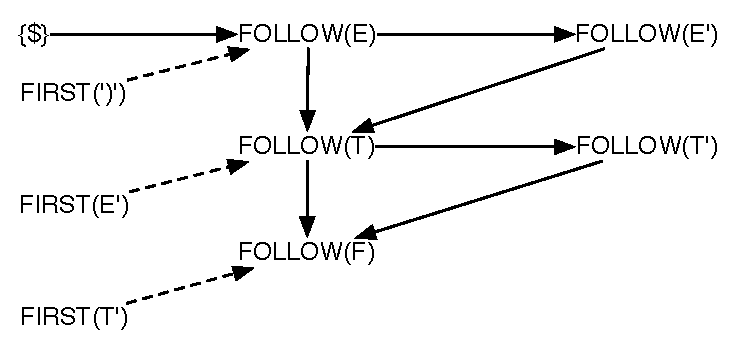
\includegraphics[scale=0.7]{figure/2008040801.pdf}
 \end{center}
 \caption{$\Follow$$B$NCM$NEAHB$rI=$9%0%i%U(B}
 \label{134551_20Jul07}
\end{figure}

\subsection{LL(1)$BJ8K!(B}

\subsubsection{\Director}

$B>e$G=R$Y$?(B\First $B$H(B\Follow $B$rMQ$$$F!"(B\Director $B$H$$$&=*C<5-9f=89g$rDj5A$9(B
$B$k!#@8@.5,B'(B$A \rightarrow \alpha$$B$KBP$7$F(B$\Director(A, \alpha)$$B$O<!$N$h(B
$B$&$J=89g$G$"$k!#(B
\[
 \Director(A, \alpha) = \begin{cases}
			 \First(\alpha) & 
			 \text{$\alpha\stackrel{*}{\Rightarrow}
			 \epsilon$ $B$G$J$$$H$-(B} \\
			 \First(\alpha) \cup \Follow(A) & 
			 \text{$\alpha \stackrel{*}{\Rightarrow} \epsilon$$B$N$H$-(B}
			\end{cases}
\]
$BD>4QE*$K$O!"(B$\Director(A, \alpha)$$B$H$O!"@8@.5,B'(B$A \rightarrow \alpha$$B$r(B
$BE,MQ$7$?$H$-$KF~NO%H!<%/%sNs$N@hF,$K8=$l$k2DG=@-$N$"$k=*C<5-9f$N=89g$G$"$k!#(B
$BIaDL$O(B$\First(\alpha)$$B$K0lCW$9$k$N$@$,!"(B$A$$B$+$i(B$\epsilon$$B$,F3=P$5$l$k2DG=(B
$B@-$N$"$k>l9g$K8B$j!"(B$A$$B$N<!$K=P$F$/$k2DG=@-$N$"$k=*C<5-9f!"$9$J$o$A(B
$\Follow(A)$$B$,2C$($i$l$k!#(B

\begin{example}
 $BNc(B\ref{ex:first_follow}$B$NJ8K!$KBP$7$F(B
 \begin{align*}
  & \Director(E, TE') = \First(T) = \{(, {\bf id}\} \\
  & \Director(E', +TE') = \First(+TE) = \{+\} \\
  & \Director(E', \epsilon) = \Follow(E') = \{), \$\} \\
  & \Director(T, FT') = \First(F) = \{(, {\bf id}\} \\
  & \Director(T', *FT') = \First(*FT') = \{*\} \\
  & \Director(T', \epsilon) = \Follow(T') = \{+, ), \$\} \\
  & \Director(F, (E)) = \First((E)) = \{(\} \\
  & \Director(F, {\bf id}) = \First({\bf id}) = \{{\bf id}\}
 \end{align*}$\Box$
\end{example}

\subsubsection{LL(1)$BJ8K!(B}

$BJ8K!(B$G$$B$N@8@.5,B'$N$&$A!"(B$A \rightarrow \alpha \mid \beta$$B$N7A$N$b$N$K$D(B
$B$$$F>o$K(B
\begin{equation}
 \Director(A, \alpha) \cap \Director(A, \beta) = \emptyset\label{173231_31Mar06}
\end{equation}
$B$G$"$k$H$-!"(B$G$$B$r(B\textbf{LL(1)$BJ8K!(B}$B$H$$$&!#M?$($i$l$?J8L.<+M3J8K!$,(BLL(1)
$BJ8K!$G$"$l$P!"M=B,7?9=J82r@O%W%m%0%i%`$,I,$::n$l$k!#(B

% \begin{enumerate}
%  \item $\alpha$$B$H(B$\beta$$B$OF1$8=*C<5-9f$G;O$^$k5-9fNs$rF3=P$9$k$3$H$,$J$$!#(B
%        \[
%        (\First(\alpha) - \{\epsilon\}) \cap
%        (\First(\beta) - \{\epsilon\}) = \emptyset
%        \]
%  \item $\alpha$$B$H(B$\beta$$B$N$&$A!"(B$\epsilon$$B$rF3=P$9$k$N$O$?$+$@$+0lJ}$@$1(B
%        $B$G$"$k!#(B
%  \item $\beta \stackrel{*}{\Rightarrow} \epsilon$$B$N$H$-!"(B$\alpha$$B$+$i(B
%        $B$O(B$\Follow(A)$$B$K4^$^$l$k=*C<5-9f$G;O$^$k5-9fNs$OF3=P$5$l$J(B
%        $B$$!#$D$^$j(B
%        \[
% 	\beta \stackrel{*}{\Rightarrow} \epsilon $B$N$H$-(B 
%        \First(\alpha) \cap \Follow(A) = \emptyset
%        \]
%        $\alpha \stackrel{*}{\Rightarrow} \epsilon$$B$N$H$-$bF1MM!#(B
% \end{enumerate}

\begin{example}
 $BNc(B\ref{ex:first_follow}$B$NJ8K!$G$O(B
 \begin{align*}
  & \Director(E', +TE') \cap \Director(E', \epsilon) = \emptyset \\
  & \Director(T', *FT') \cap \Director(T', \epsilon) = \emptyset \\
  & \Director(F, (E)) \cap \Director(F, {\bf id}) = \emptyset
 \end{align*}
 $B$7$?$,$C$F!"$3$NJ8K!$O(BLL(1)$BJ8K!$G$"$k!#(B$\Box$
\end{example}

\section{$BM=B,7?9=J82r@O%k!<%A%s$N@_7W(B}

$BM=B,7?9=J82r@O$O!"2r@OLZ$r9=@.$7$D$D?<$5M%@h$K$?$I$k$3$H$r;W$$=P$=$&!#$7(B
$B$?$,$C$F!"M=B,7?9=J82r@O$N%W%m%0%i%`$O!"3FHs=*C<5-9f$KBP$7$F(B1$B$D$N4X?t$rMQ(B
$B0U$7!"@8@.5,B'$N1&JU$K$J$i$C$FBP1~$9$k4X?t8F$S=P$7$r9T$($P$h$$!#F1$8:8JU(B
$A$$B$r;}$D@8@.5,B'$,J#?t$"$k>l9g$O!"(B\Director $B$K4p$E$$$F>l9gJ,$1$r9T$&!#(B

$BJ8K!(B\eqref{151415_10Apr06}$B$KBP$9$k9=J82r@O%k!<%A%s$N<BAuNc$r0J2<$K<($9!#(B
\icode{lookahead}$B$O8=:_Av::Cf$N%H!<%/%s$rJ];}$9$kJQ?t!"(B
\icode{nexttoken()}$B$O<!$N%H!<%/%s$r<hF@$9$k4X?t$G$"$k!#$^$?!"3F%H!<%/%s$O(B
\icode{token}$B7?$NCM$G$"$k$H$9$k(B\footnote{$B<B:]$K(BC$B8@8l$G9=J82r@OIt$r@_7W$9(B
$B$k>l9g$O!"3F%H!<%/%s$r@0?t$GI=$7!"(B\icode{\#define}$B$GJLL>$rIU$1$k$3$H$,B?(B
$B$$!#(B}$B!#(B

$B3F4X?t$O@8@.5,B'$H@53N$KBP1~$7$F$*$j!"BN7OE*$K<BAu$9$k$3$H$,2DG=$G$"$k!#(B

\begin{quote}
\lstinputlisting{code/llparse_example.c}
\end{quote}

\section{LL(1)$BJ8K!$HM=B,7?9=J82r@O$N4XO"(B}

$BJ8K!(B$G$$B$,M=B,7?9=J82r@O2DG=$G$"$k>r7o$r;W$$=P$=$&!#(B
\begin{enumerate}
 \item $G$$B$O[#Kf$G$J$/!"$+$D:8:F5"$G$O$J$$!#(B
 \item $B@8@.5,B'(B$A \rightarrow \alpha_1 \mid \alpha_2 \mid \cdots \mid
       \alpha_n $$B$K$D$$$F!"8=:_$NF~NO5-9f(B$a$$B$N$_$+$i$I$N@8@.5,B'$G(B$A$$B$r=q(B
       $B$-49$($l$P$h$$$+!"0l0U$K7hDj$G$-$J$1$l$P$J$i$J$$!#(B
       \label{172929_31Mar06}
\end{enumerate}
$B$3$l$i$,K~$?$5$l$J$$$H$-!"$J$<M=B,7?9=J82r@O$,$G$-$J$$$N$+9M$($F$_$k!#(B

\subsection{$B[#Kf$5(B}

$B[#Kf$JJ8K!$KBP$7$FM=B,7?9=J82r@O$,$&$^$/$$$+$J$$$N$OL@$i$+$G$"$m$&!#!V[#(B
$BKf$G$"$k!W$H$$$&$3$H$O!"$"$k%H!<%/%sNs$r9M$($k$H!"2r@OLZ$N2DG=@-$,(B2$B$D0J>e(B
$B$"$k$H$$$&$3$H$G$"$k!#$I$A$i$,A*Br$5$l$k$+$O1?<!Bh$G$"$k(B\footnote{$B>pJs?t(B
$B3X$NMQ8l$G8@$&$J$i(B{\bfseries $BHs7hDjE*(B}$B!J(Bnondeterministic$B!K$G$"$k!#(B}$B!#$D$^(B
$B$j!"F1$8%W%m%0%i%`$J$N$K!"%3%s%Q%$%k$9$k$?$S$KF0:n$,JQ$o$C$F$7$^$&$H$$$&(B
$B$3$H$G$"$k!#$3$l$G$O;H$$J*$K$J$i$J$$!#$3$l$O(B\ref{121131_31Mar06}$B@a$G=R$Y(B
$B$?$h$&$KJ8K!$rJQ7A$7$?$j!"5,B'4V$KM%@hEY$r@_$1$k$3$H$G2r7h$G$-$k$3$H$,(B
$B$"$k!#(B

\begin{example}
 C$B8@8l$N(Bif$BJ8$r0lHL2=$7$?<!$NJ8K!$r9M$($k!#(B
 \begin{eqnarray*}
  S & \rightarrow & iES \mid iESeS \mid a \\
  E & \rightarrow & b
 \end{eqnarray*}
 $B$3$l$KBP$7:8C<$N3g$j=P$7$r9T$&$H!"<!$N$h$&$JJ8K!$,F@$i$l$k!#(B
 \begin{eqnarray*}
  S & \rightarrow & iESS' \mid a \\
  S' & \rightarrow & eS \mid \epsilon \\
  E & \rightarrow & b
 \end{eqnarray*}
 $B$3$l$G$b$^$@(BLL(1)$BJ8K!$G$O$J$$!#<B$O$3$NJ8K!$O!"$I$&JQ7A$7$F$b(BLL(1)$B$K$O(B
 $B$J$i$J$$$3$H$,$o$+$C$F$$$k!#$7$+$7!"(B$S' \rightarrow eS$$B$r(B$S'
 \rightarrow \epsilon$$B$h$jM%@h$7$FE,MQ$9$k$3$H$K$9$l$P!"M=B,7?9=J82r@O$,(B
 $B9T$($k!#(B$S'$$B$KBP1~$9$k4X?t$O<!$N$h$&$K$J$k!#(B
 \begin{quote}
  \verb|void S_dash() { match(e); S(); }|
 \end{quote}$\Box$
\end{example}
$B>e$G<($7$?M%@hEY$O!"(B\ref{121131_31Mar06}$B@a$G=R$Y$?5,B'!V3F(B else $B$OA0$N$[(B
$B$&$K$"$kL$BP1~$N(Bthen $BJ8$N$&$A!"$b$C$H$b6a$$$b$N$HBP1~$9$k!W$HF1$8F/$-$r$7(B
$B$F$$$k!#(B

\subsection{$B:8:F5"(B}

$B:8:F5"$G$"$kJ8K!$GM=B,7?9=J82r@O%k!<%A%s$r=q$/$H!":F5"8F$S=P$7$,L58B$KH/(B
$B@8$7$F$7$^$&!#Nc$($P<!$N@8@.5,B'$r9M$($k!#(B
\begin{align*}
 expr & \rightarrow expr\ +\ term \\
 term & \rightarrow 0 \mid 1 \mid 2 \mid 3 \mid 4 \mid 5 \mid 6 \mid 7
 \mid 8 \mid 9
\end{align*}
$B$3$l$KBP1~$9$kM=B,7?9=J82r@O%k!<%A%s$r=q$/$H!"4X?t(B expr() $B$O<!$N$h$&$J(B
$B:F5"4X?t$K$J$k!J@aE@$N@8@.Ey$N%3!<%I$O>J$$$F$$$k!#$^$?7?$bL5;k$7$F$$$k!K!#(B
\begin{quote}
 \verb|expr() { expr(); match(PLUS); term(); }|
\end{quote}
$B$3$l$O:F5"4X?t$G$"$k$,!"4pDl$,B8:_$;$:!"$7$+$b4X?t(B{\sffamily expr()}$B$NFb(B
$BIt$GD>$A$K:F5"8F$S=P$7$,5/$3$C$F$$$k!#$3$l$G$OL@$i$+$KDd;_$7$J$$!#(B

\subsection{\Director $B$N>r7o(B}

$B>r7o(B\ref{172929_31Mar06}$B$O!"(BLL(1)$BJ8K!$G$"$k$?$a$N>r7o(B
\eqref{173231_31Mar06}$B$KB>$J$i$J$$!#$3$N>r7o$rK~$?$5$J$$J8K!$KBP$7$FM=B,(B
$B7?9=J82r@O$r9T$&$H!"2r@O$K<:GT$7$?$H$-$K5-9fNs$r$$$/$i$+La$7!"=hM}$r$d$j(B
$BD>$5$J$1$l$P$J$i$J$$$3$H$,$"$k!#8eLa$j$O0lHL$K=hM}%3%9%H$,9b$/!"$J$k$Y$/(B
$BHr$1$k$N$,K>$^$7$$!#(B

\begin{example}
 $BJ8K!(B$S \rightarrow aBd, B\rightarrow b \mid bc$$B$OL@$i$+$K(BLL(1)$BJ8K!$G$O$J(B
 $B$$!J(B$\Director(B, b)$$B$H(B$\Director(B, bc)$$B$r5a$a$h!K!#$3$NJ8K!$KBP$9$kM=(B
 $BB,7?9=J82r@O%k!<%A%s$r:n$k$H!"<!$N$h$&$K$J$k!#(B
 \begin{quote}
  \verb|void S() { match(a); B(); match(d); }| \\
  \verb|void B() { match(b); $B$^$?$O(B { match(b); match(c); } }|
 \end{quote}
 $B!V$^$?$O!W$H=q$$$?ItJ,$O!V(B\textsf{match(b)}$B$,<:GT$7$?$i(B
 \textsf{match(b); match(c);}$B!W$H$$$&0UL#$G$"$k(B\footnote{$BDL>o$O$3$N$h$&$J(B
 $B8eLa$j$r4^$`%W%m%0%i%`$O:n$i$J$$$?$a!"J,$+$j$d$9$5$r=E;k$7$F!"$"$($FF|K\(B
 $B8l$G<($7$?!#(B}$B!#(B

 $B$3$NJ8K!$K$h$j5-9fNs(B$abcd$$B$r9=J82r@O$9$k2aDx$O<!$N$h$&$K$J$k!#(B
 \begin{enumerate}
  \item \textsf{S()}$B$r8F$S=P$9!#(B
  \item \textsf{S()}$B$NCf$+$i(B\textsf{B()}$B$r8F$S=P$9!#(B
  \item \textsf{B()}$B$NCf$+$i(B\textsf{match(b)}$B$r8F$S=P$9!#$3$N7k2L!"J8(B$abd$
	$B$,F@$i$l$k$,!"$3$l$O(B$abcd$$B$H0lCW$7$J$$$?$a!"9=J82r@O$O<:GT$G$"$j!"(B
	$BF~NO5-9f(B$b$$B$rFI$`A0$N>uBV$K8eLa$j$7!"(B\textsf{B()}$B$KLa$k!#(B
  \item \textsf{B()}$B$NCf$+$i(B\textsf{match(b); match(c);}$B$r8F$S=P$9!#$3$N(B
	$B7k2L!"J8(B$abcd$$B$,F@$i$l!"9=J82r@O$O@.8y$9$k!#(B
 \end{enumerate}

 $B$3$NJ8K!$G$O!":8C<$N3g$j=P$7$r9T$&$3$H$G8eLa$j$,2sHr$G$-$k!#$D$^$jJ8K!$r(B
 $S \rightarrow aBd, B \rightarrow b(c\mid\epsilon)$$B$H=q$-D>$9!#$9$k$H9=J82r(B
 $B@O%W%m%0%i%`$O<!$N$h$&$K$J$j!"8eLa$j$,H/@8$7$J$$!#(B
 \begin{quote}
  \verb|void S() { match(a); B(); match(d); }| \\
  \verb|void B() { match(b); { if (lookahead == 'c') match(c); } }|
 \end{quote}
\end{example}

$B8eLa$j$N5/$3$j$&$kJ8K!$O!":8C<$N3g$j=P$70J30$K!"(BLR(1)$B9=J82r@O$J$I$N>e8~$-(B
$B9=J82r@OK!$K$h$C$F$b9=J82r@O$G$-$k$3$H$,$"$k!#K\9V5A$G$O>\:Y$O>JN,$9$k!#(B

\section*{$BN}=,LdBj(B}

\begin{exercise}\label{exercise20080408}
$B<!$NJ8L.<+M3J8K!Cf$N3FHs=*C<5-9f$K$D$$$F(B{\sffamily FIRST}$B$H(B{\sffamily
 FOLLOW}$B$r7W;;$;$h!#(B
\begin{eqnarray*}
 S & \rightarrow & D \\
 A & \rightarrow & aA \, |\, \epsilon \\
 B & \rightarrow & bAC \, |\, AcD \\
 C & \rightarrow & bC \, | \, Ac \\
 D & \rightarrow & BA \, | \, d
\end{eqnarray*}
\end{exercise}

\begin{exercise}
 $BLdBj(B\ref{exercise20080408}$B$NJ8K!$O(BLL(1)$BJ8K!$+!#(B
\end{exercise}

\begin{exercise}
 $B<!$NJ8K!$,(BLL(1)$BJ8K!$G$"$k$3$H$r<($;!#(B
 \begin{eqnarray*}
  S & \rightarrow & AaAb \mid BbBa \\
  A & \rightarrow & \epsilon \\
  B & \rightarrow & \epsilon
 \end{eqnarray*}
\end{exercise}


%#!platex main

\chapter{$B0UL#2r@O(B}

$B%W%m%0%i%_%s%08@8l$N9=J8>e$N@)Ls$K$O!"J8L.<+M3J8K!$NOH$+$i30$l$k$b$N$,$$(B
$B$/$D$+$"$k!#$3$3$^$G$K$b$H$3$m$I$3$m$G=R$Y$F$-$?$,!"@0M}$7$F$_$h$&!#(B
\begin{itemize}
 \item $BJQ?t$N@k8@$O!"$=$NJQ?t$r;HMQ$9$k$h$j@h$K=P8=$7$J$/$F$O$J$i$J$$!#(B
       \ref{110128_3Apr06}$B@a$G$b=R$Y$?DL$j!"$3$l$OJ8L.<+M3J8K!$G$OI=8=$G(B
       $B$-$J$$!#$b$A$m$s(BLL(1)$BJ8K!$G$bI=8=$G$-$J$$!#(B
       \label{132708_10Apr06}
 \item $B7?$N@09g@-!#Nc$($P(BC$B8@8l$N(B\icode{int x = 10.0 + 2;}$B$H$$$&J8$O!"(B
       \icode{int x = (int)(10.0 + (float)2);}$B!"$D$^$j!"(B(1)$B1&JU$N(B2$B$,(B
       float$B7?$KJQ49$5$l(B (2) 10.0 + 2.0 $B$r7W;;$7!J7k2L$O(B float $B7?!K(B(3)
       int$B7?$KJQ49$5$l$FJQ?t(B x $B$KBeF~$5$l$k!"$H$$$&$h$&$K7W;;$5$l$k!#$3$l(B
       $B$i$N7?JQ49$O!"(BC$B8@8l$NJ8K!$G$OI=8=$5$l$F$*$i$:!";z6g2r@OIt$d9=J82r(B
       $B@OIt$G$O07$($J$$!#(B
\end{itemize}

$B$3$N$h$&$K!"J8L.<+M3J8K!$+$i30$l$k@)Ls$N8!::$d2r@O$O!"9=J82r@OIt$N8e$G9T(B
$B$o$l$k!#$3$l$r(B{\bf $B0UL#2r@O(B}$B!J(Bsemantic analysis$B!K$H$$$&!#0UL#2r@O$O!"9=J8(B
$B2r@O$N=PNO$G$"$k2r@OLZ$rF~NO$H$7!"$=$N2r@OLZ$rJQ7A$7$?$j!"JL$N%G!<%?9=B$(B
$B$r:n@.$7$?$j$9$k!#K\>O$G$O!"0UL#2r@O$N4pAC$H$J$k5;=Q$G$"$kK]Lu%9%-!<%`$K(B
$B$D$$$F=R$Y!"$$$/$D$+$N@)Ls$N8!::$K$D$$$F<BNc$K$h$j@bL@$9$k!#(B

\section{$B5-9fI=(B}

$B86;O%W%m%0%i%`Cf$G$J$s$i$+$NL>A0$,$D$$$F$$$k9=@.MWAG!JJQ?tL>!"4X?tL>!"9=(B
$BB$BN!"9=B$BN$N%a%s%P$J$I!K$rFCD'$E$1$k>pJs$K$O<!$N$h$&$J$b$N$,$"$k!#(B
\begin{itemize}
 \item $B9=@.MWAG$N<oN`!JJQ?t!"4X?t$J$I!K(B
 \item $B9=@.MWAG$NL>A0(B
 \item $B7?>pJs!JJQ?t$N7?!"4X?t$N0z?t$N8D?t!"8D!9$N0z?t$N7?!"JV$jCM$N7?$J(B
       $B$I!K(B
 \item $BB0@-!J(B\icode{static}$B$J$I!K(B
 \item $B9=@.MWAG$,3d$jEv$F$i$l$F$$$kHVCO(B
\end{itemize}
$B$3$l$i$N>pJs$O%3%s%Q%$%i$N3FCJ3,$GIQHK$K;2>H$5$l$k$N$G!"2?$i$+$N7A$N%G!<(B
$B%?9=B$$GI=8=$7!"%3%s%Q%$%iCf$GJ];}!&4IM}$7$J$1$l$P$J$i$J$$!#%3%s%Q%$%i$G(B
$B$ODL>o!"$3$l$i$N>pJs$r(B{\bfseries $B5-9fI=(B}$B!J(Bsymbol table$B!K$H$$$&I=$G4IM}$9$k!#(B

\subsection{$B5-9fI=$N<BAu(B}

$B5-9fI=$r<BAu$9$k:G$b4JC1$JJ}K!$O!"9=B$BN$NG[Ns$rMQ$$$k$b$N$G$"$k!#4JC1$N(B
$B$?$a!"5-9fI=$K3JG<$5$l$k>pJs$r!"<1JL;R$NJ8;zNs!J(B\icode{lexname}$B!":GBgD9$5(B
\icode{MAXLEN}$B!K!"<1JL;R$N%H!<%/%s$N<oN`!J(B\icode{lextoken}$B!K$N(B2$B$D$G$"$k$H(B
$B$7!"5-9fI=$KEPO?$G$-$k%(%s%H%j$N:GBg?t$r(B\icode{MAXENT}$B$H$7$F$*$3$&!#$9$k(B
$B$H!"5-9fI=$rI=$9%G!<%?9=B$$O<!$N$h$&$K$J$k!#(B

\begin{lstlisting}
typedef struct table_ent {
  char lexname[MAXLEN];
  int lextoken;
};
table_ent lextable[MAXENT];
\end{lstlisting}

$B5-9fI=$KBP$9$k<g$JA`:n$O<!$N(B2$B$D$G$"$k!#(B
\begin{itemize}
 \item \icode{int insert(char *s, int t)}$B!DJ8;zNs(B$s$, $B%H!<%/%s(B$t$$B$N%(%s%H(B
       $B%j$r?7$?$K5-9fI=$KEPO?$7!"$=$N%(%s%H%j$NHV9f!JE:;z!K$rJV$9!#$9$G$K(B
       $BEPO?$5$l$F$$$l$P!JEPO?$G$-$J$$$H$7$F!K(B-1 $B$rJV$9!#(B
 \item \icode{int lookup(char *s)}$B!DJ8;zNs(B$s$$B$N%(%s%H%j$,5-9fI=$KEPO?$5$l(B
       $B$F$$$k$+D4$Y$k!#$"$l$P$=$N%(%s%H%j$NHV9f!JE:;z!K$rJV$7!"$J$1$l$P(B
       -1 $B$rJV$9!#(B
\end{itemize}

$B>e5-$N9=B$BN$NG[Ns$K$h$k5-9fI=$KBP$7!"$3$l$i$NA`:n$r(BC$B8@8l$G<BAu$9$k$3$H$O(B
$BMF0W$G$"$m$&!#3F<+$G;n$_$i$l$?$$!#(B

$B<B:]$N%3%s%Q%$%i$G$O!">e$G<($7$?5-9fI=$N<BAu$O<!$N$h$&$JLdBj$,$"$k!#(B
\begin{enumerate}
 \item $BEPO?$G$-$kJ8;zNs$ND9$5$K@)8B$,$"$k!#$D$^$j!"%W%m%0%i%`$G;H$($k<1(B
       $BJL;R$ND9$5$K@)8B$,$"$k!#(B
       \label{141846_30Mar06}
 \item $B5-9fI=$N%(%s%H%j?t$K@)8B$,$"$k!#$D$^$j!"%W%m%0%i%`$G;H$($k<1JL;R(B
       $B$N?t$K@)8B$,$"$k!#(B
       \label{141856_30Mar06}
 \item $B5-9fI=$r8!:w$7$?$j!"A^F~$7$h$&$H$9$k%(%s%H%j$,$"$k$+$I$&$+D4$Y$k(B
       $B$N$K!":G0-!"5-9fI=$N%(%s%H%j$r$9$Y$FD4$Y$J$1$l$P$J$i$J$$!#$D$^$j!"(B
       insert$B$d(Blookup$B$N=hM}$N8zN($,0-$$!#(B
       \label{141901_30Mar06}
\end{enumerate}

\ref{141846_30Mar06}$B$O!"(B\icode{lexname}$B$r(B\icode{char}$B$N8GDjD9G[Ns$G$O$J$/!"(B
\icode{malloc()}$B$J$I$K$h$jF0E*3NJ]$9$k$h$&$K$9$l$P$h$$!#$^$?(B
\ref{141856_30Mar06}$B$O!"G[Ns$G$O$J$/O"7k%j%9%H$J$I$rMQ$$$l$P2r7h2DG=$G$"(B
$B$k!#$7$+$7!"(B\ref{141901_30Mar06}$B$K$D$$$F$O$3$N$h$&$J9)IW$G$O2r7h$G$-$:!"(B
{\bfseries $B%O%C%7%e(B}$BK!$J$I$N<jK!$,I,MW$K$J$k(B\footnote{$B%O%C%7%eK!$K$D$$$F(B
$B$O!V%"%k%4%j%:%`O@!W$G<h$j>e$2$i$l$F$$$k$N$G!"@bL@$O>JN,$9$k!#>\:Y$O!V%"(B
$B%k%4%j%:%`O@!W$N652J=q(B\cite{$B%(%$%[(B77}$B$r;2>H$5$l$?$$!#(B}$B!#(B

\subsection{$B5-9fI=$K$h$k0UL#2r@O(B}

$B5-9fI=$rMQ$$$k$H!"K\>O$N:G=i$G=R$Y$?9=J8>e$N@)Ls!VJQ?t$N@k8@$O!"$=$NJQ?t(B
$B$r;HMQ$9$k$h$j@h$K=P8=$7$J$/$F$O$J$i$J$$!W$OMF0W$K8!::$G$-$k!#$9$J$o$A!"(B
$B<!$N$h$&$K$9$l$P$h$$!#(B
\begin{enumerate}
 \item $BJQ?t$d4X?t!"9=B$BN$J$I$N@k8@$,=P8=$7$?$H$-$K!"L>A0!"7?$J$I$N>pJs$r(B
       $B5-9fI=$KEPO?$9$k!#(B
 \item $BM=Ls8l0J30$N<1JL;R$,%W%m%0%i%`Cf$G=P8=$7$?$H$-$K!"5-9fI=$r;2>H$7!"(B
       $B$=$N<1JL;R$,$9$G$KEPO?$5$l$F$$$k$+D4$Y$k!#EPO?$5$l$F$$$J$1$l$P!"<1(B
       $BJL;R$N@k8@$r$;$:$K;HMQ$5$l$F$$$k$N$G!"8m$j$G$"$k!#(B
\end{enumerate}

$B$3$3$GCm0U$r$7$F$*$+$J$1$l$P$J$i$J$$$N$,!"JQ?t$d4X?t$J$I$N(B{\bfseries $BM-8z(B
$BHO0O(B}$B!J(Bscope$B!K!"$9$J$o$A$=$NJQ?t$d4X?t$r;2>H$9$k$3$H$N$G$-$k%W%m%0%i%`$N(B
$BHO0O$G$"$k!#(BC$B8@8l$N<1JL;R$K$O!"M-8zHO0O$K4X$7$F<!$N$h$&$J@)8B$,$"$k!#(B
\begin{enumerate}
 \item $BBg0hJQ?t!J(Bglobal variable$B!K!"4X?t!"9=B$BN!"9=B$BN$N%a%s%P$J$I$O!"(B
       $B$=$l$,@k8@$5$l$?>l=j$+$i%U%!%$%k$N=*$o$j$^$G$,M-8zHO0O$G$"$k!#(B
       \label{144539_10Apr06}
 \item $B4X?t$N0z?t$O!"$=$N4X?t$NFbIt$,M-8zHO0O$G$"$k!#(B
       \label{144557_10Apr06}
 \item $B4X?tFb$G@k8@$5$l$?JQ?t!J6I=jJQ?t!"(Blocal variable$B!K$O!"@k8@$5$l$?>l(B
       $B=j$+$i$=$N4X?t$N=*$o$j$^$G$,M-8zHO0O$G$"$k!#(B
       \label{144603_10Apr06}
 \item $BF1$8<1JL;R$,Bg0hJQ?t$H6I=jJQ?t!&0z?t$H$7$F$H$b$KMQ$$$i$l$F$$$?>l9g!"(B
       $B6I=jJQ?t!&0z?t$,M%@h$9$k!#(B
\end{enumerate}
$B5-9fI=$N4IM}$b!"$3$NM-8zHO0O$r9MN8$7$F9T$o$J$1$l$P$J$i$J$$!#(B

$B4JC1$J$N$O!"(B\ref{144539_10Apr06}$B$N%?%$%W$N<1JL;R$H!"(B
\ref{144557_10Apr06}, \ref{144603_10Apr06}$B$N%?%$%W$N<1JL;R$rJL$N5-9fI=$G(B
$B4IM}$9$k!"$H$$$&J}K!$G$"$k!#5-9fI=$N4IM}$O<!$N$h$&$K=$@5$5$l$k!#$?$@$70J(B
$B2<$G$O!"$=$l$>$l$N5-9fI=$rBg0h5-9fI=!"6I=j5-9fI=$H8F$s$G$$$k!#(B
\begin{enumerate}
 \item $BBg0hJQ?t!"9=B$BN!"9=B$BN$N%a%s%P!"(B\icode{extern}$BJ8$K$h$k!J%U%!%$%k(B
       $B30It$NJQ?t!"4X?t$J$I$N!K@k8@$J$I$,=P8=$7$?$H$-$K$O!"$=$NL>A0!"7?$J(B
       $B$I$N>pJs$rBg0h5-9fI=$KEPO?$9$k!#(B
 \item $B4X?t@k8@$,=P8=$7$?$H$-$K$O!"4X?tL>$H$=$N7?$J$I$N>pJs$rBg0h5-9fI=$K!"(B
       $B0z?t$NL>A0!"7?$J$I$N>pJs$r6I=j5-9fI=$K$=$l$>$lEPO?$9$k!#(B
 \item $B6I=jJQ?t$N@k8@$,=P8=$7$?$H$-$K$O!"$=$NJQ?t$NL>A0!"7?$J$I$N>pJs$r6I(B
       $B=j5-9fI=$KEPO?$9$k!#(B
 \item $BM=Ls8l0J30$N<1JL;R$,%W%m%0%i%`Cf$G=P8=$7$?$H$-$K!"6I=j5-9fI=!"Bg0h(B
       $B5-9fI=$N=g$K;2>H$7!"$=$N<1JL;R$,$9$G$KEPO?$5$l$F$$$k$+D4$Y$k!#$I$A(B
       $B$i$N5-9fI=$K$bEPO?$5$l$F$$$J$1$l$P!"<1JL;R$N@k8@$r$;$:$K;HMQ$5$l$F(B
       $B$$$k$N$G!"8m$j$G$"$k!#(B
 \item $B4X?t@k8@$N=*$o$j$KE~C#$9$k$H!"6I=j5-9fI=$NFbMF$r$9$Y$F>C5n$9$k!#(B
\end{enumerate}

$B$J$*!"(BC$B8@8l$G$O!"M-8zHO0O$H$7$F!JCf3g8L$G0O$^$l$?!K%V%m%C%/$b9MN8$7$J$1$l(B
$B$P$J$i$J$$!#$^$?!"(B\icode{goto}$BJ8$NHt$S@h$r;XDj$9$k%i%Y%k$b!">e$K=R$Y$?$b(B
$B$N$H$O0[$J$kM-8zHO0O$r;}$C$F$$$k!#$3$N$h$&$JM}M3$K$h$j!"<B:]$K$O!"$h$jJ#(B
$B;($J5-9fI=4IM}$,I,MW$K$J$k!#$^$?!"!V7W;;5!8@8l(BI$B!W$G<h$j>e$2$?(BML$B$d!V7W;;5!(B
$B8@8l(BII$B!W$G<h$j>e$2$kM=Dj$N(BJava$B$J$I!"(BC$B$h$jJ#;($JM-8zHO0O$r;}$D%W%m%0%i%_%s(B
$B%08@8l$G$b!"$h$jJ#;($J5-9fI=4IM}$,I,MW$G$"$k!#(B

\section{$B7?8!::$H7?JQ49(B}
\label{163428_10Apr06}

$B<!$K!"K\>O$N:G=i$K5s$2$?9=J8>e$N@)Ls$N$&$A!"7?$N@09g@-$K$D$$$F=R$Y$k!#(B

$B!V7W;;5!8@8l(BI$B!W$G<h$j>e$2$?(BML$B$G$O!"1i;;?t$KBP$9$k7?$N@)8B$,Hs>o$K6/$$!#Nc(B
$B$($P!";;=Q<0(B$x\ \icode{div}\ y$$B$G$"$l$P!"(B$x, y$$B$O$$$:$l$b@0?t7?!J(B\icode{int}$B!K(B
$B$G$J$1$l$P$J$i$J$$!#$3$N@)Ls$O!"(B\ref{190545_30Mar06}$B@a$NNc$HF1MM!"0J2<$N(B
$B$h$&$J%W%m%0%i%`CGJRIU$-@8@.5,B'$GI=8=$9$k$3$H$,$G$-$k!#(B
\begin{align*}
 list \rightarrow list\ \icode{div}\ digit &\ \{ \mbox{$list_l.type$ = }\\
 &\  \mbox{if ($list_r.type == int$ \&\& $digit.type == int$)} \\
 &\  \mbox{then $int$ else $B7?%(%i!<(B} \} \\
 list \rightarrow digit & \ \{ list.type = digit.type; \} \\
 digit \rightarrow 0 & \ \{ digit.type = int; \} \\
 \cdots \\
 digit \rightarrow 9 & \ \{ digit.type = int; \} \\
\end{align*}

\ref{190545_30Mar06}$B@a$N;;=Q<0$NCM$N7W;;$HF1MM!"$3$N7?8!::$O!"%W%m%0%i%`(B
$BCGJRIU$-2r@OLZ$r:n$j!"$=$l$r?<$5M%@h$G$?$I$j$J$,$i%W%m%0%i%`CGJR$r<B9T$9(B
$B$k$3$H$G!"=hM}$G$-$k!#(B

C$B8@8l$N>l9g$b>e$NNc$HF1MM$K7?8!::$r9T$&$3$H$,$G$-$k!#$?$@$7!"86;R7?$N<oN`(B
$B$,B?$/!J(B\icode{int}, \icode{signed int}, \icode{unsigned int},
\icode{long}, \icode{signed long}, \icode{unsigned long}, \icode{short},
$\cdots$$B!K!"$+$D7?$N@09g@-$K4X$9$k%k!<%k$,J#;($G$"$k!#Nc$($P(B$x + y$$B$K$*$$(B
$B$F!"(B$x$$B$,(B\icode{float}$B7?$G(B$y$$B$,(B\icode{int}$B7?$G$"$C$F$b8m$j$G$O$J$$!#$3$N(B
$B>l9g!"(B$y$$B$,(B\icode{float}$B7?$KJQ49$5$l$F$+$i2C;;$,9T$o$l!"7k2L$O(B
\icode{float}$B7?$K$J$k(B\footnote{$B;;=Q1i;;$K$*$1$k1i;;?t$N7?JQ49$K$D$$$F$O(B
\cite{$B%+!<%K%O%s(B89}$B$N(BA6.5$B@a$r;2>H$N$3$H!#(B}$B!#$3$N$H$-!"(B$y$$B$K4X$9$k7?JQ49$O(B
$B%W%m%0%i%`<B9T;~$K9T$o$l$k$3$H$KCm0U$7$J$1$l$P$J$i$J$$!#$D$^$j!"%3%s%Q%$(B
$B%i$O!"(B$x$$B$H(B$y$$B$N2C;;$N5!3#8lL?Na$K2C$(!"(B$y$$B$r(B\icode{float}$B$KJQ49$9$k5!3#(B
$B8lL?Na$r@8@.$7$J$1$l$P$J$i$J$$!#$=$N$?$a!"0UL#2r@OIt$G$O!"(B$y$$B$r(B
\icode{float}$B$KJQ49$9$kI,MW$,$"$k$H$$$&>pJs$r2r@OLZ$KDI2C$9$k!J?^(B
\ref{191552_10Apr06}$B!K!#(B

\begin{figure}
 \begin{center}
  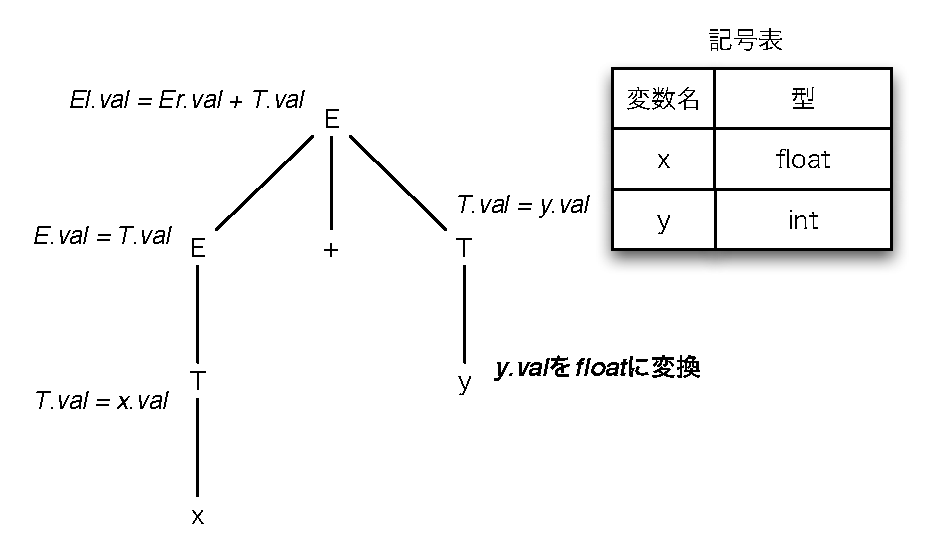
\includegraphics[width=12cm]{figure/type_conversion.pdf}
 \end{center}
 \caption{$B2r@OLZ$X$N7?JQ49>pJs$NIU2C(B}
 \label{191552_10Apr06}
\end{figure}

\section{$B2r@OLZ$rMQ$$$?0UL#2r@O(B}

$B2r@OLZ$rMQ$$$k$H!"$5$^$6$^$J<BMQE*$J=hM}$,BN7OE*$K9T$($k$h$&$K$J$k!#(B
\ref{163428_10Apr06}$B@a$G5s$2$?7?8!::$d(B\ref{190545_30Mar06}$B@a$G=R$Y$?;;=Q(B
$B<0$NCM$N7W;;$,$=$NNc$G$"$k!#K\@a$G$O!"$3$N$h$&$J2r@OLZ$rMQ$$$?0UL#2r@O$N(B
$B4pAC$H$J$kM}O@$H$7$F!"K]Lu%9%-!<%`$H$$$&9M$(J}$r>R2p$9$k!#(B

$B$^$:!"%3%s%Q%$%i$NF0:n$K6a$$Nc$H$7$F!"CfCV5-K!$G=q$+$l$?;;=Q<0$r8eCV5-K!(B
$B$KJQ49$9$k$3$H$r9M$($h$&!#(B

\subsection{$BCfCV5-K!$H8eCV5-K!(B}

$B2f!9$,IaCJL\$K$9$k(B2$B9`1i;;;R$O!"$?$$$F$$!"(B2$B$D$N1i;;?t$N4V$K1i;;;R$r=q$/!#(B
\icode{32 + 9}, \icode{4 / 2}$B$H$$$C$?6q9g$G$"$k!#$3$l$r(B{\bfseries $BCfCV5-(B
$BK!(B}$B!J(Binfix notation$B!K$H$$$&!#$7$+$7!";;=Q<0$N=q$-J}$O$3$l$@$1$G$O$J$$!#1i(B
$B;;;R$r(B2$B$D$N1i;;?t$NA0$KCV$/(B{\bfseries $BA0CV5-K!(B}$B!J(Bprefix notation$B!K!"(B2 $B$D(B
$B$N1i;;?t$N8e$m$KCV$/(B{\bfseries $B8eCV5-K!(B}$B!J(Bpostfix notation$B!K$H$$$&=q$-J}(B
$B$b$"$k!#$3$3$G$O8eCV5-K!$N$_$b$&>/$7>\$7$/@bL@$9$k$3$H$K$7$h$&!#(B

\begin{definition}
 $BCfCV5-K!$K$h$k<0(B$E$$B$N8eCV5-K!$O<!$N$h$&$K:F5"E*$KDj5A$5$l$k!#(B
 \begin{enumerate}
  \item $E$$B$,JQ?t$^$?$ODj?t$G$"$l$P!"(B$E$$B$N8eCV5-K!$O(B$E$$B$G$"$k!#(B
  \item $BG$0U$N(B2$B9`1i;;;R(B$\op$$B$K$D$$$F!"(B$E_1 \op E_2$$B$N8eCV5-K!$O(B
	$E_1'~E_2'~\op$$B$G$"$k!#$3$3$G(B$E_1', E_2'$$B$O$=$l$>$l(B$E_1, E_2$$B$N8e(B
	$BCV5-K!$G$"$k!#(B
  \item $(E)$$B$N8eCV5-K!$O(B$E'$$B$G$"$k!#$3$3$G(B$E'$$B$O(B$E$$B$N8eCV5-K!$G$"$k!#(B
 \end{enumerate}$\Box$
\end{definition}

\begin{example}
 $32 + 3$$B$N8eCV5-K!$O(B$32~3~+$$B$G$"$k!#(B$9 + 4 * 3$$B$N8eCV5-K!$O(B$9~4~3~*~+$$B$G(B
 $B$"$k!#(B$(1+2)*4$$B$N8eCV5-K!$O(B$1~2~+~4~*$$B$G$"$k!#(B$\Box$
 \label{ex:prefix_notation}
\end{example}

$B8eCV5-K!$G=q$+$l$?;;=Q<0$O!"%9%?%C%/(B1$B$D$G7W;;$G$-$k$H$$$&FCD'$r;}$D!#<0$r(B
$B:8$+$i1&$K(B1$B%H!<%/%s$:$DFI$_!"<!$NF0:n$r9T$($P$h$$!#(B
\begin{enumerate}
 \item $B%H!<%/%s$,?t$G$"$l$P!"$=$N?t$r%9%?%C%/$K@Q$`!J(Bpush$B!K!#(B
 \item $B%H!<%/%s$,1i;;;R(B$\op$$B$G$"$l$P!"%9%?%C%/$N>e(B2$B$D$NMWAG!J(B$x, y$$B$H$9$k!K(B
       $B$r$*$m$7!J(Bpop$B!K!"(B$x \op y$$B$r7W;;$7!"7k2L$r%9%?%C%/$K@Q$`!#(B
\end{enumerate}
$B$3$l$r<0$N=*$o$j$^$G9T$$!":G8e$K%9%?%C%/$K;D$C$??t$,<0$N7W;;7k2L$G$"$k!#(B
$BNc(B\ref{ex:prefix_notation}$B$N8eCV5-K!$G3N$+$a$F$_$h!#(B

\subsection{$BCfCV5-K!$+$i8eCV5-K!$X$NJQ49(B}

$BCfCV5-K!$G=q$+$l$?;;=Q<0$r8eCV5-K!$KJQ49$9$kJ}K!$N(B1$B$D$K!"2r@OLZ$rMQ$$$k$d(B
$B$jJ}$,$"$k!#J,$+$j$d$9$/$9$k$?$a$K!";;=Q<0$N$?$a$NJ8K!$H$7$F!"<!$N$h$&$J(B
$B!J:8:F5"$r4^$`!K$b$N$r9M$($k!#(B
\begin{equation}
\begin{split}
 E & \rightarrow E + E \\
 E & \rightarrow E - E \\
 E & \rightarrow E \ast E \\
 E & \rightarrow E\ /\ E \\
 E & \rightarrow (E) \\
 E & \rightarrow 0 \\
 \cdots \\
 E & \rightarrow 9
\end{split}\label{135829_4Apr06}
\end{equation}

\eqref{135829_4Apr06}$B$N5,B'$=$l$>$l$K%W%m%0%i%`CGJR$rIU$1$F$_$k!#$3$3$G(B
$putchar$$B$O!"0z?t$r0u;z$9$k4X?t$G$"$k!#(B
\begin{align*}
 E & \rightarrow E + E && \{ putchar('+'); \} \\
 E & \rightarrow E - E & & \{ putchar('-'); \} \\
 E & \rightarrow E \ast E & & \{ putchar('\ast'); \} \\
 E & \rightarrow E \ / \ E & & \{ putchar('/'); \} \\
 E & \rightarrow (E) & & \\ 
 E & \rightarrow 0 & & \{ putchar('0'); \} \\
 \cdots \\
 E & \rightarrow 9 & & \{ putchar('9'); \}
\end{align*}

\eqref{135829_4Apr06}$B$NJ8K!$K4p$E$$$F2r@OLZ$r:n$k$H$-!"F3=P$KMQ$$$?5,B'$K(B
$B%W%m%0%i%`CGJR$,IU$$$F$$$l$P!"$=$NCGJR$r:8JU$NHs=*C<5-9f$KBP1~$9$k@aE@$K(B
$BIU$1$F$*$/!#Nc$($P!"<0(B$(3+4)*5$$B$KBP$7$F%W%m%0%i%`CGJR$rIU$1$J$,$i2r@OLZ$r(B
$B:n$k$H!"?^(B\ref{142037_4Apr06}$B$N$h$&$K$J$k!#(B

\begin{figure}
 \begin{center}
  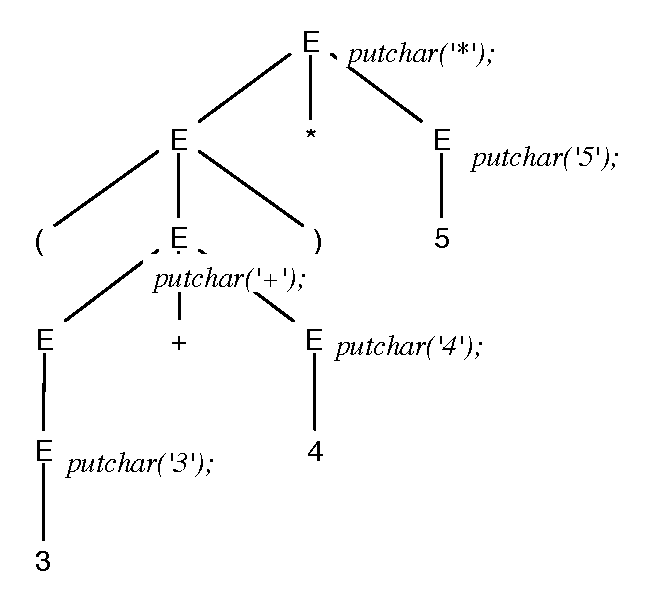
\includegraphics{figure/parse_tree_with_program.pdf}
 \end{center}
 \caption{$(3+4)*5$$B$KBP$9$k%W%m%0%i%`CGJRIU$-2r@OLZ(B}
 \label{142037_4Apr06}
\end{figure}

$BF@$i$l$?2r@OLZ$r?<$5M%@h$G$?$I$j!"@aE@$K%W%m%0%i%`CGJR$,IU$$$F$$$k>l9g$O(B
$B5"$j$,$1$K$=$NCGJR$r<B9T$9$k!#$9$k$H?^(B\ref{142037_4Apr06}$B$NNc$G$O(B
$3~4~+~5~*$$B$H$J$j!"8eCV5-K!$N<0$,@5$7$/F@$i$l$k!#(B

\section{$BK]Lu%9%-!<%`(B}
\label{195223_17Apr06}

$B?^(B\ref{142037_4Apr06}$B$NNc$G$O%W%m%0%i%`CGJR$r5"$j$,$1$K<B9T$7$?$,!"0lHL$K(B
$B$O!"9T$-$,$1$dDL$j$,$1$K%W%m%0%i%`CGJR$r<B9T$7$?$$$3$H$b$"$k!#$=$3$G!"(B
\eqref{135829_4Apr06}$B$N%W%m%0%i%`CGJRIU$-$NJ8K!$r>/$73HD%$7$h$&!#$3$l$,(B
{\bfseries $BK]Lu%9%-!<%`(B}$B$H8F$P$l$k$b$N$G$"$k!#(B

\begin{definition}
 $BJ8L.<+M3J8K!(B$G$$B$K$*$$$F!"(B$G$$B$N3F@8@.5,B'$N1&JU$K%W%m%0%i%`CGJR$rKd$a9~$s(B
 $B$GF@$i$l$k!J3HD%$5$l$?!KJ8K!$r(B{\bfseries $BK]Lu%9%-!<%`(B}$B!J(Btranslation
 scheme$B!K$H$$$&!#K]Lu%9%-!<%`$N4p$K$J$kJ8L.<+M3J8K!(B$G$$B$r(B{\bfseries $B4pDl(B
 $BJ8K!(B}$B!J(Bunderlying grammar$B!K!"Kd$a9~$^$l$?%W%m%0%i%`CGJR$r(B{\bfseries $B0U(B
 $BL#F0:n(B}$B!J(Bsemantic action$B!K$H$=$l$>$l8@$&!#(B$\Box$
\end{definition}

\begin{example}
 $B<!$K<($9$N$O!"4pDlJ8K!$r(B\eqref{135829_4Apr06}$B$H$7!"CfCV5-K!$N<0$r8eCV5-(B
 $BK!$KJQ49$9$kK]Lu%9%-!<%`$G$"$k!#(B
 \begin{equation}
\begin{split}
  E & \rightarrow E + E\ \{ putchar('+'); \} \\
  E & \rightarrow E - E\ \{ putchar('-'); \} \\
  E & \rightarrow E \ast E\ \{ putchar('*'); \} \\
  E & \rightarrow E\ /\ E\ \{ putchar('/'); \} \\
  E & \rightarrow (E) \\
  E & \rightarrow 0\ \{ putchar('0'); \} \\
  \cdots \\
  E & \rightarrow 9\ \{ putchar('9'); \}
\end{split}\label{151014_4Apr06} 
\end{equation}$\Box$
\end{example}

$B0UL#F0:n$rFC<l$J=*C<5-9f$H$_$J$9$H!"K]Lu%9%-!<%`$OJ8L.<+M3J8K!$H8+$k$3$H(B
$B$,$G$-!"!J0UL#F0:n$r4^$s$@!K2r@OLZ$r@8@.$7$?$j!":8:F5"$N=|5n$J$I$NJ8L.<+(B
$BM3J8K!$NJQ7A<jK!$r$=$N$^$^E,MQ$7$?$j$G$-$k!#(B

\begin{example}
 \eqref{151014_4Apr06}$B$NK]Lu%9%-!<%`$rMQ$$$F<0(B$4 + 3 * 5$$B$N!J0UL#F0:n$r4^(B
 $B$s$@!K2r@OLZ$r@8@.$9$k$H?^(B\ref{152516_4Apr06}$B$N$h$&$K$J$k!#$3$N2r@OLZ$r(B
 $B?<$5M%@h$K$?$I$j!"0UL#F0:n$N@aE@$G$O$=$N0UL#F0:n$r<B9T$9$k$H!"<0(B
 $4~3~5~\ast~+$$B$H$$$&8eCV5-K!$N<0$,F@$i$l$k!#(B
\end{example}

\begin{figure}
 \begin{center}
  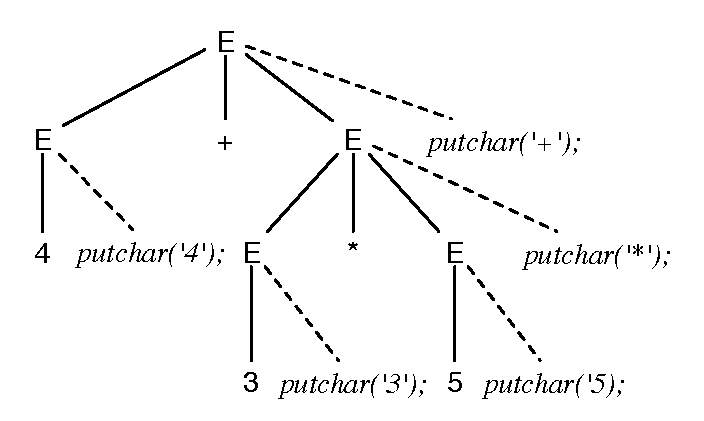
\includegraphics{figure/translation_scheme_parse_tree.pdf}
 \end{center}
 \caption{$BK]Lu%9%-!<%`$K$h$k(B$4+3*5$$B$N2r@OLZ(B}
 \label{152516_4Apr06}
\end{figure}

\begin{example}
 \eqref{151014_4Apr06}$B$NK]Lu%9%-!<%`$K(B\ref{121145_31Mar06}$B$N<jK!$rE,MQ$7(B
 $B$F:8:F5"$r=|5n$9$k$H!"<!$N$h$&$JK]Lu%9%-!<%`$KJQ7A$5$l$k!#(B
 \begin{align*}
  E \rightarrow & (E)E' \\
     & \mid 0\ \{ putchar('0'); \}\ E' \\ 
     & \mid \cdots \\
     & \mid 9\ \{ putchar('9'); \}\ E' \\
  E' \rightarrow & +E\ \{ putchar('+'); \}\ E' \\
     & \mid -E\ \{ putchar('-'); \}\ E' \\
     & \mid \ast E\ \{ putchar('\ast'); \}\ E' \\
     & \mid /E\ \{ putchar('/'); \}\ E' \\
     & \mid \epsilon
 \end{align*}
 $B$3$l$rMQ$$$F<0(B$3 * (1 + 2)$$B$N2r@OLZ$r@8@.$9$k$H?^(B\ref{155248_4Apr06}$B$N$h(B
 $B$&$K$J$k!#(B
\end{example}

\begin{figure}
 \begin{center}
  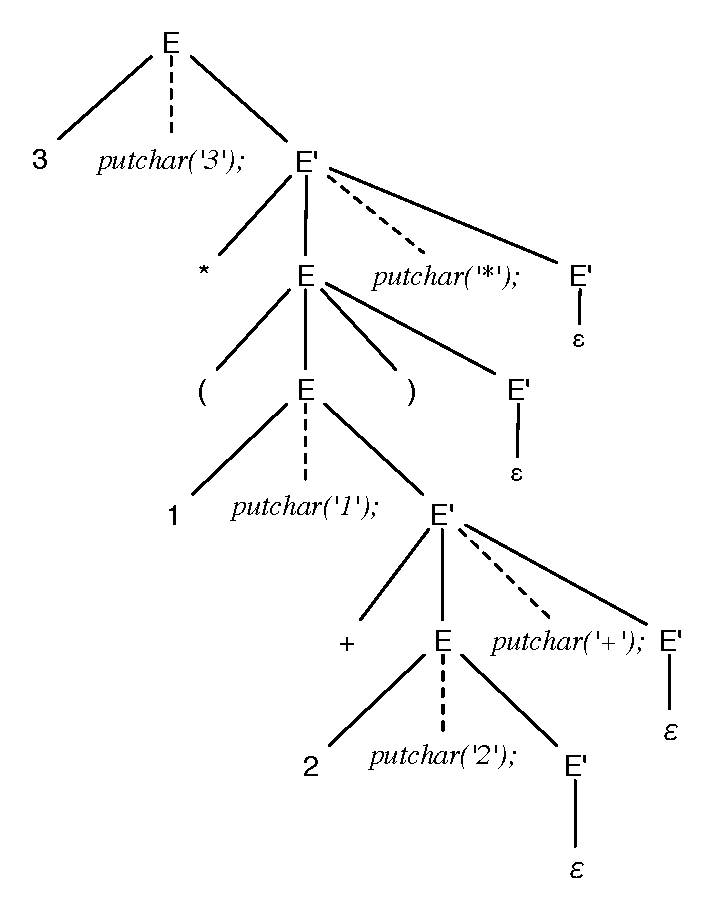
\includegraphics{figure/translation_scheme_no_left_recurs.pdf}
 \end{center}
 \caption{\eqref{151014_4Apr06}$B$K$h$k(B$3 * (1 + 2)$$B$N2r@OLZ(B}
 \label{155248_4Apr06}
\end{figure}

\subsection{$B0UL#F0:n$N7A<0(B}

$B0J9_$N@a$N=`Hw$H$7$F!"0UL#F0:n$N7A<0$K$D$$$F$b$&>/$7>\$7$/=R$Y$k!#$3$l$^(B
$B$G!"0UL#F0:n$O%W%m%0%i%`CGJR$@$H$7$F$-$?$,!"$I$s$J7A$N%W%m%0%i%`$G$bG'$a(B
$B$i$l$k$o$1$G$O$J$$!#;H$($kJQ?t$K4X$7$F@)8B$,$"$k!#(B

$B%W%m%0%i%`CGJRCf$G;H$($kJQ?t$O(B$X.v$$B$H$$$&7A<0$K8B$i$l$k!#$3$3$G(B$X$$B$O!"4p(B
$BDlJ8K!$K=P8=$9$kHs=*C<5-9f$^$?$O=*C<5-9f$G$"$k!#(B$v$$B$OK]Lu%9%-!<%`Fb$GE,Ev(B
$B$K7h$a$F9=$o$J$$!#(B$v$$B$r(B$X$$B$N(B{\bfseries $BB0@-(B}$B!J(Battribute$B!K$H$$$&!#(B

\section{$B@-<A$N$h$$K]Lu%9%-!<%`(B}

$BA0@a$G=R$Y$?K]Lu%9%-!<%`$K$h$k7W;;$O!">o$K8zN($h$/9T$($k$o$1$G$O$J$$!#7W(B
$B;;8zN($N%]%$%s%H$N0l$D$,!V?<$5M%@h$K(B1$B2s$?$I$k$@$1$G7W;;$G$-$k$+!W$G$"$k!#(B
$B2r@OLZ$O0lHL$KBg$-$/$J$j$,$A$J$N$G!"?<$5M%@hC5:w$N2s?t$,A}$($k$[$I!"7W;;(B
$B8zN($,0-$/$J$k$3$H$,M=A[$5$l$k$+$i$G$"$k!#(B

$B$=$3$G$3$N@a$G$O!"K]Lu%9%-!<%`$N0UL#F0:n$K@)8B$r2C$(!"?<$5M%@h$K(B1$B2s$?$I$k(B
$B$@$1$G7W;;$,9T$($kK]Lu%9%-!<%`!J(BS$BB0@-Dj5A!"(BL$BB0@-Dj5A!K$rF3F~$9$k!#(B

\subsection{$B9g@.B0@-$HAjB3B0@-(B}

$B$b$H$b$H$NK]Lu%9%-!<%`$G$O!"4pDlJ8K!$K=P8=$9$kHs=*C<5-9f$d=*C<5-9f$NB0@-(B
$B$O$9$Y$F0UL#F0:nFb$GMQ$$$k$3$H$,$G$-$k!#$7$+$7!"$3$l$G$O0UL#F0:n$N1&JUCM(B
$B!J(B$v=E$$B$N7A$NJ8$N(B$E$$B!K$r7W;;$9$k$N$K!"2r@OLZ$N$"$A$3$A$r;2>H$7$J$/$F$O$J(B
$B$i$:!"?<$5M%@h$K(B1$B2s$?$I$k$@$1$G$OE~Dl7W;;$,=*$o$i$J$$!#(B

$B$=$3$G!"@-<A$N$h$$B0@-$r(B2$B$DDj5A$7$h$&!#(B
\begin{definition}
 $B2r@OLZ$N@aE@(B$A$$B$K$D$$$F!"(B$A$$B$NB0@-(B$x$$B$,(B$A.x = f(c_1, c_2, \cdots, c_n)$
 $B$H7W;;$G$-$k$H$9$k!#(B$c_1, c_2, \cdots, c_n$$B$,$9$Y$F(B$A$$B$N;R(B
 $B@aE@$NB0@-$G$"$k$H$-!"(B$x$$B$r(B$A$$B$N(B{\bfseries $B9g@.B0@-(B}$B!J(Bsynthesized
 attribute$B!K$H$$$&!#(B$\Box$
\end{definition}

\begin{definition}
 $B2r@OLZ$N@aE@(B$A$$B$K$D$$$F!"(B$A$$B$NB0@-(B$x$$B$,(B$A.x = f(c_1, c_2, \cdots, c_n)$
 $B$H7W;;$G$-$k$H$9$k!#(B$c_1, c_2, \cdots, c_n$$B$,$9$Y$F(B$A$$B$N?F@aE@$^$?$O7;Do(B
 $B@aE@$NB0@-$G$"$k$H$-!"(B$x$$B$r(B$A$$B$N(B{\bfseries $BAjB3B0@-(B}$B!J(Binherited
 attribute$B!K$H$$$&!#(B$\Box$
\end{definition}

$B@8@.5,B'(B$A \rightarrow \alpha$$B$K4p$E$$$F@bL@$9$k$H!"<!$N$h$&$K$J$k!#(B
\begin{itemize}
 \item $A$$B$NB0@-(B$x$$B$,(B$\alpha$$BCf$NHs=*C<5-9f$d=*C<5-9f$NB0@-$N$_$+$i7W;;$G(B
       $B$-$k$J$i!"(B$x$$B$O9g@.B0@-(B
 \item $\alpha$$BCf$N5-9f(B$B$$B$NB0@-(B$y$$B$,!"(B$A$$B$d(B$\alpha$$BCf$NB>$N5-9f$NB0@-$N(B
       $B$_$+$i7W;;$G$-$k$J$i!"(B$y$$B$OAjB3B0@-(B
\end{itemize}

\begin{example}
 $B<!$K<($9K]Lu%9%-!<%`$O9g@.B0@-$N$_$+$i$J$k!#E:;z$N(B$l, r$$B$O!"$=$l$>$l:8JU(B
 $B$K=P8=$9$k5-9f!"1&JU$K=P8=$9$k5-9f$rI=$7$F$$$k!#(B
 \begin{align*}
 E & \rightarrow E + T && \{ E_l.val = E_r.val + T.val; \} \\
 E & \rightarrow T && \{E.val = T.val; \} \\
 T & \rightarrow T * F && \{ T_l.val = T_r.val * F.val; \} \\
 T & \rightarrow F && \{ T.val = F.val; \} \\
 F & \rightarrow (E) && \{ F.val = E.val; \} \\
 F & \rightarrow digit && \{ F.val = digit.lexval; \}
 \end{align*}$\Box$
 \label{example:S-attributed definition}
\end{example}

\begin{example}
 $B<!$K<($9K]Lu%9%-!<%`$N$&$A!"Hs=*C<5-9f(B$L$$B$NB0@-(B$in$$B$OAjB3B0@-$G$"$k!#(B
 \begin{align*}
 D & \rightarrow T\ L && \{ L.in = T.type; \} \\
 T & \rightarrow int && \{ T.type = integer; \} \\
 T & \rightarrow float && \{ T.type = float; \} \\
 L & \rightarrow L, id	&& \{ L_r.in = L_l.in; addtype(id.entry, L_l.in); \} \\
 L & \rightarrow id && \{ addtype(id.entry, L.in); \}
 \end{align*}$\Box$
 \label{example:L-attributed definition}
\end{example}

$B9g@.B0@-$dAjB3B0@-$O!"2r@OLZ$N?<$5M%@hC5:w$HAj@-$,NI$$!#9g@.B0@-$N7W;;$O!"(B
$B5"$j$,$1$K9T$&$H$?$I$j$r(B1$B2s$G:Q$^$;$k$3$H$,$G$-$k!#$^$?!"AjB3B0@-$N0lIt$b!"(B
1$B2s$N$?$I$j$G7W;;$r9T$&$3$H$,$G$-$k!#(B

\subsection{S$BB0@-Dj5A(B}

\begin{definition}
 $BK]Lu%9%-!<%`$N$&$A!"<!$N>r7o$rK~$?$9$b$N$r(B{\bfseries S$BB0@-Dj(B
 $B5A(B}$B!J(BS-attributed definition$B!K$H$$$&!#(B
 \begin{enumerate}
  \item $B0UL#F0:nCf$K8=$l$kJQ?t$O$9$Y$F9g@.B0@-$G$"$k!#(B
  \item $B$9$Y$F$N0UL#F0:n$O!"@8@.5,B'$N1&JU$NKvHx$K$7$+8=$l$J$$!#(B
 \end{enumerate}$\Box$
\end{definition}

\begin{example}
 $BNc(B\ref{example:S-attributed definition}$B$NK]Lu%9%-!<%`$O(BS$BB0@-Dj5A$G$"$k!#(B
 $\Box$
\end{example}

$BDj5A$h$j!"(BS$BB0@-Dj5A$N0UL#F0:n$O!"2r@OLZ$r(B1$B2s?<$5M%@h$K$?$I$k$@$1$G$9$Y$F(B
$B7W;;$9$k$3$H$,$G$-$k!#(B

\subsection{L$BB0@-Dj5A(B}

\begin{definition}
 $BK]Lu%9%-!<%`$N$&$A!"<!$N>r7o$rK~$?$9$b$N$r(B{\bfseries L$BB0@-Dj(B
 $B5A(B}$B!J(BL-attributed definition$B!K$H$$$&!#(B
 \begin{enumerate}
  \item $B0UL#F0:nCf$K8=$l$kJQ?t$O$9$Y$F9g@.B0@-$+AjB3B0@-$G$"$k!#(B
	\label{153250_7Apr06}
  \item $B4pDlJ8K!$N@8@.5,B'(B$A \rightarrow X_1X_2\cdots X_n$$B$K$D$$$F!"(B
	$X_j$$B$NAjB3B0@-$O!"(B$X_1, X_2, \cdots, X_{j-1}$$B$NB0@-$H(B$A$$B$NAjB3B0(B
	$B@-$@$1$K0MB8$9$k!#(B
  \item $B4pDlJ8K!$N@8@.5,B'(B$A \rightarrow X_1X_2\cdots X_n$$B$K$D$$$F!"(B
	$X_j$$B$NAjB3B0@-$r:8JU$K;}$DJ8$r4^$`0UL#F0:n$O!"(B$X_j$$B$ND>A0$K=P8=(B
	$B$9$k!#(B
  \item $B4pDlJ8K!$N@8@.5,B'(B$A \rightarrow X_1X_2\cdots X_n$$B$K$D$$$F!"(B$A$$B$N(B
	$B9g@.B0@-$O$3$N5,B'$NKvHx$K=P8=$9$k!#(B
	\label{153257_7Apr06}
 \end{enumerate}$\Box$
 \label{def:L-attributed definition}
\end{definition}

\begin{example}
 $B<!$NK]Lu%9%-!<%`$O(BL$BB0@-Dj5A$G$"$k!#$3$3$G!"(B$type$$B$O9g@.B0@-!"(B$in$$B$OAjB3(B
 $BB0@-$G$"$k(B\footnote{$B$3$NK]Lu%9%-!<%`$O!"(B\icode{int i, j;} $B$N$h$&$K(B
 \icode{int}$B7?$NJQ?t$rJ#?tF1;~$K@k8@$9$k$H$-$K!"(B\icode{i}, \icode{j}$B$N7?(B
 $B$r(B\icode{int} $B$HDj$a$k$b$N$G$"$k!#(B}$B!#$^$?(B$entry$$B$O<1JL;R$rI=$9=*C<5-9f(B
 $id$$B$NB0@-$G$"$j!"$=$N<1JL;R$NL>A0$r3JG<$7$F$$$k$H$9$k!#(B$entry$$B$NCM$O0U(B
 $BL#2r@O0JA0$K$9$G$KJ,$+$C$F$$$k$b$N$H$9$k!#4X?t(B$addtype(id.entry, L.in)$
 $B$O!"(B$id.entry$$B$N7?$H$7$F(B$L.in$$B$rEPO?$9$k!"$H$$$&F0:n$r$9$k!#(B
 \begin{align*}
  D & \rightarrow T\ \{ L.in = T.type; \}\ L \\
  T & \rightarrow \icode{int}\ \{ T.type = integer; \} \\
  T & \rightarrow \icode{float}\ \{ T.type = float; \} \\
  L & \rightarrow \{ L_r.in = L_l.in; \}\ L\ \icode{,}\ \icode{id}\ \{ addtype(\icode{id}.entry, L_l.in); \}\\
  L & \rightarrow \icode{id}\ \{ addtype(\icode{id}.entry, L.in); \}
 \end{align*}$\Box$
 \label{example:L-attributed translation scheme}
\end{example}

$BDj5A(B\ref{def:L-attributed definition}$B$N(B\ref{153250_7Apr06}$B$H(B
\ref{153257_7Apr06}$B$+$iJ,$+$k$h$&$K!"$b$7(BL$BB0@-Dj5A$KAjB3B0@-$,0l$D$b4^$^(B
$B$l$J$1$l$P!"(BS$BB0@-Dj5A$=$N$b$N$G$"$k!#$9$J$o$A!"(BS$BB0@-Dj5A$OI,$:(BL$BB0@-Dj5A$K(B
$B$J$k!#(B

S$BB0@-Dj5A$HF1MM$K!"(BL$BB0@-Dj5A$NK]Lu%9%-!<%`$b2r@OLZ$r(B1$B2s?<$5M%@h$K$?$I$k$@(B
$B$1$G!"$9$Y$F$N0UL#F0:n$r7W;;$9$k$3$H$,$G$-$k!#(B

\begin{figure}
 \begin{center}
  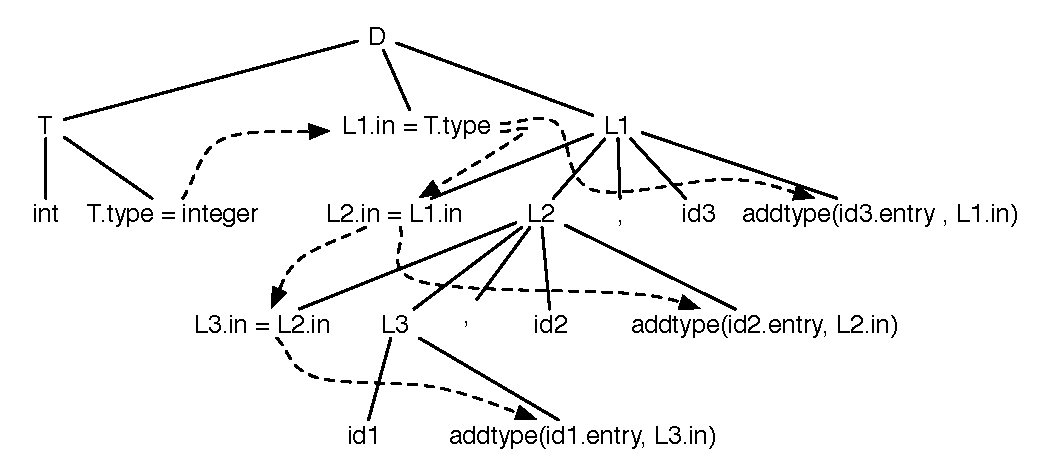
\includegraphics[width=13cm]{figure/L_attr_translation_scheme.pdf}
 \end{center}
 \caption{L$BB0@-Dj5A$K4p$E$/2r@OLZ(B}
 \label{170525_7Apr06}
\end{figure}

\begin{example}
 $BNc(B\ref{example:L-attributed translation scheme}$B$NK]Lu%9%-!<%`$K4p$E$$$F!"(B
 $B%H!<%/%sNs(B\icode{int id, id, id}$B$+$i@8@.$7$?0UL#F0:nIU$-2r@OLZ$r?^(B
 \ref{170525_7Apr06}$B$K<($9!#$J$*!"Hs=*C<5-9f(B$L$$B!"=*C<5-9f(B$id$$B$,J#?t8=$l$k(B
 $B$N$G!"JX59>eE:;z$rIU$1$F6hJL$7$F$$$k!#(B

 $B?^Cf$NGK@~$O!"B0@-$N0MB84X78$r<($7$F$$$k!#Nc$($P!"0UL#5,B'(B$T.type =
 integer;$$B$G7hDj$7$?(B$T.type$$B$NCM$r(B$L_1.in = T.type;$$B$G;2>H$9$k!"$H$$$C$?(B
 $B6q9g$G$"$k!#$3$N2r@OLZ$r?<$5M%@h$G$?$I$C$F$$$/$H!"GK@~$G<($7$?B0@-$N0MB8(B
 $B4X78$N=g=x$r<i$j$J$,$i0UL#5,B'$,7W;;$5$l$F$$$/$3$H$r3N$+$a$h!#(B$\Box$
\end{example}

% \section{$BK]Lu%9%-!<%`$r<B9T$9$k%W%m%0%i%`$N@8@.(B}

% $B0lHL$K$O!"K]Lu%9%-!<%`$r<B9T$9$k%W%m%0%i%`$r@8@.$9$k$N$OC1=c$G$O$J$$!#$7(B
% $B$+$7!"4pDlJ8K!$r(BLL(1)$BJ8K!$J$IM=B,7?9=J82r@O$N9T$($kJ8K!$K@)8B$7!"$+$DK]Lu(B
% $B%9%-!<%`$r(BS$BB0@-Dj5A!&(BL$BB0@-Dj5A$K@)8B$9$k$H!"K]Lu%9%-!<%`$r<B9T$9$k%W%m%0(B
% $B%i%`$O<+F0@8@.$G$-$k!#(B

% $BM=B,7?9=J82r@O%k!<%A%s$O<!$N$h$&$K@8@.$9$k$N$G$"$C$?!#(B
% \begin{enumerate}
%  \item $B3FHs=*C<5-9f$KBP1~$9$k4X?t$rMQ0U$9$k(B
%  \item $B$=$N4X?tFb$K!"@8@.5,B'$N1&JU$K$J$i$C$F!"@aE@$N@8@.$dHs=*C<5-9f$KBP(B
%        $B1~$9$k4X?t8F$S=P$7$rJB$Y$k(B
%        \label{153525_10Apr06}
% \end{enumerate}
% $B$3$l$r<B9T$9$k$H!"$"$?$+$b2r@OLZ$r?<$5M%@h$K$?$I$k$h$&$K=hM}$,9T$o$l$k!#(B

% $B$=$3$G!"(B\ref{153525_10Apr06}$B$r9T$&$H$-$K!"0UL#F0:n$rBP1~$9$k>l=j$KKd$a9~(B
% $B$`!#$9$k$H!"F@$i$l$?M=B,7?9=J82r@O%k!<%A%s$r<B9T$9$k$H!"2r@OLZ$r?<$5M%@h(B
% $B$G$?$I$j$J$,$iBP1~$9$k0UL#F0:n$,<B9T$5$l!"(BS$BB0@-Dj5A$d(BL$BB0@-Dj5A$G$"$l$P@5(B
% $B$7$/=hM}$5$l$k$3$H$K$J$k!#(B

% $B$?$@$7!"(B

% - [ ] $BM=B,7?9=J82r@O$X$NK]Lu%9%-!<%`$NKd$a9~$_(B
% 	- [ ] $BNc!'(B2-13$B!J9g@.B0@-$bAjB3B0@-$b4^$^$l$F$$$J$$!K(B
% 	- [ ] $B:8:F5"$N=|5n(B
% 		- [ ] $B@8@.5,B'$NCf$KKd$a9~$s$@0UL#F0:n$b0l=o$K9T$&(B
% 		- [ ] 2-13 $B"*(B 2-14$B!"K]Lu$NMM;R!'?^(B2.21
% 	- [ ] $BK]Lu%W%m%0%i%`$N@8@.(B
% 		- [ ] $BM=B,7?9=J82r@O$HF1MM(B
% 		- [ ] $B0UL#F0:n$KBP1~$9$k>l=j$K!"0UL#F0:n$N%W%m%0%i%`JR$r$=$N$^$^Kd$a9~$`(B
% 		- [ ] $B7k2L!'(B2-22
% - [ ] $B0lHLE*$JK]Lu%9%-!<%`$NKd$a9~$_(B
% 	- [ ] $B9g@.B0@-$bAjB3B0@-$b4^$^$l$k>l9g(B
% 	- [ ] $B%]%$%s%H!'0UL#F0:n$NCf$G;2>H$9$kB0@-$O!"$=$NF0:n$r<B9T$9$k;~E@$G$O$9$G$KI>2A$7=*$o$C$F$$$J$1$l$P$J$i$J$$!JCM$,5a$^$C$F$$$J$1$l$P$J$i$J$$!K(B
% 		- [ ] $B@8@.5,B'$N1&JU$N5-9f$NAjB3B0@-!'$=$N5-9f$h$jA0$NF0:n$GCM$,5a$a$i$l$F$$$J$1$l$P$J$i$J$$(B
% 		- [ ] $B3FF0:n$NCf$G$O!"$=$NF0:n$h$j1&$K$"$k5-9f$N9g@.B0@-$r;2>H$7$F$O$$$1$J$$(B
% 		- [ ] $B@8@.5,B'$N:8JU$NHs=*C<5-9f$N9g@.B0@-!';2>H$9$kB0@-$r$9$Y$F7W;;$7$?8e!"7W;;$9$k!J0UL#F0:n$r@8@.5,B'$N1&JU$N:G8e$KCV$/!K(B
% 	* [ ] $B9=J8<gF3Dj5A$+$iK]Lu%9%-!<%`$r:n$k$K$O(B
% 	- [ ] $B:8:F5"$N=|5n(B
% 		- [ ] $B>e$N(B3$B$D$N>r7o$rK~$?$9$h$&$K!"0UL#F0:n$rJQ7A$7$J$1$l$P$J$i$J$$(B
% 		- [ ] 5-24$B"*(B 5-25
% 			- [ ] $B?7$?$KF3F~$5$l$?Hs=*C<5-9f(B R, R1$B$NB0@-(B i, s
% 		- [ ] $BCj>]E*$K$O(B
% 			- [ ] $BK]Lu%9%-!<%`JQ49(B
% 			- [ ] $BB0@-CM$N5a$aJ}$N0c$$!'?^(B5.27
% 		- [ ] $BM=B,7?9=J82r@O%k!<%A%s!\K]Lu%9%-!<%`Kd$a9~$_!!$N@8@.(B
% 			- [ ] $BHs=*C<5-9f(BA$B$KBP$9$k4X?t(B A()
% 				- [ ] A$B$NAjB3B0@-$r2>0z?t$K(B
% 				- [ ] A$B$N9g@.B0@-$rJV$jCM$K(B
% 				- [ ] A$B$r:8JU$H$9$k@8@.5,B'$K8=$l$k5-9f$NB0@-$r6I=jJQ?t$K(B
% 			- [ ] $B@8@.5,B'$N1&JU$r:8$+$i1&$KD4$Y(B
% 				- [ ] $B9g@.B0@-(B x $B$r;}$D%H!<%/%s!J=*C<5-9f!K(BX
% 					- [ ] X.x$B$KBP1~$9$kJQ?t(B = X.x$B$NCM(B; X$B$H$N>H9g(B; $BF~NO$r@h$K?J$a$k(B;
% 				- [ ] $BHs=*C<5-9f(BB
% 					- [ ] B$B$N9g@.B0@-$KBP1~$9$kJQ?t(B = B(b1, b2, $B!D(B, bk);
% 						- [ ] b1, b2, $B!D(B, bk$B!'(BB$B$NAjB3B0@-$KBP1~$9$kJQ?t(B
% 				- [ ] $B0UL#F0:n(B
% 					- [ ] $B%W%m%0%i%`JR$rJ#<L!JB0@-$N;2>H$O!"BP1~$9$kJQ?t$N;2>H$KCV$-49$(!K(B
% 			- [ ] $BNc!'(B5-31


%#!platex main

\chapter{実行時環境}
\label{083441_12Apr06}
% 7.3節まで

以降の章では、意味解析部までで得られた解析木をもとに機械語命令列を生成す
る部分({\bf コード生成部})について説明を行う。

実際に生成される機械語命令列は、対象とするCPUによって異なる。したがって、
コード生成部の詳細は、対象とするCPUによっても異なってくる。ここでは、具体
性を持たせるために、Pentiumプロセッサを対象とし、また\icode{gcc}コンパイ
ラで生成されるアセンブリ言語を例として用いる。ただし、説明する手法は特定
のCPUに依存しない汎用的なものである。

CやML, Javaのように、我々が通常プログラミングを行う言語を高級言語というこ
とがある。これは、アセンブリ言語や機械語に比べて論理的に高度な概念が扱え
ることに由来する用語である。例えば、関数、型、構造体などはすべて高級言語
にしかない「高度な概念」と言える。

本講義を受講している諸君は、すでにCなどの高級言語によるプログラミングは充
分習得していることであろう。また、アセンブリ言語や、それをCPUがいかにして
実行するかも学習していることであろう\footnote{計算機アーキテクチャA}。し
かし、この2つのプログラム実行の間には、論理的に大きな差がある。例えば、C
言語の関数の呼び出し、実行、返り値の処理などが、一体どういう機械語列にな
り、どのように実行されているのか、想像がつくだろうか。このギャップを埋め、
コード生成の理解のための準備をするのが、本章の目的である。

\section{予備知識}

\subsection{メモリ領域}

我々が今日用いる汎用コンピュータは、プログラムの機械語列やデータをメモリ
上に置き、その機械語列をCPUが実行していく、という形式のものがほとんどであ
る。プログラムの機械語列もメモリ上に置かれているため、メモリ上の機械語列
を置き換えるだけで、違うプログラムが実行できる\footnote{このようなコン
ピュータのことを{\bf フォン・ノイマン型計算機}という。}。メモリは通常1バ
イト単位で読み書きが可能であり、各バイトには一意に定まる番号が振られてい
る。この番号のことを{\bf 番地}(アドレス、address)という。番地は0番から
始まり、例えば32ビット計算機であれば$2^{32}-1$番地までである。

メモリはいくつかの連続した領域({\bf メモリ領域})に分割して使用される。
\begin{itemize}
 \item OS専用の領域。個々の計算機、OSごとに大きさは固定されている。
 \item {\bfseries ユーザ領域}…通常のプログラムを実行するのに使用される領域
       \begin{itemize}
	\item {\bfseries コード領域}…実行するプログラムを格納する領域。
	      いったんプログラムがメモリ上にロードされれば、変更されない。
	      すなわち、読み取り専用の領域である。
	\item {\bfseries データ領域}…プログラム実行に必要なデータを格納
	      する領域。プログラムの実行とともに内容が変化する。すなわち
	      読み書き可能な領域である。
	      \begin{itemize}
	       \item {\bfseries 大域データ領域}…大域変数を割り当てる領域
	       \item {\bfseries 実行時スタック}…局所変数や関数への実引数
		     を割り当てる領域
	       \item {\bfseries ヒープ}…\icode{malloc()}などにより実行時
		     に動的に生成されるデータを割り当てる領域
	      \end{itemize}
       \end{itemize}
\end{itemize}

\begin{figure}
 \begin{center}
  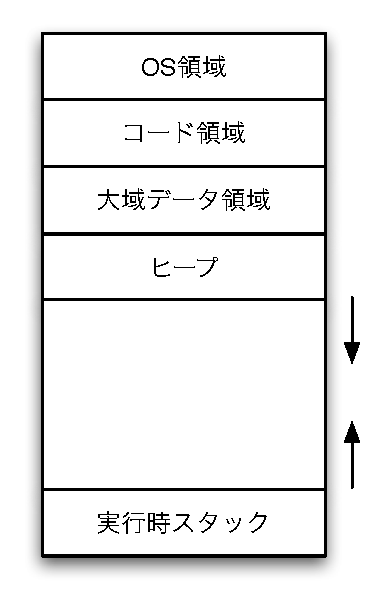
\includegraphics{figure/memory_area.pdf}
 \end{center}
 \caption{メモリ領域の分割例}
 \label{104220_11Apr06}
\end{figure}

ユーザ領域のうち、コード領域と大域データ領域の大きさはコンパイル時に決定
され、プログラム実行時には変化しない。一方、実行時スタックとヒープの大き
さは実行時に変化する。このような性質を満たすようなメモリ領域の使い方の一
例を図\ref{104220_11Apr06}に示す。この例では、メモリの下位番地からOS領域、
コード領域、大域データ領域、ヒープを割り当て、実行時スタックは逆にメモリ
の上位番地から割り当てる。

大域変数が割り当てられる番地はコンパイル時に決定される\footnote{現代のコ
ンピュータでは、複数のプログラムを同時に実行させることができる。そのため、
実際には、コード領域や大域データ領域についても、コード領域の先頭からの相
対番地のみ決定しておき、プログラム(機械語命令列)をメモリ上のどこにも配
置できるようにしておくことが多い。このような機械語命令列のことを
{\bfseries 再配置可能}(relocatable)であると言う。}。一方局所変数や実引
数は、プログラム実行中に関数が呼び出されたとき、実行時スタック上に割り当
てられるので、それまで番地は決定できない。また\icode{malloc()}などにより
動的に確保された領域も、実行時に実際にヒープに割り当てられるまで、番地は
決定できない。

\subsection{CPUとレジスタ}

メモリ上に配置された機械語プログラムはCPU(中央演算処理装置)が実行する。
具体的には、機械語プログラムを順に1命令ずつ読み出し、その命令に書かれた指
示に従ってメモリ領域やレジスタから値を読み出して算術演算や比較演算を行い、
結果をメモリ領域やレジスタに格納する。これを繰り返す。

Pentiumプロセッサには、次のようなレジスタが用意されている。
\begin{enumerate}
 \item {\bfseries 汎用レジスタ}(general-purpose register)…算術演算や
       比較演算などの演算数として用いることのできるレジスタ。本講義での
       機械語命令には、\icode{\%eax}, \icode{\%ebx}, \icode{\%ecx},
       \icode{\%edx}などのレジスタの他、実行時スタックを操作するのに用い
       られる{\bfseries ベースポインタ}(base pointer)\icode{\%ebp}と
       {\bfseries スタックポインタ}(stack pointer)\icode{\%esp}がある。
 \item {\bfseries 条件フラグ}(condition flag)…比較命令の結果を格納する
       レジスタ。ゼロフラグ\icode{\%zf}や符号フラグ\icode{\%sf}などがある。
       本講義で扱う機械語命令では、比較命令が自動的に設定し、条件付きジャ
       ンプ命令が適切なフラグを自動的に参照する。したがって、機械語命令に
       明示的に現れることはない。
 \item {\bfseries 命令ポインタ}(instruction pointer)…{\bfseries プログ
       ラムカウンタ}(program counter)とも言う。CPUが次に実行すべき命令
       の格納番地を指すレジスタ。\icode{\%eip}という記法を用いる。この値
       も自動的に更新されるため、命令ポインタが機械語命令に明示的に現れる
       ことはない。
\end{enumerate}

\subsection{機械語命令}

以降の説明を理解するのに必要な機械語命令について、簡単にまとめておく。な
お、本講義では Pentium プロセッサの機械語を記述するのに、AT\&T形式と呼ば
れるアセンブリ言語を用いている。

個々の機械語命令は、次のような書式をしている。[]は、その部分が省略可能で
あることを表している。
\begin{quote}
 [ラベル:] 命令名 第1演算数[, 第2演算数, $\cdots$, 第$n$演算数]
\end{quote}

ラベルは、コード領域中でこの機械語命令が置かれている番地を表すためのシン
ボルであり、先頭が\icode{\underline{ }}であるような文字列を用いる。関数に
相当する機械語命令列の先頭には、\icode{\underline{ }関数名}というラベルが
必ず付けられる。なお、図\ref{143232_11Apr06}の3行目のように、ラベルだけが
1行に書かれていても構わない。

演算数として用いることのできるのは、汎用レジスタ、メモリ番地、整数定数の
みである\footnote{整数定数以外の定数(文字列、浮動小数点数など)は、コー
ド領域や大域データ領域などに値を格納しておき、その番地をラベルで参照す
る。}。メモリ番地の指定は、以下の2通りの方法がある。
\begin{enumerate}
 \item その番地に付けられたラベル名
 \item 汎用レジスタの値を番地と見なし、その番地からの相対番地を指定する。
       例えば、$(レジスタRの値)$番地を$(\%R)$、$(レジスタRの値 + n)$番地
       を$n(\%R)$というように記述する。括弧がつくことで、レジスタそのもの
       ではなく、レジスタの値の番地という意味になることに注意してほしい
       \footnote{間接参照という。}。
\end{enumerate}
また整数定数の先頭には\$を付ける。

本講義では、実際の Pentium プロセッサの機械語のうちごく一部だけを用いる。
\begin{description}
 \item[2項算術命令] 演算数を2つとる算術演算。\icode{addl}(加算),
	    \icode{subl}(減算), \icode{imull}(乗算)などがある。結果は
	    第2演算数に格納される。例えば\icode{add~\%ebx,\%eax}は、レジ
	    スタ\icode{\%ebx}の値をレジスタ\icode{\%eax}の値に加え、結果
	    をレジスタ\icode{\%eax}に格納する。
 \item[単項算術命令] 演算数を1つとる算術演算。\icode{neg}(符号の反転)、
	    \icode{dec}(1引く)、\icode{inc}(1足す)などがある。結果は
	    第1演算数に格納される。例えば\icode{inc~\%eax}は、レジスタ
	    \icode{\%eax}の値に1を加え、結果を\icode{\%eax}に格納する。
 \item[移動命令] 演算数を2つとり、第1演算数の値を第2演算数に格納する。本
	    講義では\icode{movl}のみ扱う。例えば\icode{movl~\%eax,\%ebx}
	    は、レジスタ\icode{\%eax}の値をレジスタ\icode{\%ebx}に格納す
	    る。
 \item[比較命令] 演算数を2つとり、第1演算数と第2演算数を比較し、結果を条
	    件フラグに設定する。定数は第1演算数でのみ使える。本講義では
	    \icode{cmpl}のみ用いる。例えば\icode{cmpl~\$4,\%eax}は、定数4と
	    レジスタ\icode{\%eax}の値とを比較し、次のように条件フラグを設
	    定する。
	    \begin{align*}
	     {\sf zf}=0, {\sf sf=0} &&& 4<{\sf \%eax}のとき \\
	     {\sf zf}=1, {\sf sf=0} &&& 4={\sf \%eax}のとき \\
	     {\sf zf}=0, {\sf sf=1} &&& 4>{\sf \%eax}のとき
	    \end{align*}
 \item[無条件ジャンプ命令] \icode{jmp}命令。第1演算数にラベルをとり、その
	    ラベルの番地にジャンプする。実際には、ラベルの番地を命令ポイ
	    ンタ\icode{\%eip}に格納する、という動作をする。これにより、ラ
	    ベルの番地の機械語命令が次に実行されることになる。
 \item[条件ジャンプ命令] 第1演算数にラベルをとる。必ず比較命令と対にして
	    使われる。現在の条件フラグの値を参照し、ジャンプ条件と一致す
	    ればラベルの番地にジャンプする。一致しなければ次の命令に進む。
	    例えば\icode{jge}という条件ジャンプ命令は、${\sf sf}=0$のとき、
	    すなわち直前の比較命令で$第1演算数 \leq 第2演算数$であったと
	    きにジャンプする。条件ジャンプ命令と、そのジャンプ条件を以下
	    にまとめておく。($x, y$はそれぞれ第1演算数、第2演算数を表す)
	    \begin{align*}
	     {\sf jg} &&& {\sf zf}=0 \wedge {\sf sf}=0 & (x < y)\\
	     {\sf jge} &&& {\sf sf}=0 & (x \leq y)\\
	     {\sf je} &&& {\sf zf}=1 & (x = y)\\
	     {\sf jne} &&& {\sf zf}=0 & (x \neq y)\\
	     {\sf jl} & & & {\sf sf}=1 & (x > y)\\
	     {\sf jle} & & & {\sf zf}=1 \vee {\sf sf}=1 & (x \geq y)
	    \end{align*}
 \item[実行時スタック操作命令] 実行時スタックの一番上の番地はスタックポイ
	    ンタ\icode{\%esp}に格納されている。この値を変更し、実行時スタッ
	    クに要素を積んだり(\icode{push}命令)、先頭の要素をおろした
	    り(\icode{pop}命令)する命令である。図\ref{104220_11Apr06}で
	    分かる通り、番地の下位方向に実行時スタックが伸びることに注意
	    しておいてほしい。したがって、例えば\icode{push~\%eax}は、レ
	    ジスタ\icode{\%eax}の値を実行時スタックの一番上に積み、
	    \icode{\%esp}の値を1要素分、すなわち4減らす\footnote{ここでは
	    1要素が32ビット、すなわち4バイトであると仮定している。}。逆に
	    \icode{pop~\%ebx}は、実行時スタックの先頭の要素の値をレジスタ
	    \icode{\%ebx}に格納し、\icode{\%esp}の値を4増やす。
 \item[関数呼び出し命令] \icode{call}命令。第1演算数に関数を表すラベルを
	    指定し、その関数を呼び出す。次節で詳しく説明する。
 \item[関数からの戻り命令] \icode{ret}命令。関数の実行を終了し、関数呼び
	    出し前の番地に制御を移す。次節で詳しく説明する。
\end{description}

\section{関数の呼び出し}
\label{181902_17Apr06}

関数呼び出しの際には、考慮しなければならない点がいくつもある。説明のため、
\icode{main}関数から\icode{foo}関数を呼び出すとする。
\begin{itemize}
 \item \icode{foo}を呼び出す前に、実引数を設定しなければならない。これは
       \icode{main}側で行われる作業であり、かつ実行時スタックを用いなけれ
       ばならない。
 \item \icode{foo}の終了時に返り値を設定し、\icode{main}に渡さなければな
       らない。
 \item \icode{foo}の実行を始める前に、局所変数の領域を実行時スタックに確
       保し、必要なら初期化を行わなければならない。
 \item \icode{foo}を呼び出す前と\icode{foo}を呼び出した後で、レジスタや実
       行時スタックの状態は変化してはならない(返り値の設定を除く)
       \footnote{大域データ領域やヒープは変化しても構わない。}。つまり、
       \icode{foo}を呼び出す前に汎用レジスタ、命令ポインタ、スタックポイ
       ンタ、ベースポインタなどの内容を実行時スタックに退避し、
       \icode{foo}の終了時に退避した内容を適切に復帰しなければならない。
\end{itemize}

実際の機械語命令を見ながら、関数呼び出しのときに何が起こるか説明する。次
のような非常に簡単なCプログラムを考える。

\begin{quote}
 \lstinputlisting{code/foo.c} 
\end{quote}

この関数を\icode{main}から呼び出す場合、次のようなCプログラムになるだろ
う。

\begin{quote}
 \lstinputlisting{code/callfoo.c}
\end{quote}

さて、関数\icode{foo}に対応する機械語命令列は次のようになる(必要部分のみ
抜粋)。

\begin{quote}
 \lstinputlisting[language={[x86masm]Assembler},numbers=left,firstline=3,lastline=14]{code/foo.s}
\end{quote}

また、\icode{main}側で\icode{foo}を呼び出す部分は、次のような機械語命令列
になる(必要部分のみ抜粋)。

\begin{quote}
 \lstinputlisting[language={[x86masm]Assembler},numbers=left,firstline=7,lastline=8]{code/callfoo.s}
\end{quote}

\begin{figure}
 \begin{center}
  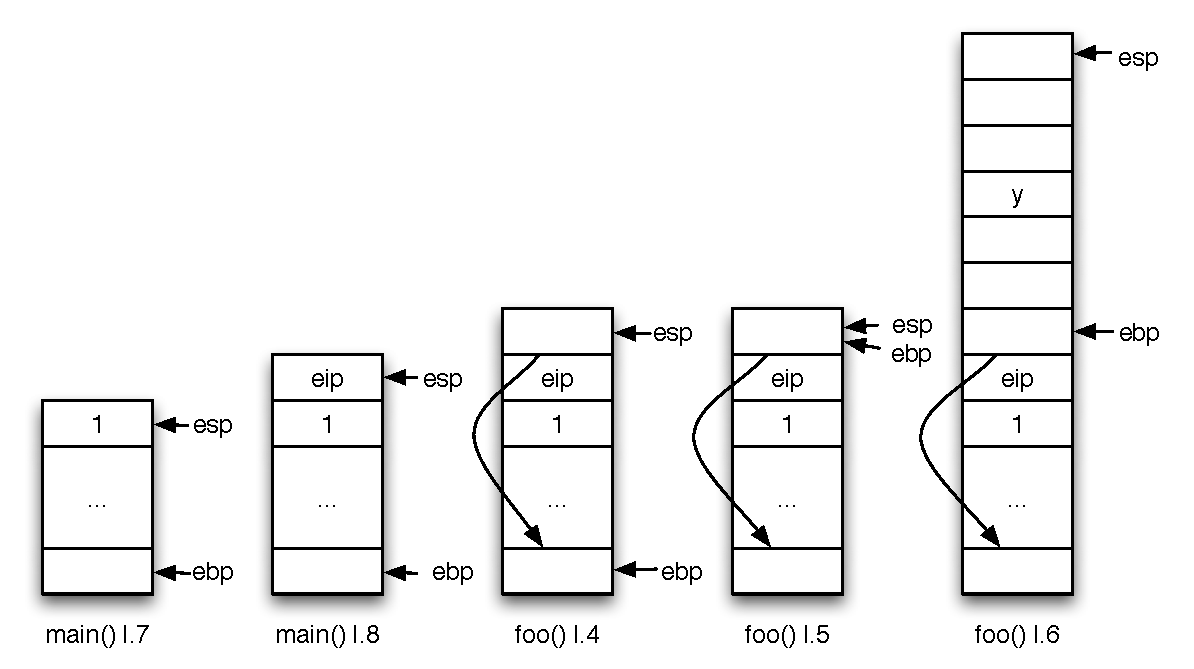
\includegraphics[width=12cm]{figure/function_call.pdf}
 \end{center}
 \caption{関数\icode{foo}呼び出し時の実行時スタック管理}
 \label{185859_11Apr06}
\end{figure}

\icode{foo}を呼び出すとき、\icode{foo}の終了時それぞれについて、上に示し
た機械語命令を追っていこう。まず\icode{foo}の呼び出し時である(図
\ref{185859_11Apr06})。
\begin{enumerate}
 \item \icode{main}の7行目: 実引数の設定。\icode{(\%esp)}、すなわちスタッ
       クポインタの指し示している実行時スタック領域(実行時スタックの先頭)
       に1を格納する。これが$x$に対応する実引数になる\footnote{ここでは示
       していないが、6行目以前では、実行時スタックの先頭には何も値が格納
       されていない。したがって、実行時スタックの先頭の値が上書きされるこ
       とはない。}。
 \item \icode{main}の8行目: \icode{foo}関数の呼び出し。\icode{call}命令で
       は、(命令ポインタ\icode{\%eip}の値$+1$)が実行時スタックにプッシュ
       され(\icode{\%eip}の退避)、\icode{\_foo}ラベル、すなわち関数
       \icode{foo}の3行目の番地が\icode{\%eip}に格納される。したがって、
       次に実行される機械語命令は\icode{foo}の3行目になる。
       \label{181636_11Apr06}
 \item \icode{foo}の3行目: ラベルだけなので、何も行われない。
 \item \icode{foo}の4行目: ベースポインタ\icode{\%ebp}の現在の値、すなわ
       ち\icode{foo}呼び出し前のベースポインタの値を実行時スタックにプッ
       シュする。(\icode{\%ebp}の退避)
       \label{181349_11Apr06}
 \item \icode{foo}の5行目: スタックポインタ\icode{\%esp}の現在の値を
       \icode{\%ebp}に格納する。これにより、\icode{foo}の実行に入る前のス
       タックポインタの値がベースポインタ\icode{\%ebp}に退避されたことに
       なる。(\icode{\%esp}の退避)
       \label{181051_11Apr06}
 \item \icode{foo}の6行目: スタックポインタ\icode{\%esp}の値を24減らす。
       これは、実行時スタックに要素を6個積んだことに相当している。この中
       には、局所変数$y$の領域\footnote{\icode{-12(\%ebp)}、すなわちこの時
       点でのベースポインタから3要素分上の領域である。}なども含まれてい
       る。
 \item \icode{foo}の7-9行目: 局所変数$y$の初期化。実引数$x$の領域は
       \icode{8(\%ebp)}、つまりこの時点でのベースポインタから2要素分下の
       領域であることに注意せよ。
\end{enumerate}

\begin{figure}
 \begin{center}
  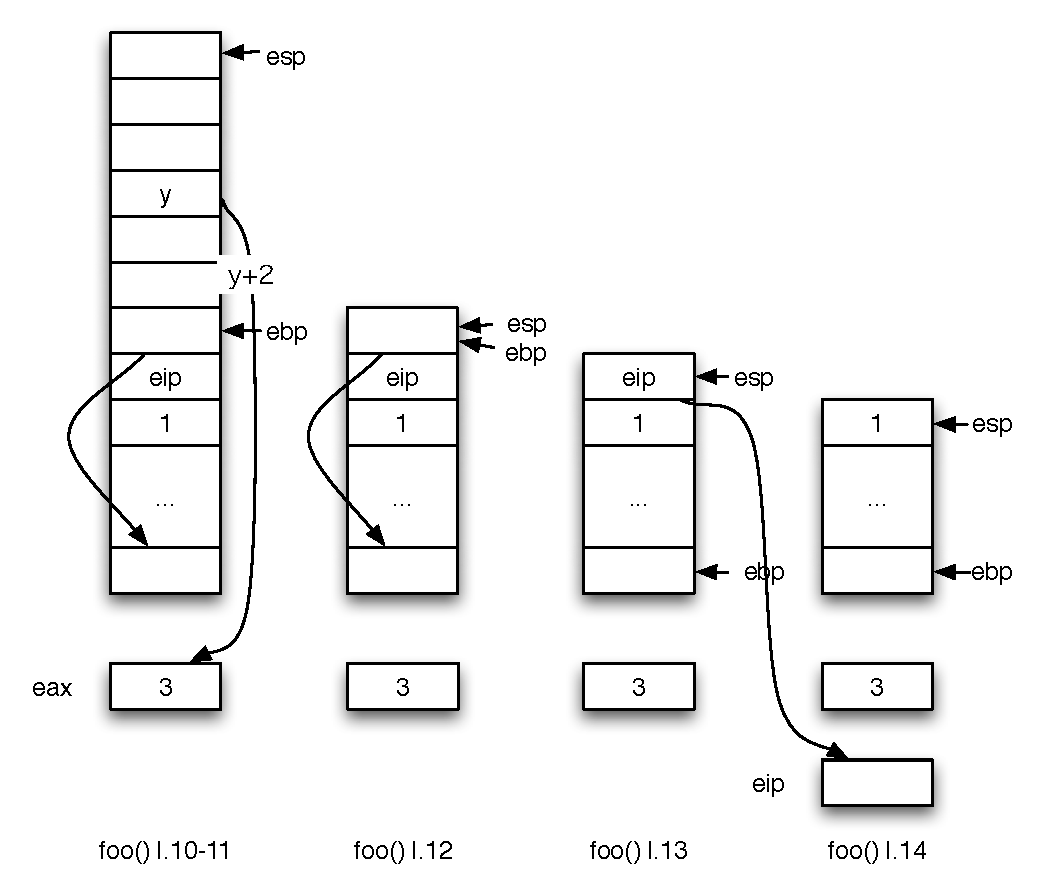
\includegraphics[width=12cm]{figure/function_return.pdf}
 \end{center} 
 \caption{関数\icode{foo}からの戻り処理}
 \label{191124_11Apr06}
\end{figure}

次に関数\icode{foo}の終了時の処理を追ってみる(図\ref{191124_11Apr06})。

\begin{enumerate}
 \item \icode{foo}の10-11行目: 返り値の設定。Pentiumプロセッサでは通常、
       関数からの返り値は汎用レジスタ\icode{\%eax}を使って、呼び出し元に
       受け渡される。ここでも、$y+2$の計算結果が\icode{\%eax}に格納されて
       いる。
 \item \icode{foo}の12行目: 現在のベースポインタ\icode{\%ebp}の値をスタッ
       クポインタ\icode{\%esp}に格納する。呼び出し時の処理
       \ref{181051_11Apr06}で、呼び出し前のスタックポインタの値を
       \icode{\%ebp}に退避していたことに注意せよ。つまり、ここで
       \icode{\%esp}を呼び出し前の状態に復帰している。
 \item \icode{foo}の13行目: 実行時スタックの先頭の要素をポップし、ベース
       ポインタ\icode{\%ebp}に格納している。呼び出し前の処理
       \ref{181349_11Apr06}で、呼び出し前のベースポインタの値を実行時スタッ
       クに退避していたことに注意せよ。つまり、ここで\icode{\%ebp}を呼び
       出し前の状態に復帰している。
 \item \icode{foo}の14行目: \icode{foo}関数からの戻り。\icode{ret}命令で
       は、実行時スタックの先頭の要素をポップし、命令ポインタ
       \icode{\%eip}に格納する。呼び出し前の処理\ref{181636_11Apr06}で、
       呼び出し前の\icode{\%eip}の値を実行時スタックに退避していたことに
       注意せよ。つまり、ここで\icode{\%eip}を呼び出し前の状態に復帰して
       いる。したがって、次の機械語命令は\icode{call}命令の番地$+1$、すな
       わち\icode{call}命令の次の機械語命令になる。
\end{enumerate}

関数呼び出し時、および関数終了時には、常に上記のような処理が行われる。た
だし実際には、他の汎用レジスタの退避・復帰のための機械語命令列も加えられ
ることがある。

%#!platex main

\chapter{$BL\E*%W%m%0%i%`@8@.(B}

$BK\9V5A$N:G8e$H$7$F!"L\E*%W%m%0%i%`$N@8@.$K$D$$$F=R$Y$k!#$?$@$7!"(BC$B8@8l$N9=(B
$BJ8$9$Y$F$r07$&$HFbMF$,J#;($K$J$k$N$G!"$3$3$G$O35N,$r=R$Y$k$K$H$I$a$k!#$^(B
$B$?(B\ref{083441_12Apr06}$B>O$K0z$-B3$-!"6qBN@-$r;}$?$;$k$?$a$K!"(BPentium $B%W%m(B
$B%;%C%5$N(BAT\&T$B7A<0%"%;%s%V%j8@8l$rL\E*8@8l$H$9$k$,!"K\>O$G=R$Y$kFbMF$OHFMQ(B
$BE*$J$b$N$G$"$k!#(B

% $B9=J8<gF3Dj5A$K$h$kCf4V%3!<%I@8@.$N35N,!#%"%;%s%V%j8@8l@8@.$NNc!#(B

$B$^$:=i$a$K!"(BC$B8@8l$NBeI=E*$JJ8$K$D$$$F!"$I$N$h$&$J5!3#8l%3!<%I$r@8@.$9$l$P(B
$B$$$$$N$+=R$Y$k!#<!$K!"$=$N$$$/$D$+$K$D$$$F!"2r@OLZ$+$i%3!<%I$r@8@.$9$kJ}(B
$BK!$K$D$$$F8!F$$9$k!#(B

\section{C$B8@8l$NJ8$KBP$9$k5!3#8l%3!<%I(B}

\subsection{$BJ#J8(B}

C$B8@8l$NJ#J8$O<!$N$h$&$J7A<0$G$"$k!#(B
\begin{quote}
 \icode{\{ $$B@k8@J8(B_1$; $\cdots$ $$B@k8@J8(B_n$; $$BJ8(B_1$; $\cdots$ $$BJ8(B_m$; \}}
\end{quote}
$B!V@k8@J8!W$H$OJQ?t$N@k8@!"!VJ8!W$H$O@k8@J80J30$N(BC$B8@8l$NJ8$G$"$k!#(BC$B8@8l$G(B
$B$O!"J#J8$N@hF,$KJQ?t$N@k8@$rCV$/$3$H$,$G$-!"J#J8Fb$G@k8@$5$l$?JQ?t$O!"$=(B
$B$NJ#J8Fb$G$N$_M-8z$J6I=jJQ?t$H$J$k!#(B

$B$3$l$KBP1~$9$k5!3#8l%3!<%I$O!"<!$N$h$&$J9=B$$K$J$k!#(B
\begin{quote}
 $$B@k8@J8(B_1, \cdots, $B@k8@J8(B_n$$B$KBP1~$9$kJQ?tNN0h$N3NJ](B\\
 $$B@k8@J8(B_1$$B$N=i4|2=!J$b$7$"$l$P!K(B \\
 $\cdots$ \\
 $$B@k8@J8(B_n$$B$N=i4|2=!J$b$7$"$l$P!K(B \\
 $$BJ8(B_1$$B$N<B9T(B \\
 $\cdots$ \\
 $$BJ8(B_m$$B$N<B9T(B \\
 $B6I=jJQ?tNN0h$N2rJ|(B
\end{quote}
$B6I=jJQ?tNN0h$N3NJ]$O!"6qBNE*$K$O!"<B9T;~%9%?%C%/>e$K6I=jJQ?tJ,$NNN0h$r(B
$B!J(B\icode{push}$BL?Na$J$I$G!K@Q$`$3$H$KAjEv$9$k!#$?$@$7!"JQ?t$N=i4|2=$d(B$$BJ8(B_1,
\cdots, $BJ8(B_m$$B$GJQ?t$N;2>H$,5/$3$k$?$a!"$=$l$>$l$N6I=jJQ?t$NNN0h$,$I$3$K3N(B
$BJ]$5$l$?$N$+!"J#J8$N%3!<%I@8@.Cf!"5-21$7$F$*$/I,MW$,$"$k!#$3$l$ODL>o!"3N(B
$BJ]$5$l$?NN0h$NHVCO$r5-9fI=$K=q$-9~$`$3$H$GBP=h$9$k!#Nc$($P!"(B
\begin{quote}
 \icode{int x = 10;}
\end{quote}
$B$H$$$&@k8@J8$KBP$7$F(B\icode{x}$B$NNN0h$r<B9T;~%9%?%C%/>e$K!JNc$($P(B
\icode{-16(\%ebp)}$B$K!K3NJ]$9$k$H$9$k$H!"(B\icode{-16(\%ebp)}$B$r5-9fI=$N(B
\icode{x}$B$N9`L\$K=q$-9~$`!#<!$$$G$3$N=i4|2=$H$7$F!"<!$N$h$&$J5!3#8l$r@8@.(B
$B$9$k!#(B
\begin{quote}
\begin{lstlisting}[language={[x86masm]Assembler}]
 movl  -16(%ebp), 10
\end{lstlisting}
\end{quote}

$BJ#J8$NCf$G3NJ]$7$?6I=jJQ?tNN0h$O!"J#J8=*N;;~$K!J(B\icode{pop}$BL?Na$J$I$G!K<B9T(B
$B;~%9%?%C%/$+$i2<$m$9$h$&$K$9$k!#(B

\subsection{$B>r7oJ8(B}

C$B8@8l$N>r7oJ8$NE57?E*$J7A$O<!$N$h$&$K$J$k!#(B
\begin{quote}
 \icode{if ({\rm $B>r7o<0(B}) $$BJ8(B_1$ else $$BJ8(B_2$}
\end{quote}
$B$3$l$KBP1~$9$k5!3#8l%3!<%I$O<!$N$h$&$K$J$k!#(B
\begin{quote}
 \begin{tabular}{ll}
  & $B>r7o<0$r7W;;$7!"7k2L$r%l%8%9%?(B$R$$B$K3JG<(B \\
  & \icode{cmpl $R$, 0} \\
  & \icode{je $L_1$} \\
  & $$BJ8(B_1$$B$N<B9T(B\\
  & \icode{jmp $L_2$}\\
  $L_1$: & $$BJ8(B_2$$B$N<B9T(B \\
  $L_2$: & \\
 \end{tabular}
\end{quote}
C$B8@8l$G$O!">r7o<0$,(B0$B0J30$J$i??!J(B$$BJ8(B_1$$B$,<B9T!K!"(B0$B$J$i56!J(B$$BJ8(B_2$$B$,<B9T!K$H(B
$B8+$J$5$l$k$3$H$KCm0U$5$l$?$$!#(B

\subsection{$B7+$jJV$7J8(B}

$B$3$3$G$O7+$jJV$7J8$N$&$A(B while $BJ8$N$_$r<h$j>e$2$k!#(Bwhile$BJ8$N7A<0$O<!$N$h(B
$B$&$K$J$k!#(B
\begin{quote}
 \icode{while ({\rm $B>r7o<0(B}) {\rm $BJ8(B}}
\end{quote}
$B$3$l$KBP$9$k5!3#8l%3!<%I$O<!$N$h$&$K$J$k!#(B
\begin{quote}
\begin{tabular}{ll}
 $L_1$: & $B>r7o<0$r7W;;$7!"7k2L$r%l%8%9%?(B$R$$B$K3JG<(B \\
        & \icode{cmpl $R$, 0} \\
        & \icode{je $L_2$} \\
        & \icode{jmp $L_1$} \\
 $L_2$: & \\
\end{tabular}
\end{quote}
$B$b$7(Bwhile$BJ8$NCf$K(B\icode{break}$BJ8$,$"$l$P!"!J(Bwhile$BJ8$+$iC&=P$9$k$H$$$&$3$H(B
$B$G$"$k$+$i!K(B\icode{jmp $L_2$}$B$rA^F~$9$l$P$h$$!#$^$?(B\icode{continue}$BJ8$,$"(B
$B$l$P!J<!$N7+$jJV$7$K?J$`$H$$$&$3$H$G$"$k$+$i!K(B\icode{jmp $L_1$}$B$rA^F~$9$l$P(B
$B$h$$!#(B

\subsection{$B<0J8(B}

$B<0J8$O!"(BC$B8@8l$NBeF~J8$d4X?t8F$S=P$7$NAm>N$G$"$k(B\footnote{$B@53N$K$O!"<0(B$e$
$B$r<B9T$9$k$@$1$NJ8$G$"$k!#(B$e$$B$KJQ?t$X$NBeF~$,4^$^$l$k>l9g$K$O!"I{:nMQ$K$h$C(B
$B$FJQ?t$K7W;;7k2L$NCM$,;D$k$H$_$J$5$l$k!#%W%m%0%i%`<B9T$NI{:nMQ$K$D$$$F$O(B
$B!V7W;;5!8@8l(BI$B!W$N9V5AFbMF$r;2>H$N$3$H!#(B}$B!#4X?t8F$S=P$7$,$I$N$h$&$J%3!<%I(B
$B$K$J$k$+$O(B\ref{181902_17Apr06}$B@a$G=R$Y$?$N$G!"$3$3$G$OBeF~J8$K$D$$$F<h$j(B
$B>e$2$k!#(B

$BJQ?t(B\icode{v}$B$X$NBeF~J8(B\icode{v = $e'$;}$B$KBP$9$k5!3#8l%3!<%I$O<!$N$h$&$K(B
$B$J$k!#$?$@$7(B$loc(v)$$B$O!"JQ?t(B\icode{v}$B$,3d$jEv$F$i$l$F$$$kHVCO$rI=$9!#(B
\begin{quote}
 $e'$$B$N7W;;$r9T$$!"7k2L$r%l%8%9%?(B$R$$B$K3JG<(B \\
 \icode{movl $R$, $loc(v)$}
\end{quote}

$B$7$?$,$C$F!"(B\icode{i = foo();}$B$N$h$&$K(B$e'$$B$,4X?t8F$S=P$7$N>l9g$K$O!"<!$N(B
$B$h$&$J%3!<%I$,@8@.$5$l$k!#4X?t$+$i$NJV$jCM$O%l%8%9%?(B\icode{\%eax}$B$K3JG<$5(B
$B$l$k$3$H$r;W$$=P$7$F$*$/$3$H!#(B
\begin{quote}
 \icode{call \_foo} \\
 \icode{movl \%eax, $loc(i)$}
\end{quote}

$e'$$B$,;;=Q<0$N>l9g!"4pK\E*$J%3!<%I@8@.$N<j=g$O<!$N$h$&$K$J$k!#Fs9`;;=Q1i(B
$B;;;R(B$\circ$$B$KBP1~$7$F!"5!3#8l$N;;=QL?Na(B$inst$$B$,MQ0U$5$l$F$$$k$J$i$P!";;(B
$B=Q<0(B$e_1 \circ e_2$$B$N$?$a$N5!3#8l%3!<%I$O<!$N$h$&$K$J$k!#(B
\begin{quote}
 $e_1$$B$NCM$r%l%8%9%?(B$R$$B$K%m!<%I(B \\
 \icode{$inst$ $e_2$$B$NCM(B, $R$}
\end{quote}
$BNc$($P<0(B$x+y$$B$KBP$7$F$O<!$N$h$&$J%3!<%I$,@8@.$5$l$k!#(B
\begin{quote}
 \icode{movl $loc(x)$, $R$} \\
 \icode{addl $loc(y)$, $R$}
\end{quote}
$B$^$?<0(B$a*b+y$$B$KBP$7$F$O<!$N$h$&$J%3!<%I$,@8@.$5$l$k!#(B
\begin{quote}
 \icode{movl $loc(a)$, $R$} \\
 \icode{imul $loc(b)$, $R$} \\
 \icode{movl $R$, $R'$} \\
 \icode{addl $loc(y)$, $R'$}
\end{quote}
$a*b$$B$N7W;;7k2L$O%l%8%9%?(B$R$$B$K;D$C$F$$$k$N$G!"(B3$B9TL\$G$O%l%8%9%?(B$R$$B$NCM$r(B
$B%l%8%9%?(B$R'$$B$K%m!<%I$9$k!"$H$$$&%3!<%I$r@8@.$7$F$$$k!#(B

\subsection{$B%3!<%I@8@.$NLdBj(B}

$B$3$3$^$G$N@a$G=R$Y$F$-$?5!3#8l%3!<%I$O86B'E*$J$b$N$G!"<B:]$O$5$i$K9)IW$r(B
$B9T$&I,MW$,$"$k!#FC$K!"%l%8%9%?$N3d$jEv$F$HL5BL$J%3!<%I$N=|5n$O=<J,Cm0U$7(B
$B$J$1$l$P$J$i$J$$!#(B

$BNc$H$7$F!">e$G5s$2$?<0(B$a*b+y$$B$KBP$9$k<!$N%3!<%I$r9M$($k!#(B
\begin{quote}
 \icode{movl $loc(a)$, $R$} \\
 \icode{imul $loc(b)$, $R$} \\
 \icode{movl $R$, $R'$} \\
 \icode{addl $loc(y)$, $R'$}
\end{quote}
$B$3$N%3!<%I$G$O!"(B$a*b$$B$N7W;;7k2L$r%l%8%9%?(B$R$$B$K!":G=*7k2L$r%l%8%9%?(B$R'$$B$K(B
$B$=$l$>$l3d$jEv$F$F$$$k!#$7$+$7!"$3$NNc$G$O:G=*7k2L$b(B$R$$B$K3d$jEv$F$F$b9=$o(B
$B$J$$$O$:$G$"$k!#$9$k$H<!$N$h$&$J%3!<%I$K$J$j!"(B3$B$D$N5!3#8lL?Na$G:Q$_!"$^$?(B
$B;HMQ$9$k%l%8%9%?$b(B1$B$D$G:Q$`!#(B
\begin{quote}
 \icode{movl $loc(a)$, $R$} \\
 \icode{imul $loc(b)$, $R$} \\
 \icode{addl $loc(y)$, $R$}
\end{quote}

$BHFMQ%l%8%9%?$N8D?t$O>/$J$$$N$G!"L5BL$J$/HFMQ%l%8%9%?$r;H$$2s$9$3$H$O!"B.(B
$B$$%3!<%I$r@8$_=P$9$N$KBgJQ=EMW$G$"$k!#(B

$B$^$?5!3#8lL?Na$N?t$r8:$i$9$3$H$b=EMW$G$"$k!#!V$?$+$,5!3#8lL?Na(B1$B$D8:$i$7$?(B
$B$H$3$m$G!"Bg$7$FB.$/$J$k$o$1$G$O$J$$!W$H;W$&$+$b$7$l$J$$$,!"$3$l$,(B100$BK|2s(B
$B$N%k!<%W$NCf$N%3!<%I$@$C$?$i$I$&$@$m$&!#(B40$BIC$+$+$C$?7W;;$,(B30$BIC$G:Q$`$+$b(B
$B$7$l$J$$!#(B

$B$$$C$?$s@8@.$7$?%3!<%I$rJQ7A$7!"$h$jB.$/8zN($h$$%3!<%I$K2~NI$9$k$3$H$r(B
{\bfseries $B:GE,2=(B}$B!J(Boptimization$B!K$H$$$&!#K\9V5A$G$O$3$l0J>e?<F~$j$7$J$$(B
$B$,!":GE,2=$r9T$&$K$O!"2r@OLZ$+$i$$$-$J$jL\E*%W%m%0%i%`$N5!3#8lL?Na$r@8@.(B
$B$9$k$N$G$O$J$/!"<!@a$G=R$Y$k$h$&$K!"Cf4VE*$J7A<0$N%3!<%I!JCf4V%3!<%I!K$r(B
$B@8@.$9$k$[$&$,$h$$!#:GE,2=$N$?$a$N%3!<%I2r@O$,!"5!3#8lL?Na$KBP$7$F$h$j$b(B
$BCf4V%3!<%I$KBP$9$k$[$&$,9T$$$d$9$$$+$i$G$"$k!#(B

\section{$BK]Lu%9%-!<%`$K4p$E$/%3!<%I@8@.(B}

$B$3$N@a$G$O!"K]Lu%9%-!<%`$K4p$E$$$F2r@OLZ$+$iCf4V%3!<%I$r@8@.$9$kJ}K!$K$D(B
$B$$$F=R$Y$k!#$?$@$7!"4JC1$N$?$a!"<h$j>e$2$k$N$O;;=Q<0$H(Bwhile$BJ8$K$H$I$a$k!#(B

\subsection{$B;0HVCO%3!<%I(B}

$B$3$3$G$OCf4V%3!<%I$H$7$F(B{\bfseries $B;0HVCO%3!<%I(B}$B!J(Bthree-address code$B!K$H(B
$B$$$&$b$N$rMQ$$$k!#;0HVCO%3!<%I$NJ8$N$&$A!"K\@a$N@bL@$KI,MW$J$b$N$r0J2<$K(B
$B<($9!#$J$*!";0HVCO%3!<%I$NA4L?Na$O(B\cite{aho86:_compiler}$B$N(B8.1$B@a$K$"$k!#(B

\begin{enumerate}
 \item $BBeF~J8(B\icode{x = y $\op$ z}$B!#$3$3$G(B$\op$$B$OFs9`;;=Q1i;;;R$G$"$k!#(B
 \item $BBeF~J8(B\icode{x = $\op$ y}$B!#$3$3$G(B$\op$$B$OC19`1i;;;R!JId9f$NH?E>$rI=$9(B
       $-$$B$J$I!K$G$"$k!#(B
 \item $BBeF~J8(B\icode{x = y}$B!#(B$y$$B$NCM$r(B$x$$B$KBeF~$9$k!#(B
 \item $BL5>r7oJ,4t(B\icode{goto $L$}$B!#(B$L$$B$r%i%Y%k$K;}$DJ8$KJ,4t$9$k!#(B
 \item $B>r7oIU$-J,4t(B\icode{if x $\op$ y goto $L$}$B!#(B$\op$$B$OHf3S1i;;;R$G$"$k!#(B
       \icode{x $\op$ y}$B$,@.N)$9$l$P(B$L$$B$r%i%Y%k$K;}$DJ8$KJ,4t$9$k!#@.N)$7(B
       $B$J$1$l$P<!$NJ8$K@)8f$r0\$9!#(B
\end{enumerate}

$B$3$l$i$+$iJ,$+$k$h$&$K!";0HVCO%3!<%I$G$O!"J8$N1&JU$K$O1i;;;R$r$?$+$@$+(B1
$B$D$7$+5v$5$J$$!#(B2$B$D0J>e1i;;;R$r4^$`;;=Q<0$K$D$$$F$O!"0l;~JQ?t$rMQ$$$F!"J#(B
$B?t$NJ8$NNs$KK]Lu$7$J$1$l$P$J$i$J$$!#$?$H$($P(B$x + y * z$$B$H$$$&86;O8@8l$N<0(B
$B$O!"<!$N$h$&$JJ8$NNs$K$J$k!#(B
\begin{quote}
 \icode{t1 = y * z} \\
 \icode{t2 = x + t1}
\end{quote}

\subsection{$B;0HVCO%3!<%I$r@8@.$9$kK]Lu%9%-!<%`(B}

$BB?$/$N>l9g!";0HVCO%3!<%I$O(B\ref{195223_17Apr06}$B@a$G=R$Y$?(BS$BB0@-Dj5A$d(BL$BB0@-(B
$BDj5A$rMQ$$$F!"2r@OLZ$+$i@8@.$9$k$3$H$,$G$-$k!#(B

$B$^$:!"1&JU$K;;=Q<0$r;}$DBeF~J8$r9M$($h$&!#@8@.5,B'$O<!$N$h$&$K$J$k!#(B
\begin{align*}
 S & \rightarrow \icode{id} = E \\
 E & \rightarrow E + E \\
 E & \rightarrow E \ast E \\
 E & \rightarrow - E \\
 E & \rightarrow ( E ) \\
 E & \rightarrow \icode{id}
\end{align*}
\begin{figure}
 \begin{center}
  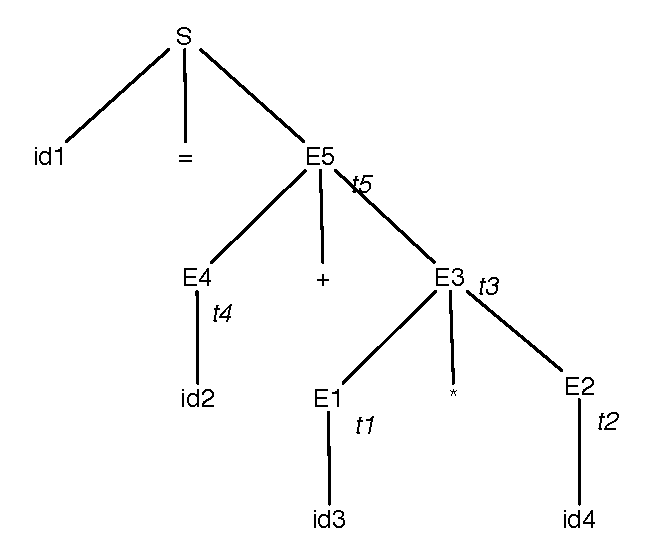
\includegraphics{figure/parse_tree_substitution.pdf}
 \end{center}
 \caption{$BBeF~J8(B\icode{id = id + id * id}$B$KBP$9$k2r@OLZ(B}
 \label{142215_18Apr06}
\end{figure}
$B$3$NJ8K!$K4p$E$-!"BeF~J8(B\icode{id = id + id * id}$B$N2r@OLZ$r:n$k$H?^(B
\ref{142215_18Apr06}$B$N$h$&$K$J$k!#(B

$B$3$NBeF~J8$KBP$9$k;0HVCO%3!<%I$K$O!"$5$^$6$^$J2DG=@-$,$"$k!#$3$3$G$O!"2r(B
$B@OLZCf$NFbIt@aE@!JHs=*C<5-9f!K(B$E$$B$=$l$>$l$K0l;~JQ?t$r3d$j?6$k$b$N$H$7$h$&(B
$B!J?^(B\ref{142215_18Apr06}$BCf$N<P;zBN!K!#$9$k$H!"BP1~$9$k;0HVCO%3!<%I$O<!$N(B
$B$h$&$K$J$k(B\footnote{$BL@$i$+$K>iD9$JJ8$,4^$^$l$F$$$k$,!"$3$l$O:GE,2=$K$h$C(B
$B$F2~A1$9$k$b$N$H$7!"$3$3$G$OLdBj$K$7$J$$!#(B}$B!#%3!<%ICf!"4X?t(B$val(id)$$B$O<1(B
$BJL;R(B$id$$B$NCM$rI=$9!#(B
\begin{align*}
 t_4 & = val(id_2) && E_4 \\
 t_1 & = val(id_3) && E_1 \\
 t_2 & = val(id_4) && E_2 \\
 t_3 & = t_1 \ast t_2 && E_3 \\
 t_5 & = t_4 + t_3 && E_5 \\
 id_1 & = t_5 && S
\end{align*}

$BL@$i$+$K3FJ8$O$=$l$>$l1&$K<($7$?FbIt@aE@$KBP1~$7$F$*$j!"$+$D$=$N@aE@$N;R(B
$B@aE@$N0l;~JQ?t$N$_$K0MB8$7$F$$$k!#$7$+$b!"BP1~$9$kFbIt@aE@$N=P8==g$O!"2r(B
$B@OLZ$r5"$j$,$1=g$K$?$I$C$?=g$K0lCW$7$F$$$k!#(B

$B$7$?$,$C$F!">e5-$N;0HVCO%3!<%I$O(BS$BB0@-Dj5A$K$h$C$F@8@.$9$k$3$H$,2DG=$G$"$k!#(B
$B0J2<$K;0HVCO%3!<%I$r@8@.$9$k(BS$BB0@-Dj5A$r<($9!#$3$3$G!"Hs=*C<5-9f$NB0@-(B
$place$$B$O!"$=$NHs=*C<5-9f$KBP1~$9$k0l;~JQ?tL>$rJ];}$7$F$$$k!#$^$?4X?t(B
$newtemp()$$B$O?7$?$J0l;~JQ?t$r@8@.$9$k4X?t!"(B$gencode()$$B$O0z?t$+$i;0HVCO%3!<(B
$B%I$r@8@.$9$k4X?t$G$"$k!#(B
\begin{align*}
 S \rightarrow & \icode{id} = E\ \{ gencode(\icode{id = } E.place);\} \\
 E \rightarrow & \{E.place = newtemp(); \} \\
   & E_1 + E_2\ \{ gencode(E.place = E_1.place + E_2.place); \}\\
 E \rightarrow & \{E.place = newtemp(); \} \\
   & E_1 \ast E_2\ \{ gencode(E.place = E_1.place * E_2.place); \} \\
 E \rightarrow & \{E.place = newtemp(); \} \\
   & - E_1\ \{ gencode(E.place = - E_1.place); \}\\
 E \rightarrow & \{E.place = newtemp(); \} \\
   & ( E_1 )\ \{ gencode(E.place = E_1.place); \} \\
 E \rightarrow & \{E.place = newtemp(); \} \\
   & \icode{id}\ \{ gencode(E.place = val(\icode{id})); \}
\end{align*}

$B$b$&0l$D!"K]Lu%9%-!<%`$rMQ$$$?;0HVCO%3!<%I@8@.$NNc$H$7$F!"(Bwhile$BJ8$r<h$j>e(B
$B$2$k!#(Bwhile$BJ8$N@8@.5,B'$O<!$N$h$&$K$J$k!#(B
\begin{align*}
 S & \rightarrow \icode{while}\ (E)\ S
\end{align*}
$B$3$l$KBP1~$9$k;0HVCO%3!<%I$O<!$N$h$&$K$J$k!#E:;z$N(B$r$$B$O1&JU$K=P8=$9$k5-9f(B
$B$G$"$k$3$H$rI=$9!#(B
\begin{quote}
 \begin{tabular}{ll}
  $L_1$: & $E$$B$KBP$9$k%3!<%I(B \\
        & \icode{if $E.place$ = 0 goto $L_2$} \\
        & $S_r$$B$KBP$9$k%3!<%I(B \\
        & \icode{goto $L_1$} \\
  $L_2$: & \\
 \end{tabular}
\end{quote}

$B$3$l$bBeF~J8$HF1MM!"(BS$BB0@-Dj5A$rMQ$$$F2r@OLZ$+$i@8@.$9$k$3$H$,2DG=$G$"$k!#(B
$B0J2<$K$3$N;0HVCO%3!<%I$r@8@.$9$k(BS$BB0@-Dj5A$r<($9!#$3$3$GB0@-(B$begin, end$
$B$O$=$l$>$l(B$L_1, L_2$$B$KAjEv$9$k%i%Y%k$rJ];}$9$k!#$^$?4X?t(B$newlabel()$$B$O!"(B
$B?7$?$J%i%Y%k$r@8@.$9$k4X?t$G$"$k!#(B
\begin{align*}
 S \rightarrow & \{ S.begin = newlabel();\ S.end = newlabel(); \} \\
               & \{ gencode(S.begin\colon); \} \\
               & \icode{while}\ (E)\ \{ /*$B$3$3$^$G$G(BE$B$N%3!<%I$,@8@.$5$l(B
 $B$F$$$k(B */\} \\
               & \{ gencode(\icode{if}\ E.place = 0\ \icode{goto}\ S.end);
 \} \\
               & S\ \{ /*$B$3$3$^$G$G(BS_r$B$N%3!<%I$,@8@.$5$l$F$$$k(B */\} \\
               & \{ gencode(\icode{goto}\ S.begin); \} \\
               & \{ gencode(S.end\colon); \} 
\end{align*}

%%#!platex main

\chapter{練習問題}

\section{正則表現・有限オートマトン}

\begin{exercise}
 次の言語を表す正則表現を示せ。
 \begin{enumerate}
  \item アルファベット$\{0, 1\}$上の記号列のうち、0から始まり1が0回以上続
	くもの全体からなる言語
  \item アルファベット$\{a, b, c\}$上の記号列のうち、1個以上の$a$と1個以
	上の$b$を含むもの全体からなる言語
  \item アルファベット$\{0, 1\}$上の記号列のうち、0と1が交互に出現するも
	の全体からなる言語
 \end{enumerate}
\end{exercise}
\begin{exercise}
 正則表現 $(0 \mid 1)^\ast 0(0\mid 1)(0\mid 1)$ が表す言語は何か。言葉で説明せよ。
\end{exercise}
\begin{exercise}
 C言語の空白記号は、空白($_{\sqcup}$)、タブ(\verb|\t|)、改行
 (\verb|\n|)が1個以上並んだ文字列である。これを正則表現で表せ。
\end{exercise}
\begin{exercise}
 C言語の16進定数は 0x あるいは 0X で始まり、数字および a, b, c, d, e, f,
 A, B, C, D, E, F が1個以上続く。これを正則表現で表せ。
\end{exercise}
\begin{exercise}
 C言語の識別子はA〜Z, a〜z, 0〜9, 下線(\underline{ })からなる文字列であ
 る。ただし、最初の文字に数字を使うことはできない。これを正則表現で表せ。
\end{exercise}
\begin{exercise}
 アルファベットを$\{0, 1\}$とするとき、次の言語を受理する有限オートマト
 ンを示せ。
 \begin{enumerate}
  \item $00$で終わる記号列全体
  \item $011$を途中に含む記号列全体
 \end{enumerate}
\end{exercise}
\begin{exercise}
 正則表現$00(0 \mid 1)^\ast$に対応する有限オートマトンを構成せよ。
\end{exercise}


\section{文脈自由文法}

\begin{exercise}
 次の文脈自由文法について、トークン列 8 - 2 + 6 の解析木を示せ。可能なす
 べての場合を示し、自然な式の意味になるものはどれか示せ。
 \[
  string \rightarrow string + string \mid string - string \mid 0 \mid 1
 \mid 2 \mid 3 \mid 4 \mid 5 \mid 6 \mid 7 \mid 8 \mid 9
 \]
\end{exercise}
\begin{exercise}
 文脈自由文法$S \rightarrow 0 S 1 \mid 0 1$はどのような言語を表すか述べよ。
\end{exercise}
\begin{exercise}
 次の文法を考える。
  \begin{eqnarray*}
   S & \rightarrow & A1B \\
   A & \rightarrow & 0A \mid \epsilon \\
   B & \rightarrow & 0B \mid 1B \mid \epsilon
  \end{eqnarray*}
 この文法に対し、文字列$00101$の最左導出、最右導出を示せ。
\end{exercise}
\begin{exercise}
 文法
 \begin{equation*}
  S \rightarrow aS \mid aSbS \mid \epsilon
 \end{equation*}
 は曖昧である。文字列$aab$に対して、解析木、最左導出、最右導出がそれぞれ
 2つずつ存在することを示せ。
\end{exercise}
\begin{exercise}
 算術式に対する文法
  \begin{eqnarray*}
   E & \rightarrow & E + T \mid T \\
   T & \rightarrow & T * F \mid F \\
   F & \rightarrow & (E) \mid {\bf id}
  \end{eqnarray*}
 を、左再帰でないように変形せよ。
\end{exercise}

\section{構文解析}

\begin{exercise}
 次の文法について以下の問いに答えよ。
 \begin{align*}
  S & \rightarrow AaAb \mid BbBa \\
  A & \rightarrow \epsilon \\
  B & \rightarrow \epsilon
 \end{align*}
 \begin{enumerate}
  \item すべての非終端記号について$\First$と$\Follow$を計算せよ。
  \item この文法はLL(1)文法か。
 \end{enumerate}
\end{exercise}
\begin{exercise}
 次の文法がLL(1)文法かどうか判定せよ。
 \begin{align*}
  S & \rightarrow aA \mid B \mid cC \mid \epsilon \\
  A & \rightarrow aB \mid Ca \\
  B & \rightarrow bC \mid d \\
  C & \rightarrow cA \mid Bc
 \end{align*}
\end{exercise}
\begin{exercise}
 次の文法がLL(1)文法かどうか判定せよ。
 \begin{align*}
  S & \rightarrow aA \mid aAb \\
  A & \rightarrow \epsilon \mid baA
 \end{align*}
\end{exercise}

\section{意味解析}

\begin{exercise}
 次の問いに答えよ。
 \begin{enumerate}
  \item 中置記法の式$9*(6+2)-4$を後置記法に変換せよ。
  \item 得られた後置記法の式をスタック1本を用いて計算することを考える。
	計算の過程を順を追って示せ。
 \end{enumerate}
\end{exercise}
\begin{exercise}
 次に示すのは、0以上の2進整数を表す文脈自由文法を基にした翻訳スキームである。
  \begin{align*}
   S & \rightarrow S' B && \{ S.val = S'.val * 2 + B.val; \}\\
   S & \rightarrow B && \{ S.val = B.val; \}\\
   B & \rightarrow 0 && \{ B.val = 0; \}\\
   B & \rightarrow 1 && \{ B.val = 1; \}
  \end{align*}
 \begin{enumerate}
  \item $11001$に対する(意味動作を含んだ)解析木を示せ。
	\label{152748_11Jul06}
  \item \ref{152748_11Jul06}で示した解析木の根の属性 $val$ を計算せよ。
  \item この翻訳スキームは何を計算するものか、説明せよ。
 \end{enumerate}
\end{exercise}

\section{実行時環境}

\begin{exercise}
 C言語変数の記憶域割付け手法を3つ示し、それぞれどのようなものか説明
 せよ。
\end{exercise}


\bibliographystyle{jplain}
\bibliography{main}

%#!platex main

\chapter*{$BN}=,LdBj$N2rEz(B}

\section*{\ref{134138_29Mar06}$B>O(B}

\paragraph{\ref{ex:intro01}}

$BN,(B

\paragraph{\ref{ex:intro02}}

\verb|x, =, 0, ;, while, (, i, <, 100, ), {, x, +=, i, ;, i, ++, ;, }|

\section*{\ref{151253_30Mar06}$B>O(B}

\paragraph{\ref{ex:cfg_03}}

\begin{center}
 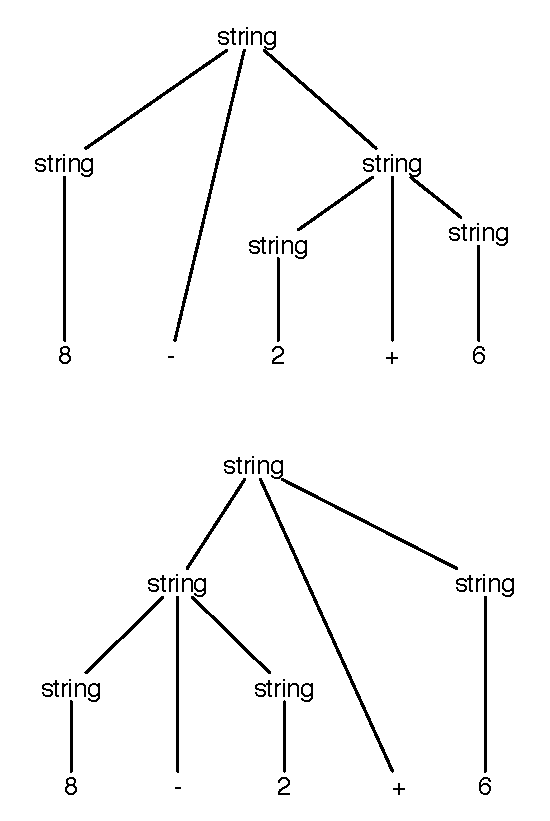
\includegraphics[scale=0.8]{figure/ans_cfg_03.pdf}
\end{center}

$+, -$$B$O:87k9g$N1i;;;R$G$"$j!"3g8L$,$J$1$l$P<0$N:8$+$i7W;;$7$F$$$/(B
$B$N$,@5$7$$0UL#$K$J$k!#$7$?$,$C$F!"2<B&$N2r@OLZ$N$[$&$,<+A3$G$"$k!#(B
$B$3$N$h$&$K!"J8K!$K$h$C$F$O!"F1$85-9fNs$KBP$7$F2r@OLZ$,(B2$BDL$j0J>e9M(B
$B$($i$l$k>l9g$,$"$k!#$3$N$h$&$JJ8K!$r(B{\bfseries $B[#Kf$G$"$k(B}$B$H$$$&!#(B

\paragraph{\ref{ex:cfg_04}}

$0$$B$,(B$n$$B8D(B($n \geq 1$)$BJB$s$@8e$K(B$1$$B$,(B$n$$B8DJB$s$@$h$&$JJ8;zNs$9$Y$F(B
$B$+$i$J$k8@8l!#(B$0, 1$$B$r$=$l$>$l(B$\{, \}$$B$KCV$-49$($F$_$k$H!"$3$l$OBP(B
$B1~4X78$N$H$l$?3g8L$NF~$l;R$rI=$9!#$3$N8@8l$O@5B'8@8l$G$O$J$$Nc$H$7(B
$B$FM-L>$G$"$k!#$D$^$j!"$3$N8@8l$O@5B'I=8=$G$O=q$1$:!"$^$?$3$N8@8l$r(B
$B<uM}$9$kM-8B%*!<%H%^%H%s$b:n$l$J$$!#(B

\paragraph{\ref{ex:cfg_01}}

\[
 S \Rightarrow A1B \Rightarrow 0A1B \Rightarrow 00A1B \Rightarrow
 001B \Rightarrow 0010B \Rightarrow 00101B \Rightarrow 00101
\]
\[
 S \Rightarrow A1B \Rightarrow A10B \Rightarrow A101B \Rightarrow
 A101 \Rightarrow 0A101 \Rightarrow 00A101 \Rightarrow 00101
\]

\paragraph{\ref{ex:cfg_02}}

\begin{eqnarray*}
 E & \rightarrow & TE' \\
 E' & \rightarrow & + TE' \mid \epsilon \\
 T & \rightarrow & FT' \\
 T' & \rightarrow & * FT' \mid \epsilon \\
 F & \rightarrow & (E) \mid \mathbf{id}
\end{eqnarray*}


\end{document}
